\documentclass[12pt]{article}
\usepackage{graphicx,psfrag,epsf}
\usepackage{enumerate}
\usepackage{natbib}
\usepackage{amsfonts}
\usepackage{amsmath}
\usepackage{algorithm}
\usepackage{algorithmic}
\usepackage{amssymb,mathabx}
\usepackage{float}
%\usepackage{cite}
\newcommand{\blind}{0}

\addtolength{\oddsidemargin}{-.75in}%
\addtolength{\evensidemargin}{-.75in}%
\addtolength{\textwidth}{1.5in}%
\addtolength{\textheight}{1.3in}%
\addtolength{\topmargin}{-.8in}%


\begin{document}


%\bibliographystyle{plain}

\def\spacingset#1{\renewcommand{\baselinestretch}%
{#1}\small\normalsize} \spacingset{1}


%%%%%%%%%%%%%%%%%%%%%%%%%%%%%%%%%%%%%%%%%%%%%%%%%%%%%%%%%%%%%%%%%%%%%%%%%%%%%%

\if0\blind
{
  \title{\bf Efficient MCMC Sampling Finite-State Markov Jump Processes and Bayesian Inference}
  \author{  
   %  Vinayak Rao\thanks{
    %The authors gratefully acknowledge}\hspace{.2cm}\\
    %Department of Statistics, Purdue University\\
    %and \\
    Boqian Zhang \\
    Department of Statistics, Purdue University\\
    Vinayak Rao\\
    Department of Statistics, Purdue University\\
    }
  \maketitle
} \fi

\if1\blind
{
  \bigskip
  \bigskip
  \bigskip
  \begin{center}
    {\LARGE\bf Title}
\end{center}
  \medskip
} \fi

\bigskip
\begin{abstract}
Abstrct.
\end{abstract}
\noindent%
{\it Keywords:}  Markov jump process, MCMC, Metropolis Hasting sampler, Bayesian inference

\spacingset{1.45}
\section{Introduction}
\label{sec:intro}
In this paper, we tackled the problem of sampling MJP parameters from the posteriors, efficiently, using Metropolis Hasting algorithm.
\section{Metropolis Hasting for Bayesian Inference using FFBS  within the Gibbs Sampling On MJPs}~
\setlength{\unitlength}{0.8cm}
  \begin{figure}[H]
  \centering
  \begin{minipage}[!hp]{0.45\linewidth}
  \centering
    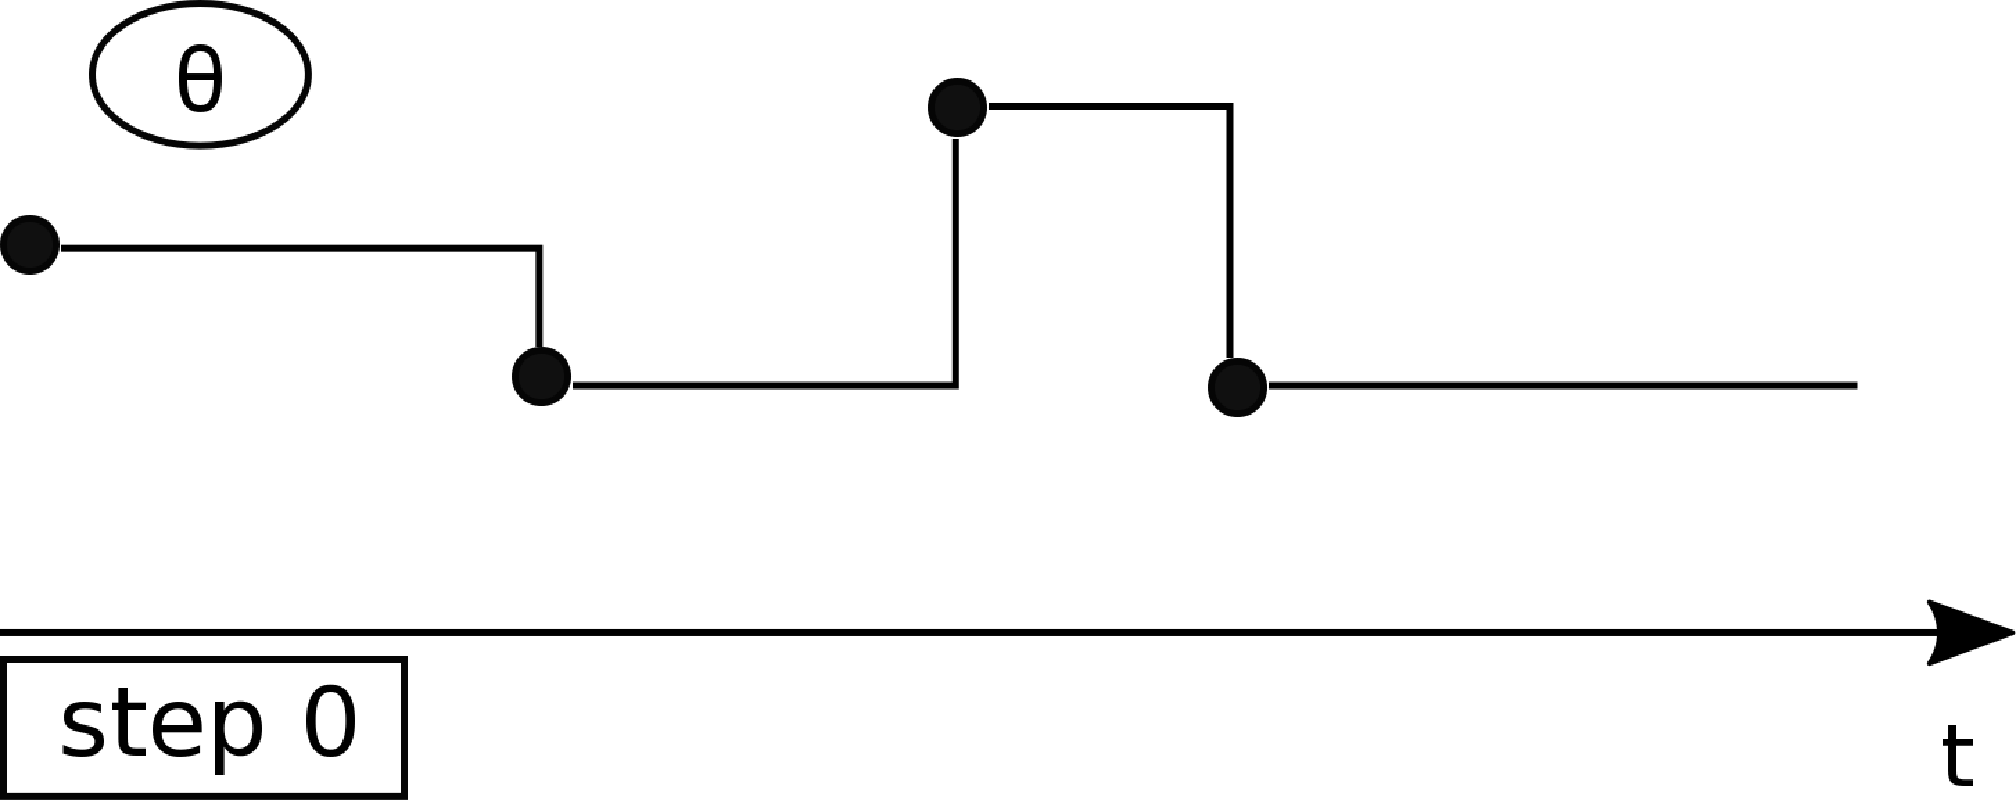
\includegraphics [width=0.70\textwidth, angle=0]{figs/plotn0.png}
      \end{minipage}
  \begin{minipage}[!hp]{0.45\linewidth}
  \centering
    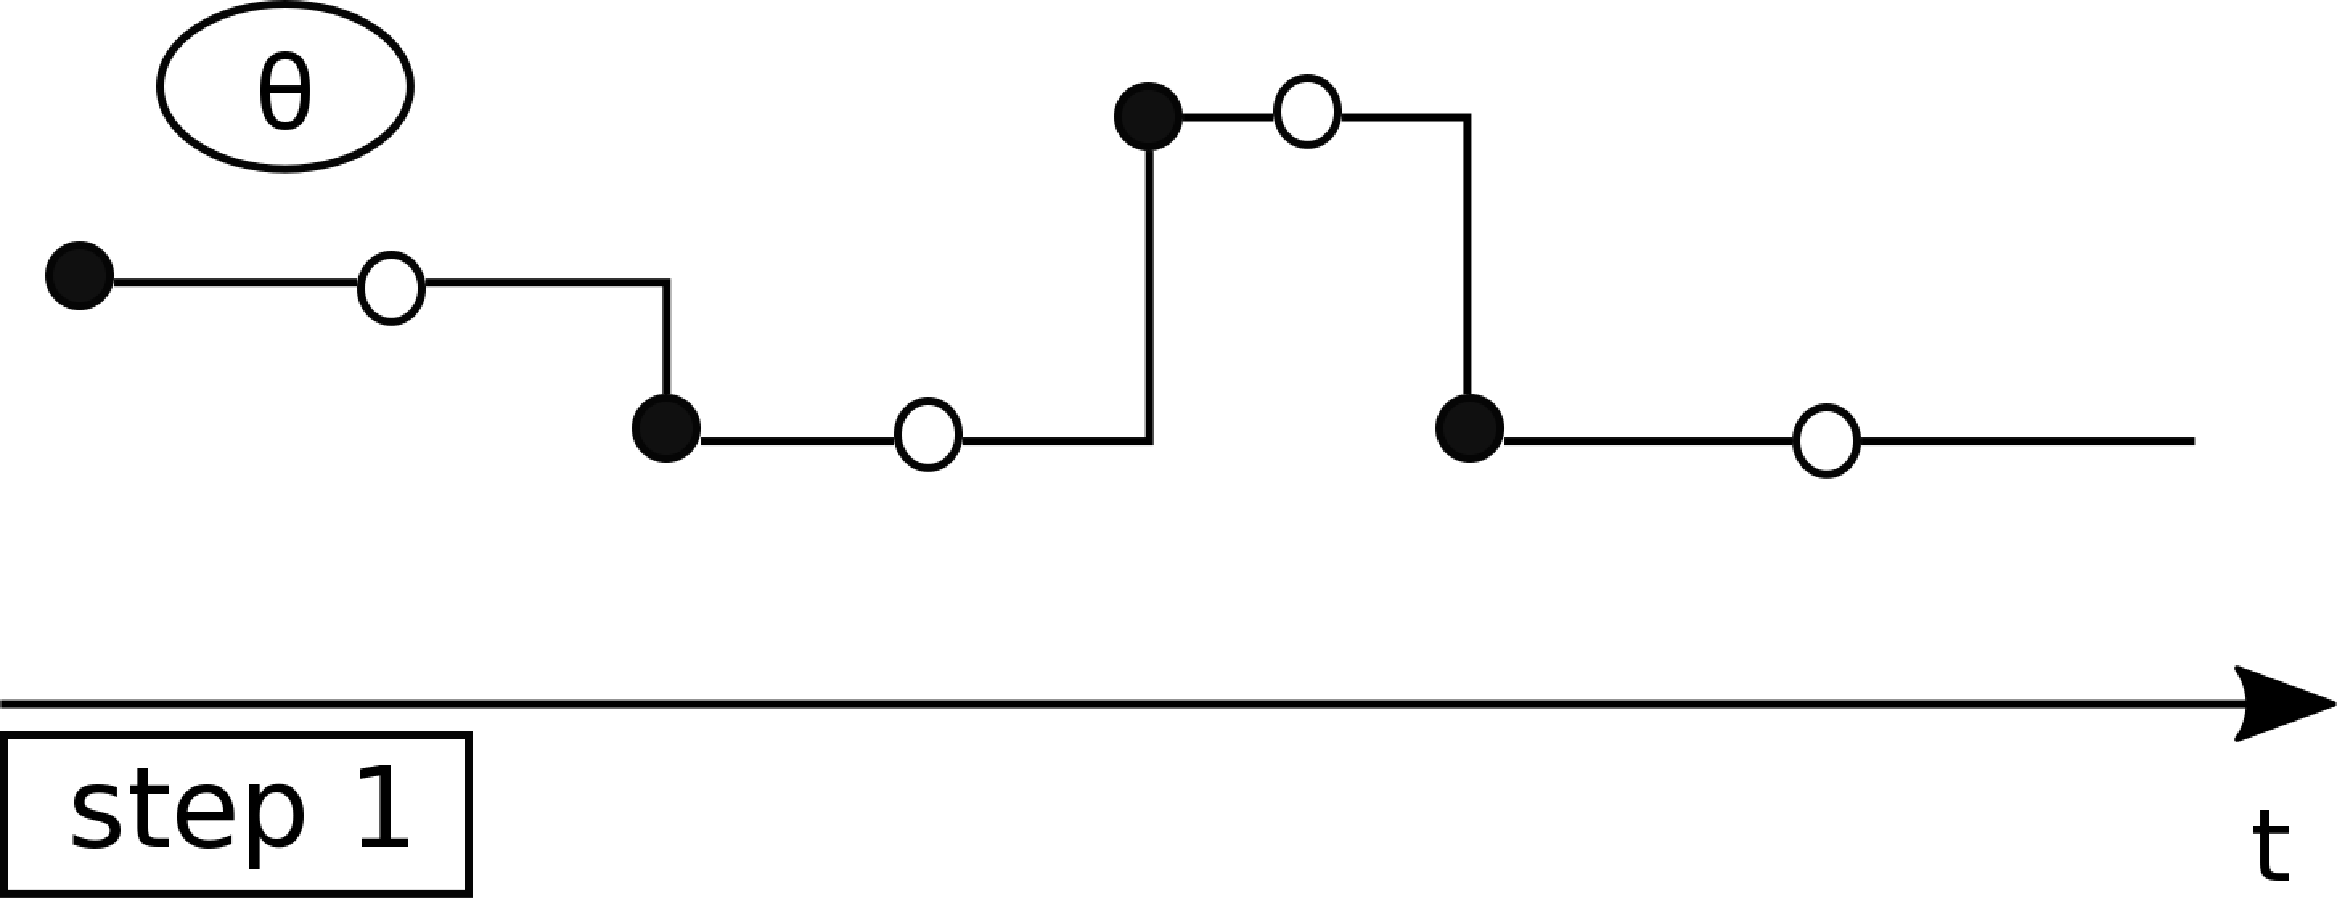
\includegraphics [width=0.70\textwidth, angle=0]{figs/plotn1.png}
    \vspace{-0 in}
  \end{minipage}
  \begin{minipage}[!hp]{0.45\linewidth}
  \centering
    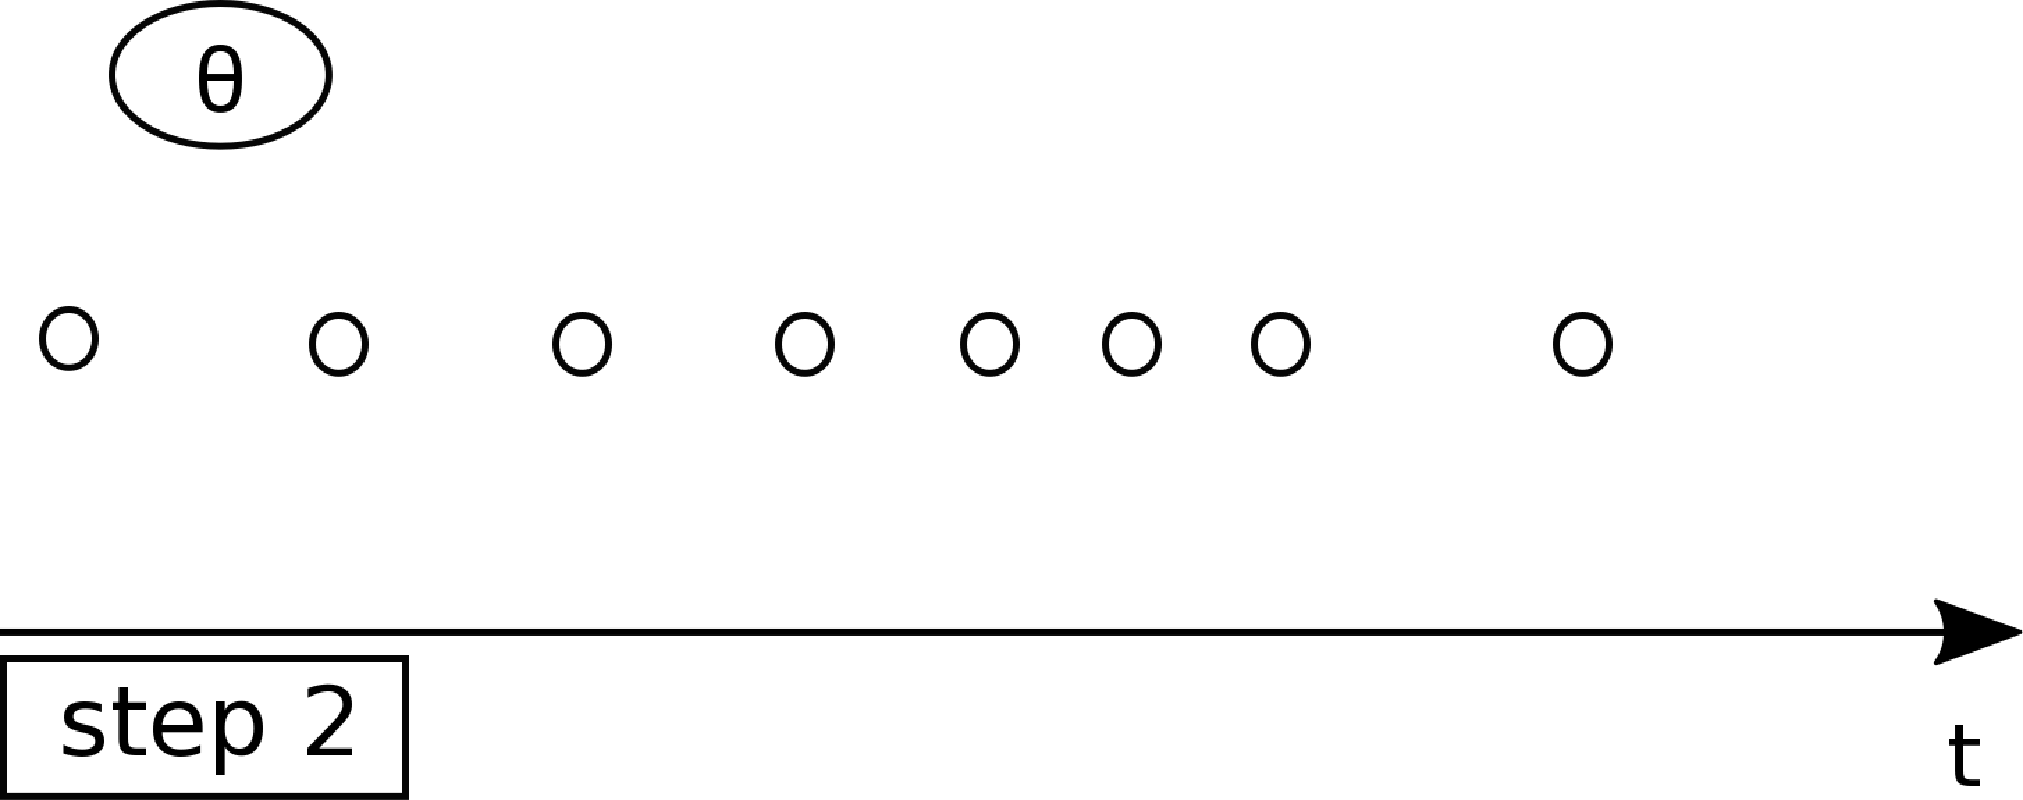
\includegraphics [width=0.70\textwidth, angle=0]{figs/plotn2.png}
    \vspace{-0 in}
  \end{minipage}
  \begin{minipage}[!hp]{0.45\linewidth}
  \centering
    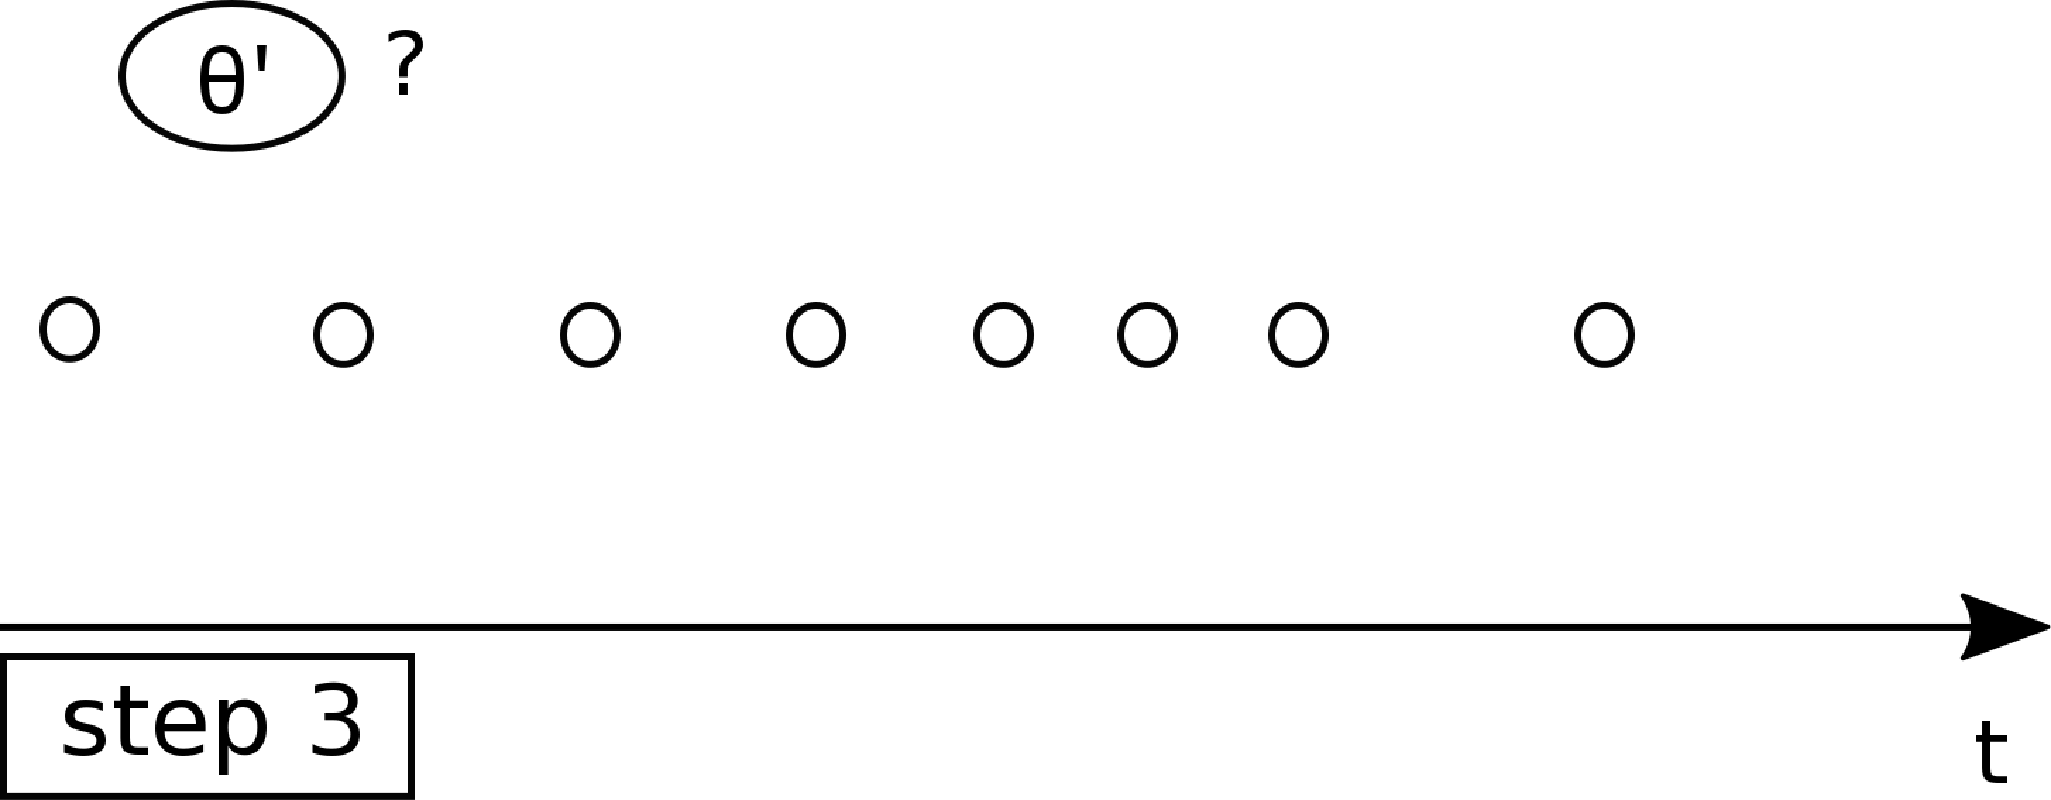
\includegraphics [width=0.70\textwidth, angle=0]{figs/plotn3.png}
    \vspace{-0 in}
  \end{minipage}
  \begin{minipage}[!hp]{0.45\linewidth}
  \centering
    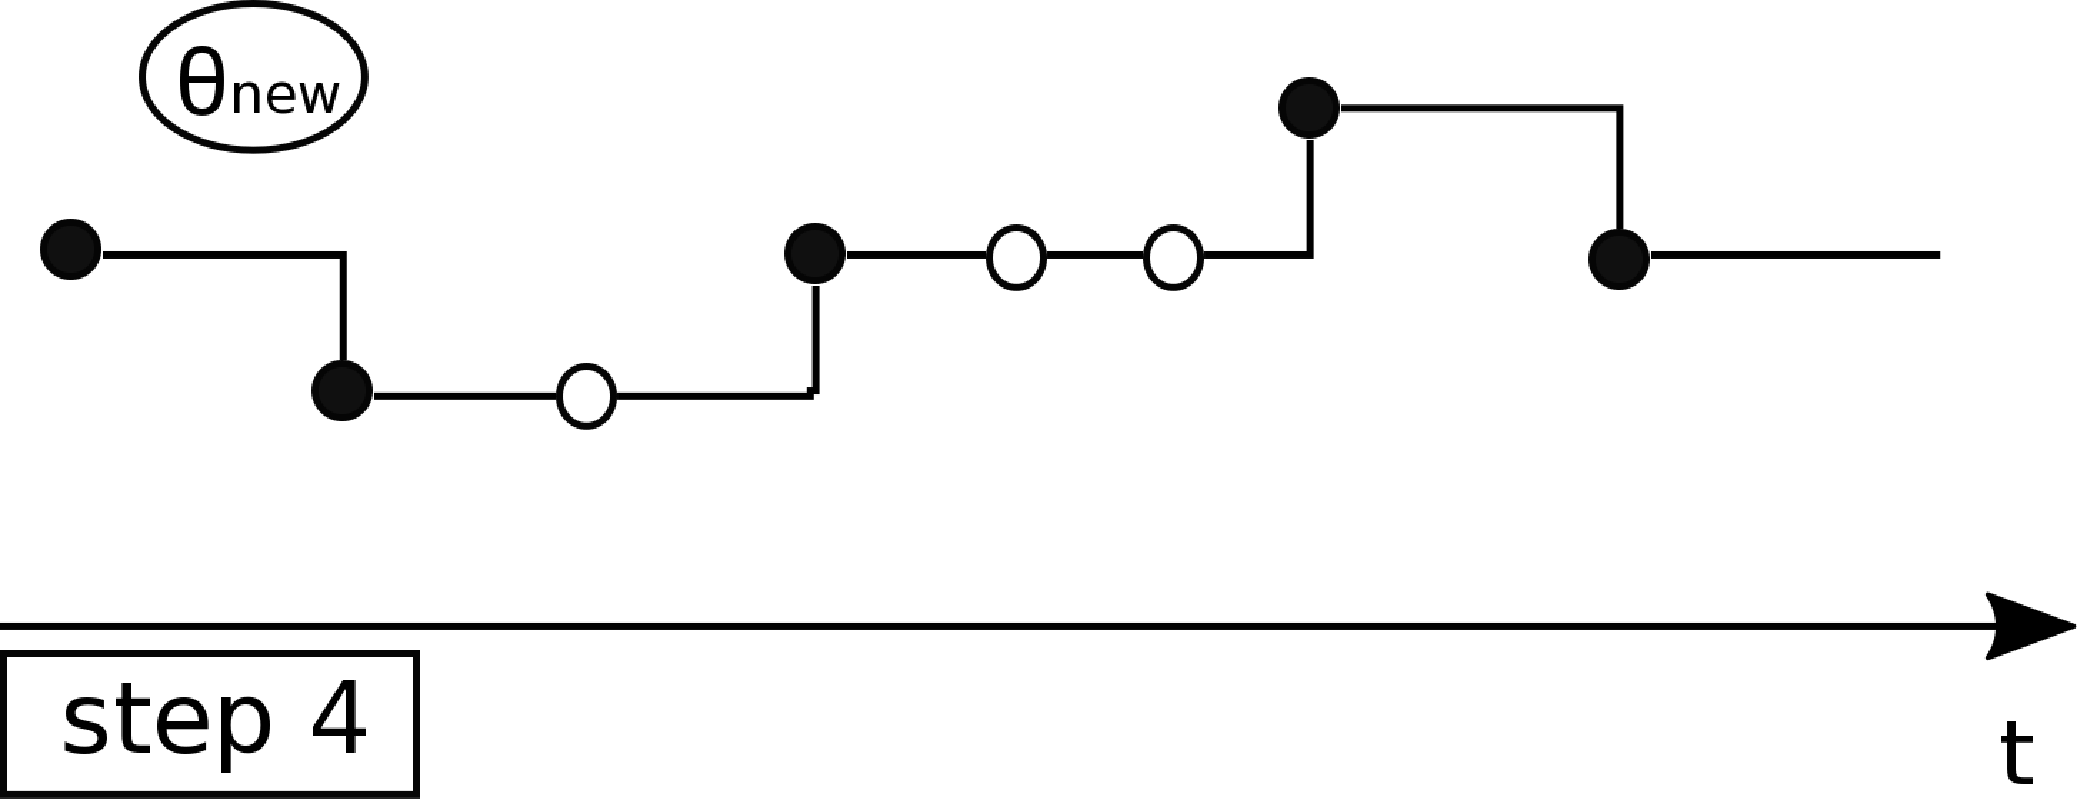
\includegraphics [width=0.70\textwidth, angle=0]{figs/plotn4.png}
    \vspace{-0 in}
  \end{minipage}
  \begin{minipage}[!hp]{0.45\linewidth}
  \centering
    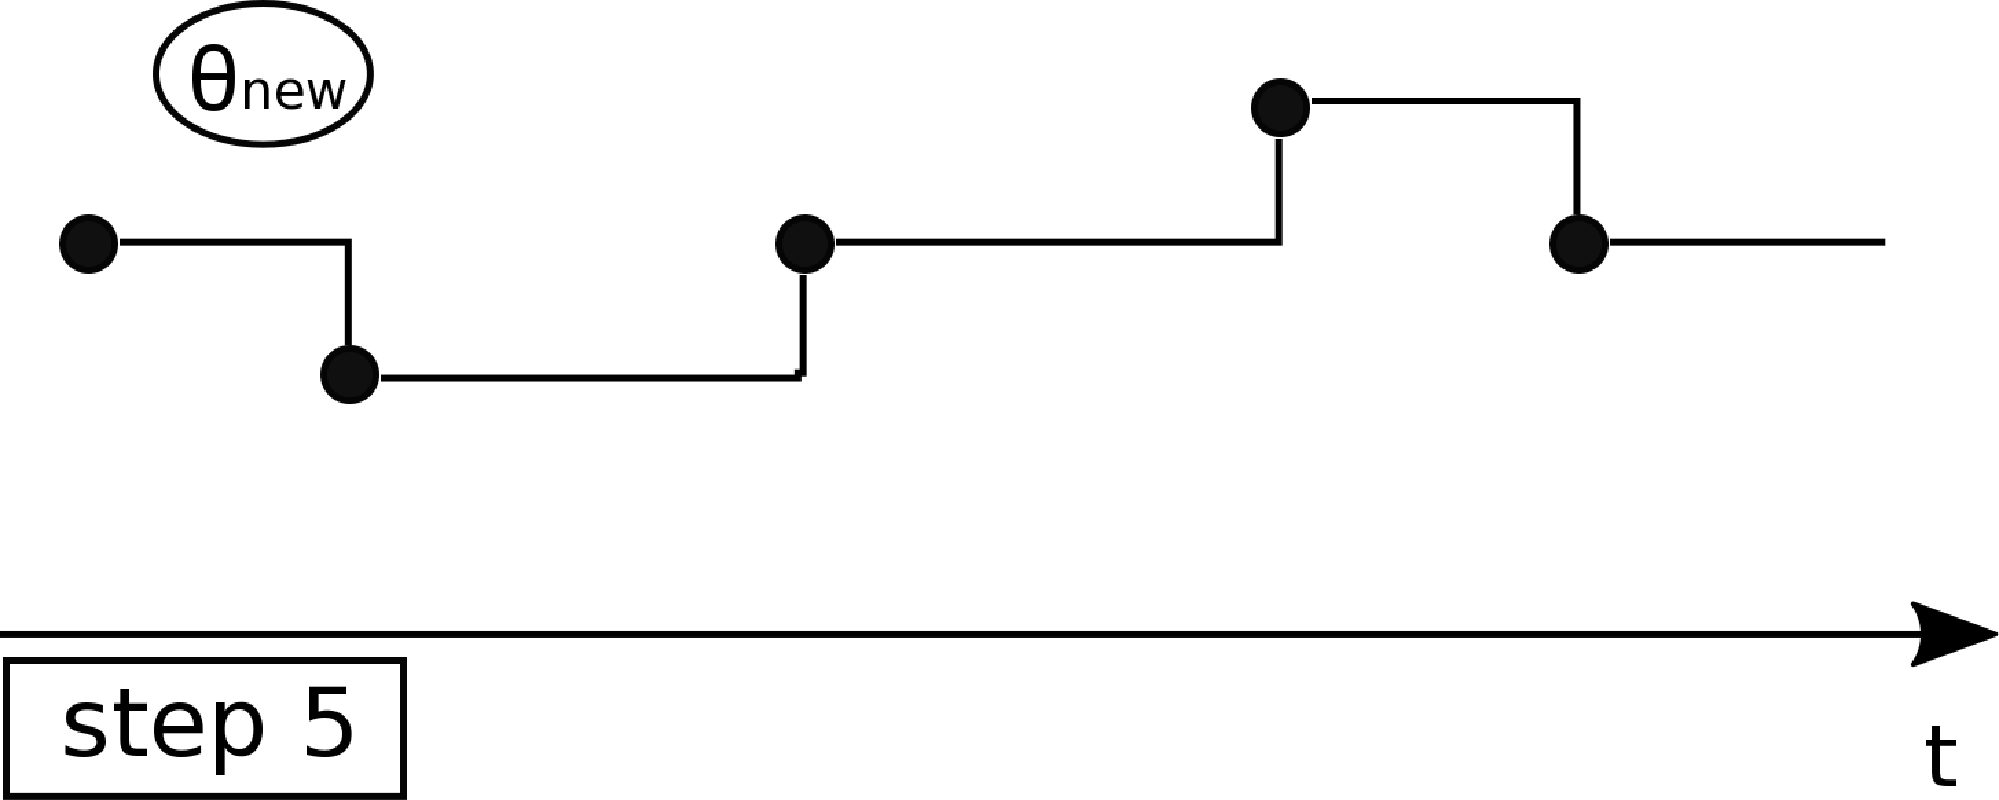
\includegraphics [width=0.70\textwidth, angle=0]{figs/plotn5.png}
    \vspace{-0 in}
  \end{minipage}
    \caption{MH algorithm}

  \end{figure}

\begin{algorithm}[H]
   \caption{MH In Gibbs sampling for MJPs }
   \label{alg:MH In Gibbs}
\begin{algorithmic}
   \STATE {\bfseries Input:} A set of partial and noisy observations $y_{[t_0, t_{N+1})}$, Initial distribution over states $\pi_0$,  Metropolis Hasting proposal $q(. | \theta)$.\\
   The previous MJP path $S(t) = (S, T)$, the previous MJP parameters $\theta$.\\  
      \STATE {\bfseries Output:} A new MJP trajectorie $\tilde{S} (t) = (\tilde{S}, \tilde{T})$, A series of MJP parameters $\tilde{\theta}$.
	\STATE 0: Let $\Omega = h(\theta)$, with $\Omega > max_s{|A_s|}$ using some deterministic function $h$.
	\STATE 1: Sample virtual jumps $U\subset[t_{start}, t_{end}]$ from a Non homogeneous Poisson process with piecewise-constant rate$$R(t) = (\Omega + A_{S(t)}).$$\\Define $W = T \cup U$.
	\STATE 2: Propose $\theta^* \sim q(.| \theta)$.\\
		Accept $\theta^*$ as $\tilde{\theta}$ with probability $\alpha$.
		\begin{align*}
		\alpha &=  1 \wedge \frac{P(W,\theta^*| y)}{P(W, \theta| y)} \frac{q(\theta|\theta^*)}{q(\theta^*|\theta)}\\
		&=  1 \wedge \frac{P(y| W,\theta^*) P(W | \theta^*)p(\theta^*)}{P(y|W, \theta)P(W | \theta)p(\theta)} \frac{q(\theta|\theta^*)}{q(\theta^*|\theta)}.
		\end{align*}
	\STATE 3: Sample a path $\tilde{V}$, from a discret-time Markov chain with $|W| + 1$ steps, using FFBS algorithm. The transition matrix of the Markov chain is $B = (I + \frac{A}{\Omega})$ while the initial distribution over states is $\pi_0$. The likelihood of state $s$ at step $i$ is 
	$$ L_i(s) = P(Y_{[w_i, w_{i + 1})} | S(t) = s \; for\; t \in [w_i, w_{i + 1})) = \prod_{j: t_j \in [w_i, w_{i + 1})}p(y_{t_j} | S(t_j) = s).$$\\
%(i.e. $V(i) \sim P(V |  \theta(i), W(i - 1), y).$) Then delete all the virtual jumps to get $S(i), T(i) .$\\
	\STATE 4: Let $\tilde{T}$ be the set of times in $W$ when the Markov chain changes state. Define $\tilde{S}$ as the corresponding set of state values. Return $(\tilde{S}, \tilde{T}, \tilde{\theta})$.\\
\end{algorithmic}
\end{algorithm}
\label{sec:meth}

\section{Improved Metropolis Hasting for Bayesian Inference using FFBS  within the Gibbs Sampling On MJPs}~
\setlength{\unitlength}{0.8cm}
  \begin{figure}[H]
  \centering
  \begin{minipage}[!hp]{0.45\linewidth}
  \centering
    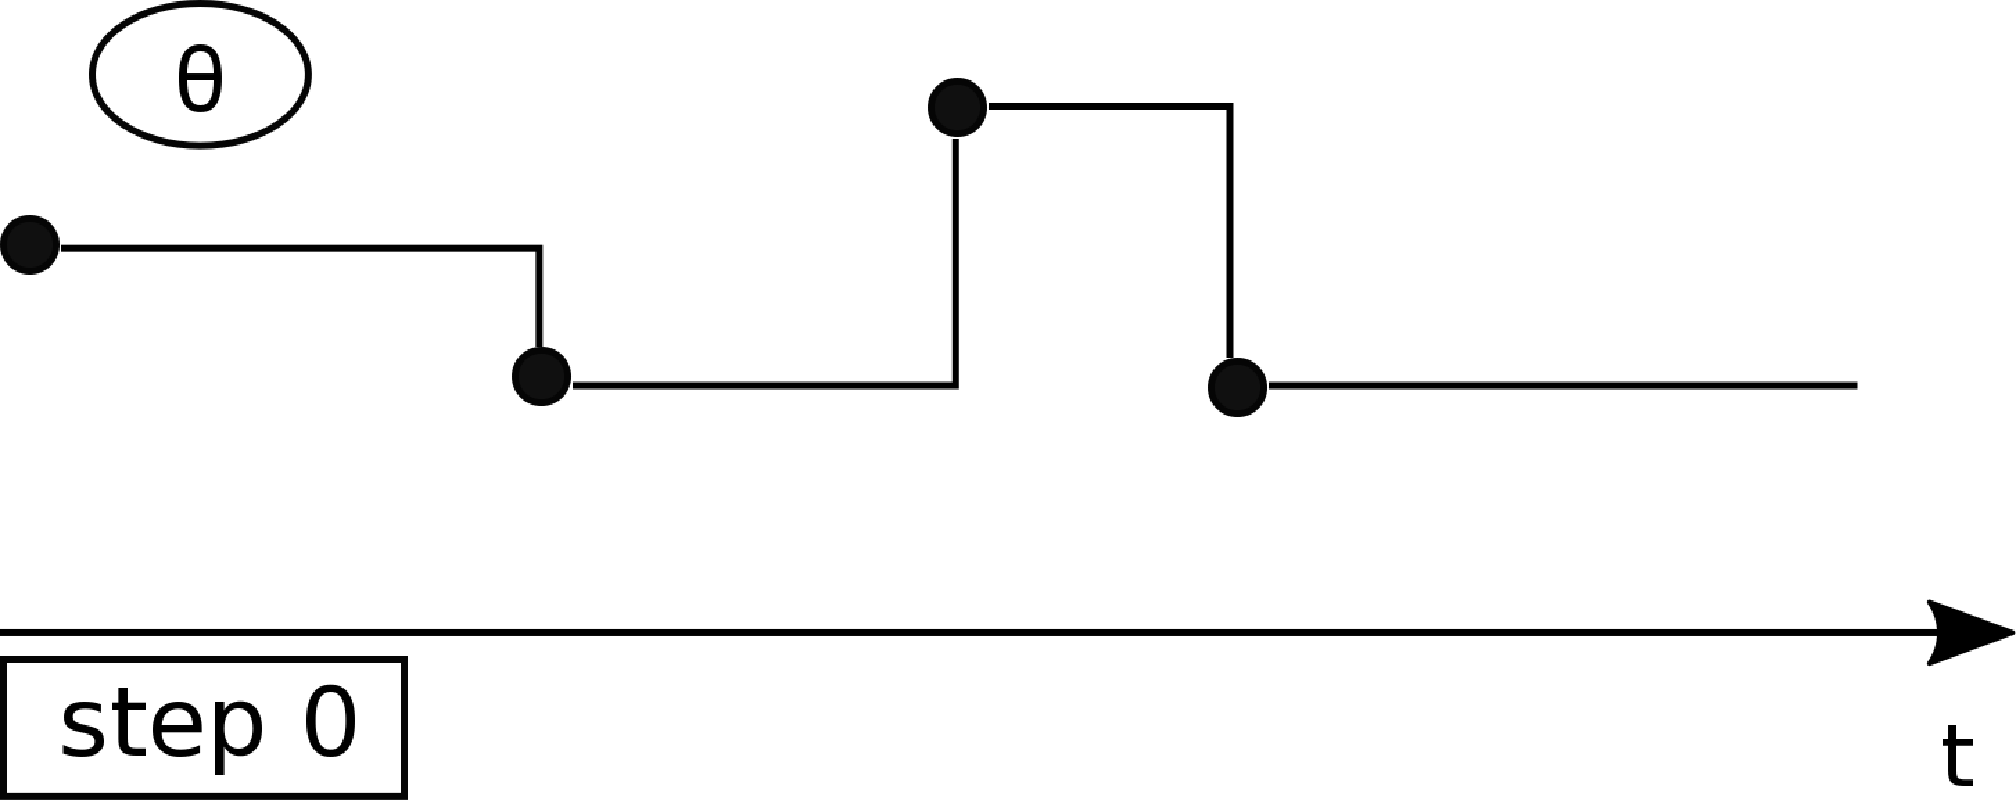
\includegraphics [width=0.70\textwidth, angle=0]{figs/plot0.png}
      \end{minipage}
  \begin{minipage}[hp]{0.45\linewidth}
  \centering
    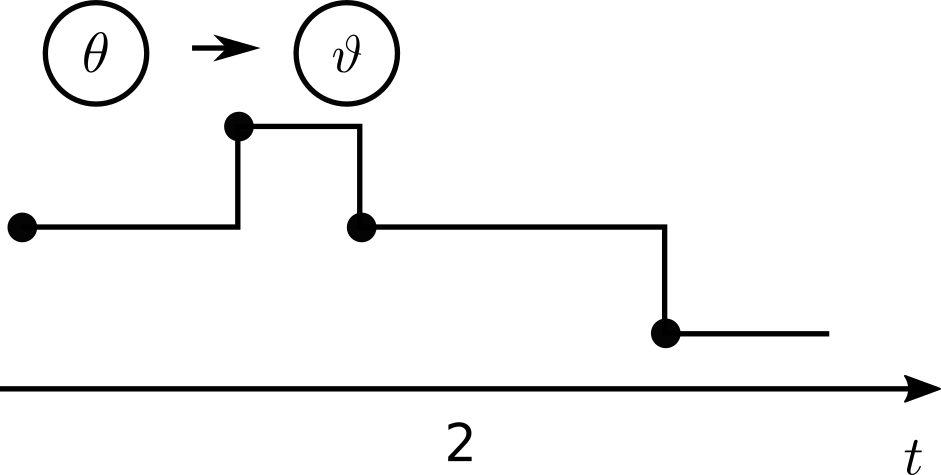
\includegraphics [width=0.70\textwidth, angle=0]{figs/plot1.png}
    \vspace{-0 in}
  \end{minipage}
  \begin{minipage}[hp]{0.45\linewidth}
  \centering
    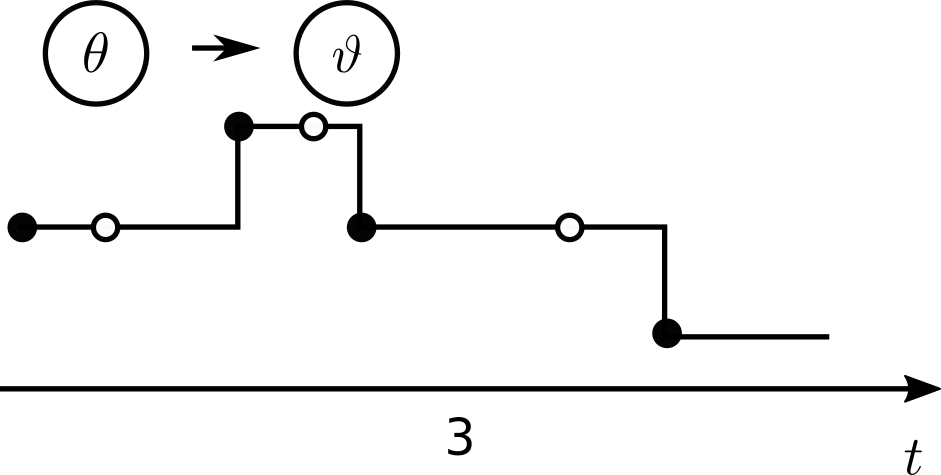
\includegraphics [width=0.70\textwidth, angle=0]{figs/plot2.png}
    \vspace{-0 in}
  \end{minipage}
  \begin{minipage}[hp]{0.45\linewidth}
  \centering
    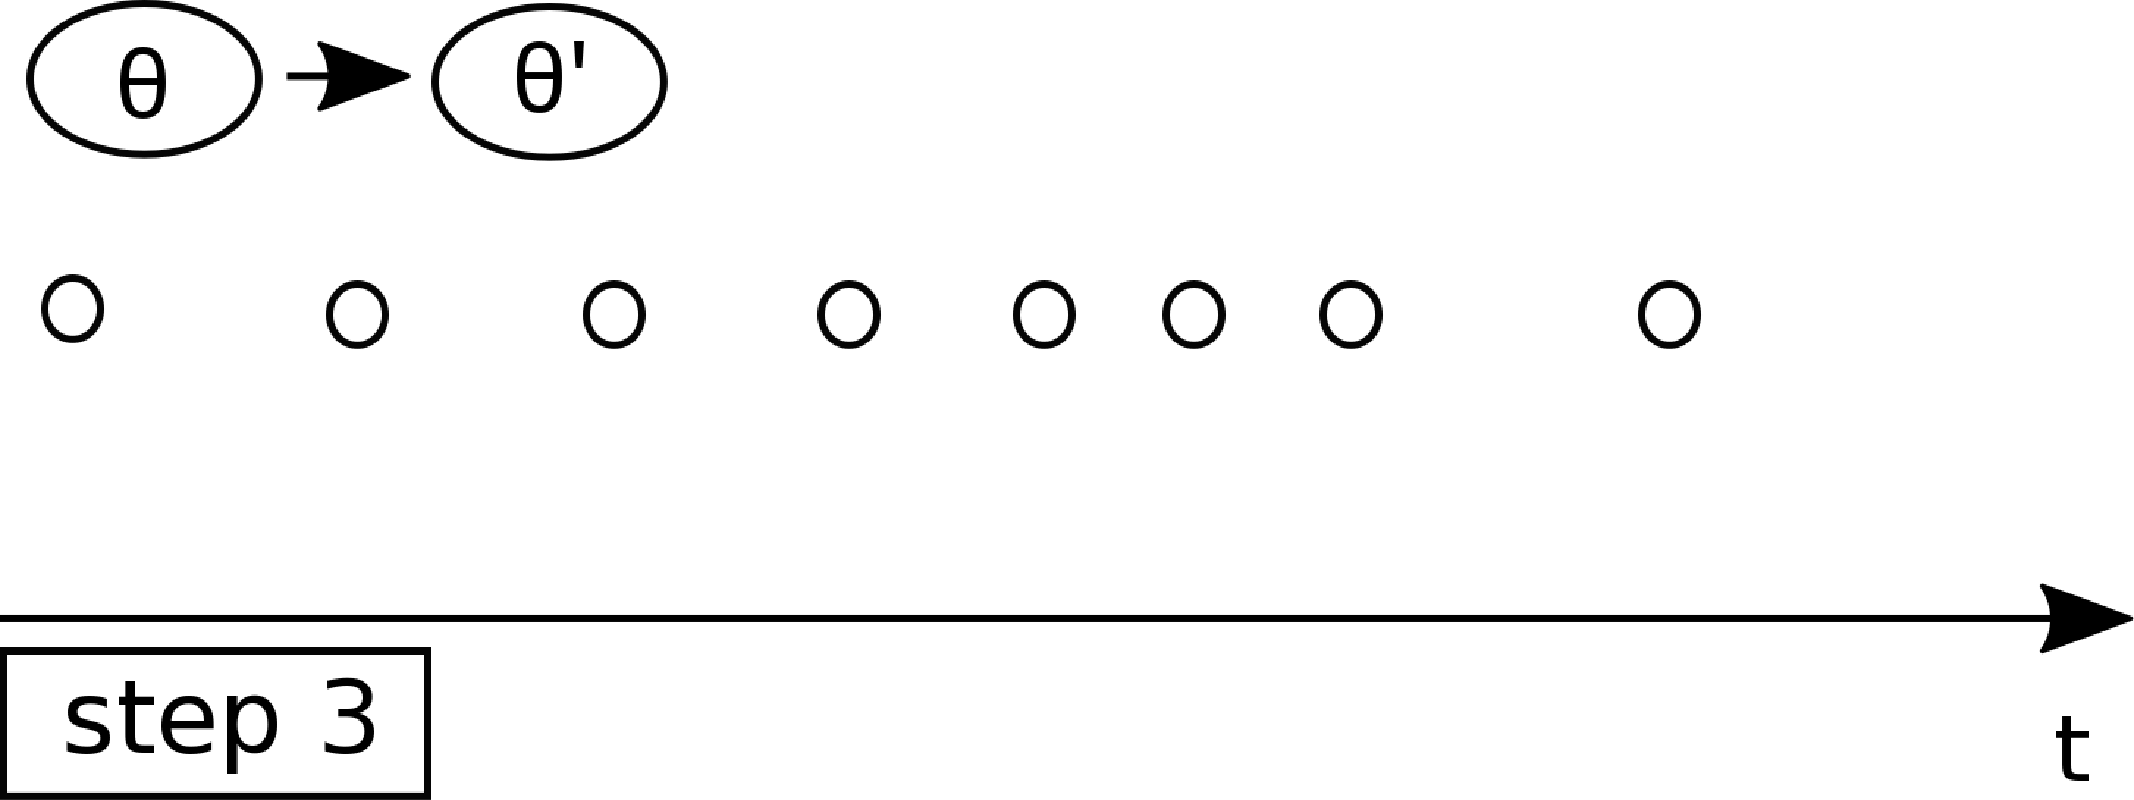
\includegraphics [width=0.70\textwidth, angle=0]{figs/plot3.png}
    \vspace{-0 in}
  \end{minipage}
  \begin{minipage}[hp]{0.45\linewidth}
  \centering
    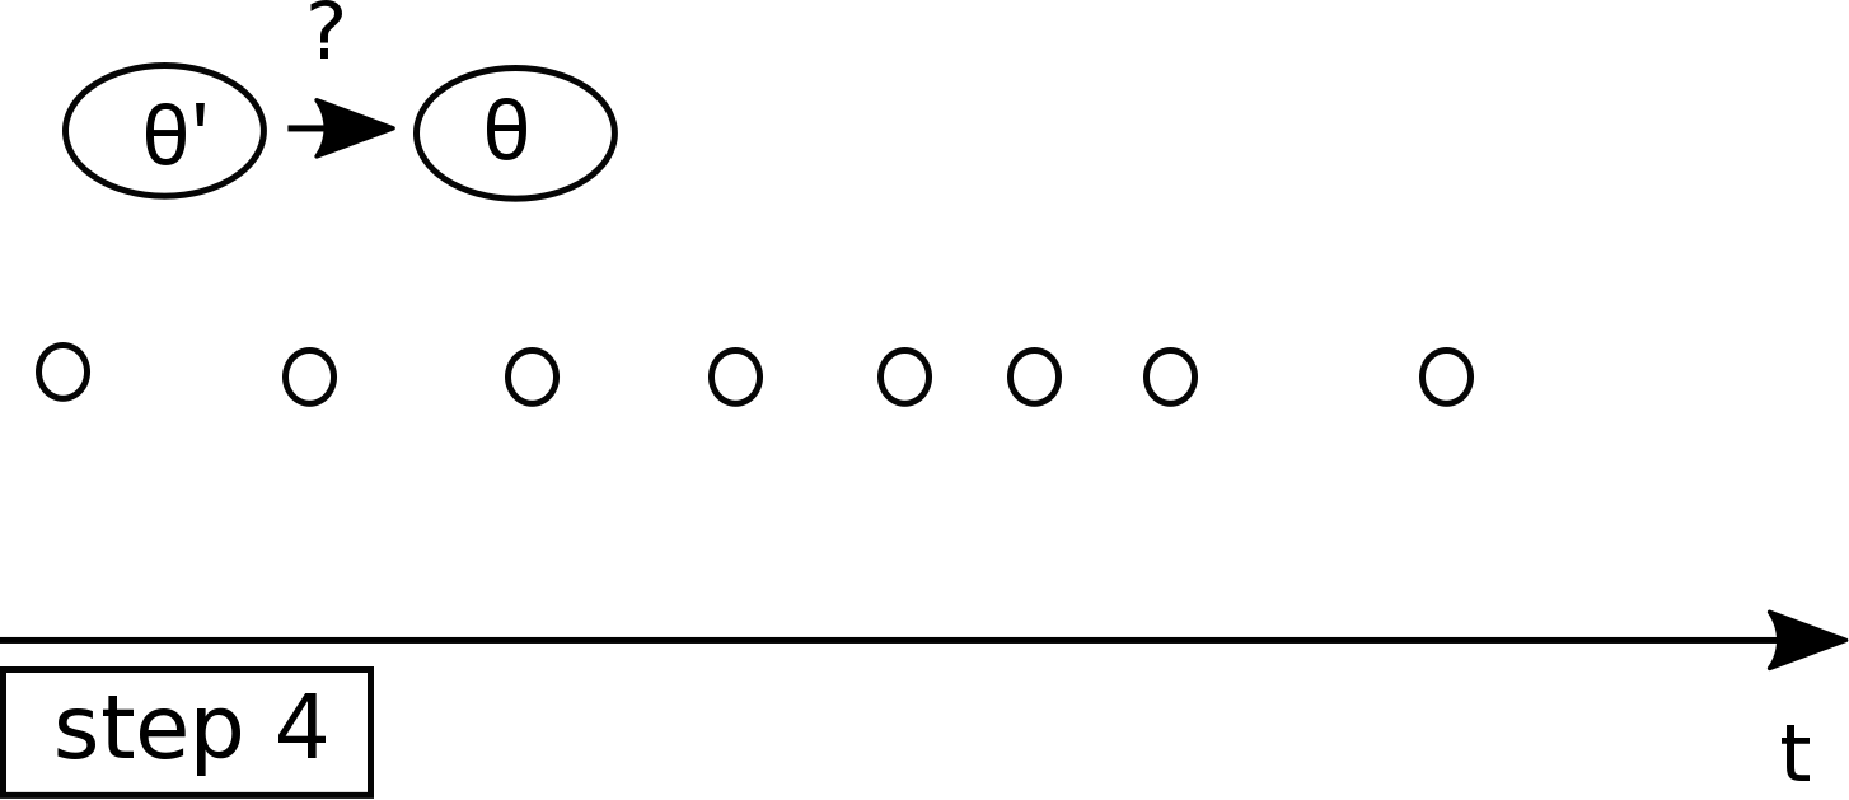
\includegraphics [width=0.70\textwidth, angle=0]{figs/plot4.png}
    \vspace{-0 in}
  \end{minipage}
  \begin{minipage}[hp]{0.45\linewidth}
  \centering
    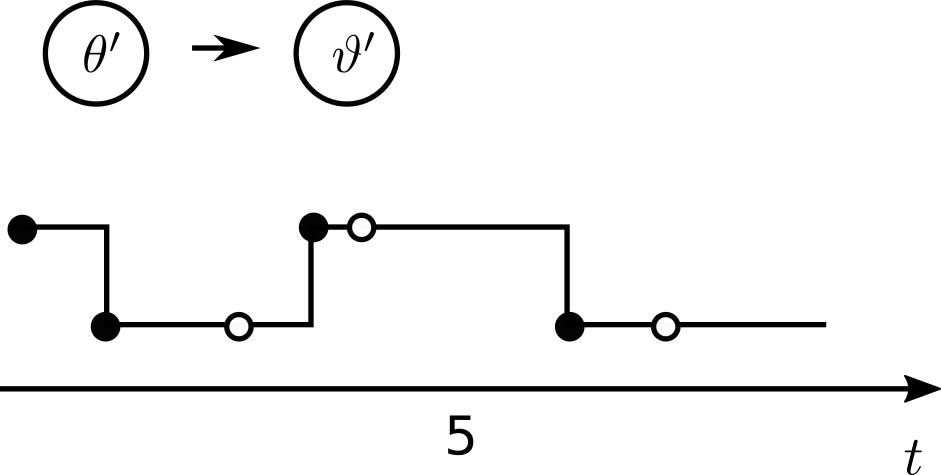
\includegraphics [width=0.70\textwidth, angle=0]{figs/plot5.png}
    \vspace{-0 in}
  \end{minipage}
  \begin{minipage}[hp]{0.45\linewidth}
  \centering
    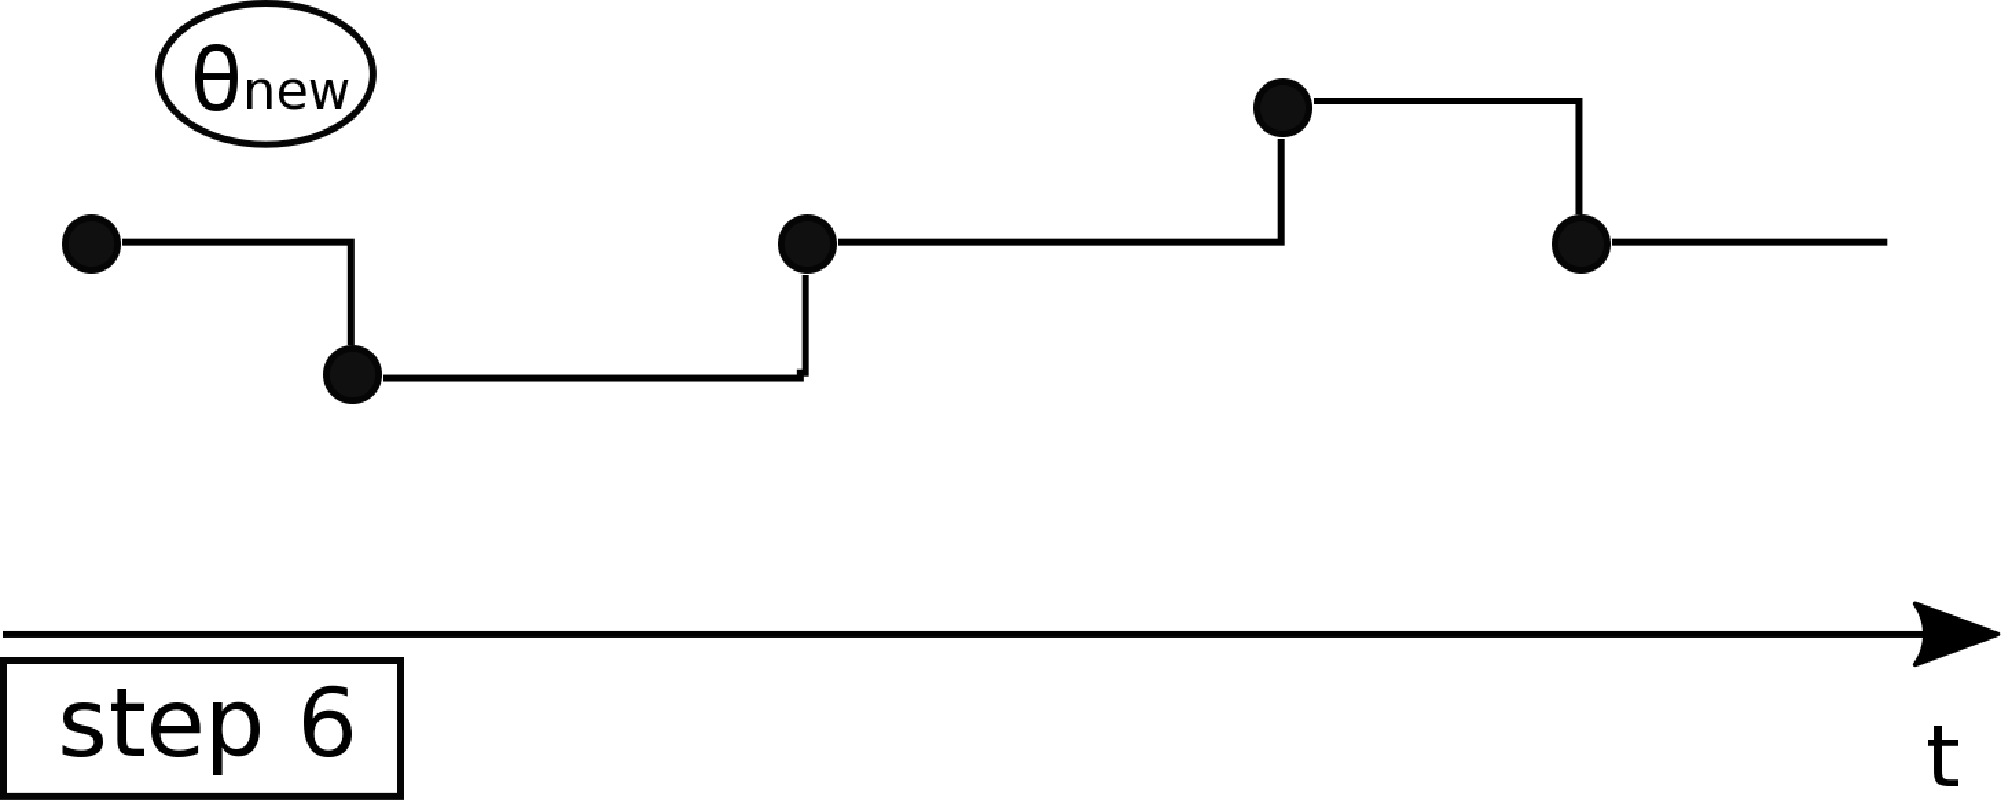
\includegraphics [width=0.70\textwidth, angle=0]{figs/plot6.png}
    \vspace{-0 in}
  \end{minipage}

    \caption{Improved MH algorithm}

  \end{figure}

\begin{algorithm}[H]
   \caption{MH In Gibbs sampling for MJPs }
   \label{alg:MH In Gibbs}
\begin{algorithmic}
   \STATE {\bfseries Input:} A set of partial and noisy observations $y_{[t_0, t_{N+1})}$, Initial distribution over states $\pi_0$,  Metropolis Hasting proposal $q(. | \theta)$.\\
   The previous MJP path $S(t) = (S, T)$, the previous MJP parameters $(\theta)$.\\  
      \STATE {\bfseries Output:} A new MJP trajectorie $\tilde{S} (t) = (\tilde{S}, \tilde{T})$, A series of MJP parameters $\tilde{\theta}$.
	  \STATE 0:  Sample $\theta^* \sim q(.| \theta)$. And let $\Omega = h(\theta) + h(\theta^*)$, with $h(\theta) > max_s{|A_s(\theta)|}$, $h(\theta^*) > max_s{|A_s(\theta^*)|}$ using some deterministic function $h$.
	\STATE 1: Sample virtual jumps $U\subset[t_{start}, t_{end}]$ from a Non homogeneous Poisson process with piecewise-constant rate$$R(t) = (\Omega + A_{S(t)}(\theta)).$$\\Define $W = T \cup U$.
	\STATE 2: Propose $(\theta^*, \theta)$ and accept $\theta^*$ as $\tilde{\theta}$ with probability $\alpha$.
		\begin{align*}
		\alpha &=  1 \wedge \frac{P(W,(\theta^*, \theta)| y)}{P(W, (\theta, \theta^*)| y)}\\
		&=  1 \wedge \frac{P(y| W,\theta^*, \theta) P(W | (\theta^*, \theta))p((\theta^*, \theta))}{P(y| W,(\theta, \theta^*)) P(W | (\theta, \theta^*))p((\theta, \theta^*))}\\
				&=  1 \wedge \frac{P(y| W,\theta^*, \theta)p((\theta^*, \theta))}{P(y| W,(\theta, \theta^*))p((\theta, \theta^*))}.
		\end{align*}
	\STATE 3: Sample a path $\tilde{V}$, from a discret-time Markov chain with $|W| + 1$ steps, using FFBS algorithm. The transition matrix of the Markov chain is $B = (I + \frac{A(\tilde{\theta})}{\Omega})$ while the initial distribution over states is $\pi_0$. The likelihood of state $s$ at step $i$ is 
	$$ L_i(s) = P(Y_{[w_i, w_{i + 1})} | S(t) = s \; for\; t \in [w_i, w_{i + 1})) = \prod_{j: t_j \in [w_i, w_{i + 1})}p(y_{t_j} | S(t_j) = s).$$\\
%(i.e. $V(i) \sim P(V |  \theta(i), W(i - 1), y).$) Then delete all the virtual jumps to get $S(i), T(i) .$\\
	\STATE 4: Let $\tilde{T}$ be the set of times in $W$ when the Markov chain changes state. Define $\tilde{S}$ as the corresponding set of state values. Return $(\tilde{S}, \tilde{T}, \tilde{\theta})$.\\
\end{algorithmic}
\end{algorithm}

\section{Verifications of Algorithm 1}
\label{sec:verify}
Proof of Algorithm 1:\\
\noindent Assume: $S = [S_0,S_1, ...,S_N] \;, T = [T_0, T_1,...,T_N, T_{N+1}(T_{end})]$, and y as observations.\\
In JMLR-2013 Fast MCMC Sampling for MJP and Extensions, the FFBS frame contains $\alpha_t$ as follows.\\
Since after uniformization, the virtual jumps are added.  Then the state process of the trajectory with virtual jumps is just a discrete time markov jump process. The key point is that we need to have $W$ be conditioned, to get the marginal probability $P(y_{[T_0, T_{N + 1})} | \theta, W)$ from FFBS algorithm. \\
\begin{align*}
\alpha^\theta_t(s) = P(S_t = s\;, y_{[T_0, T_t)}, U, T).\\
P(y_{[T_0, T_{N + 1})} | \theta, W) = \sum_{s = 0}^{N-1} \alpha^\theta_N(s) \cdot P(y_{[T_N, T_{N+1})} | S_N = s).\\
P(\theta, W| y) \propto P(\theta, W, y) = P(y| W, \theta) P(W | \theta) P(\theta).
\end{align*}
$P(y|W, \theta)$ is the marginal probability we get after Forward Filtering Algorithm and the $P(W | \theta)$ is the probability density for the $poisson(\Omega)$, because of the uniformization procedure.
Let denote the kernel for (a), (b) and (c) as  $\kappa_1(\theta^*| \theta, W, T, S, y)$ , $\kappa_2(S^*, T^*|S, T, W, \theta^*, y)$ and $\kappa_3(W^*| S^*, T^*, \theta^*, y)$.\\
For Step (a) $\kappa_1(\theta^*| \theta, W, T, S)$:\\
 \begin{align*} 
P((W, T, S, \theta) \rightarrow (W, T, S, \theta^*)) P(\theta, W | y) &=  P(\theta^*, W | y)q(\theta | \theta^*)
 \wedge P(\theta, W|y) q(\theta^*| \theta) \\&= P((W, T, S,\theta^*) \rightarrow (W, T, S,\theta)) P(\theta^*, W | y).\\
\end{align*}
Thus, $  \int ab \kappa_1(\theta^*| \theta) P(\theta, W|y) d\theta = P(\theta^*, W |y). $\\
So the stationary distribution of $\kappa_1$ is $P(\theta, W | y)$.\\
Step (b) $\kappa_2(S^*, T^*|S, T, W, \theta^*, y)$: \\ 
Step(b) is the same as Fast MJPs Gibbs sampling scheme.   \\
\begin{align*}
((S, T, \theta, W) \rightarrow (S^*, T^*,\theta, W)|  y) = P(V^* | W, \theta, y) = P(V^* | W, \theta, y) / P(W, \theta, y) \end{align*}
\begin{align*}
P((S, T) \rightarrow (S^*, T^*)| W, \theta, y) P(S, T| W, \theta, y) &= P(V^* | W, \theta, y)P(V | W, \theta, y) \\&= P((S^*, T^*) \rightarrow (S, T)| W, \theta, y) P(S^*, T^*| W, \theta, y)
\end{align*}
\\So the stationary distribution of $\kappa_2(S^*, T^*| S,T,  W, y)$ is $P(S, T | W, \theta, y).$
Now, let's consider $\kappa_2 \circ \kappa_1(S^*, T^*, \theta^* | S, T, \theta, y, W)$.\\
\begin{align*}
((S, T, \theta, W) \rightarrow (S^*, T^*, \theta^*, W)|  y) = P((W, T, S, \theta) \rightarrow (W, T, S, \theta^*)) P((S, T, \theta^*.W) \rightarrow (S^*, T^*, \theta^*, W)| y) .
\end{align*}
The stationary distribution of $\kappa_1(S^*, T^*, U^*|S, T, U)$ is $P(S,T,U| \theta, y).$ And the stationary distribution of $\kappa_2(U^*| U)$ is $P(U| S, T, \theta, y).$ \\
\begin{align*}
&P((S, T, \theta, W) \rightarrow (S^*, T^*, \theta^*, W)|  y) P(S,T,\theta | W, y) \\&= P((W, T, S, \theta) \rightarrow (W, T, S, \theta^*))\cdot P(\theta|W,y) \cdot P((S, T, \theta^*.W) \rightarrow (S^*, T^*, \theta^*, W)| y) P(S, T | \theta , W, y) \\&=P((W, T, S, \theta^*) \rightarrow (W, T, S, \theta))\cdot P(\theta^*|W,y) \cdot P((S^*, T^*, \theta^*.W) \rightarrow (S, T, \theta^*, W)| y) P(S^*, T^* | \theta , W, y) \\&=P((S^*, T^*, \theta^*, W) \rightarrow (S, T, \theta, W)|  y) P(S,T,\theta | W, y).
\end{align*}
So the stationary distribution of $\kappa_2 \circ \kappa_1$ is $P(S, T,\theta| W,y).$\\
Obviously, $\kappa_3(W^*| W, S^*, T^*, \theta^*, y)$ has $P(W| S^*, T^*, \theta^*,y)$ as stationary distribution.\\
Therefore, $\int \kappa_3(W^*| W, S^*, T^*, \theta^*, y) P(W,S^*, T^*, \theta^*|y ) dW= P(W^*,S^*, T^*, \theta^*|y )$.\\
Thus, $\int \kappa_3 \cdot (\int \kappa_2 \circ \kappa_1\cdot P(W,S, T, \theta | y) d\theta dS dT)dW = \int \kappa_3 P(W,S^*, T^*, \theta^*|y )dW = P(W^*,S^*, T^*, \theta^*|y )$.\\
So the stationary distribution of $\kappa_3 \circ \kappa_2 \circ \kappa_1$ is $P(W^*,S^*, T^*, \theta^*|y )$.
%\end{proof}

\section{Verifications of Algorithm 2}
\label{sec:verify}
Proof:
Our state is $(W, S, T, \theta, \theta^*)$. 
\begin{align*}
 p(y, W, S, T, \theta, \theta^*) &= p(\theta) q(\theta^* | \theta) P(S,T| \theta, \theta^*) P(W| S, T, \theta, \theta^*)P(y | S, T, \theta, \theta^*)\\
 &=p(\theta) q(\theta^* | \theta) P(S,T| \theta) P(W| S, T, \theta, \theta^*)P(y | S, T).
\end{align*}
The marginal distribution of $(y, S, T, \theta, \theta^*)$ and $(y, S, T, \theta)$ as follows.\\
\begin{align*}
 p(y, S, T, \theta, \theta^*) &= p(\theta) q(\theta^* | \theta) P(S,T| \theta, \theta^*)P(y | S, T, \theta, \theta^*)\\
 &=P(y, S, T, \theta) q(\theta^* | \theta).
\end{align*}
\begin{align*}
 p(y, S, T, \theta) &= p(\theta)P(S,T| \theta)P(y | S, T, \theta).
\end{align*}
So the conditional distribution over $\theta^*$ given $(y, S, T, \theta)$ is $q(\theta^* | \theta)$. And the conditional distribution over W given $(y, S, T, \theta, \theta^*)$  is $P(W | S, T, \theta, \theta^*)$, which is actually the distribution of Non Homogeneous Poisson Process with piecewise constant rate $h(\theta) + h(\theta^*) - A_{S(t)}(\theta)$.\\
Thus the Step 1 + Step 2 is actually equivalent to sampling from the conditional distribution $P(\theta^* , W| S, T, \theta, y)$.\\
The Step 3 + Step 4 satisfy the detailed balance condition. The reason is as follows.
\begin{align*}
&P((W, S, T, (\theta, \theta^*)) \rightarrow (W, S^*, T^*, (\theta^*, \theta))) P(S,T, (\theta, \theta^*) | W, y)\\
&= (1 \wedge \frac{P((\theta^*,\theta) | W, y)}{P((\theta,\theta^*) | W, y)})P(S^*, T^* | W, (\theta^*, \theta), y)P(S, T | W, (\theta, \theta^*), y)P((\theta, \theta^*) | W, y)\\
&= P((W, S^*, T^*, (\theta^*, \theta)) \rightarrow (W, S, T, (\theta, \theta^*))) P(S^*,T^*, (\theta^*, \theta) | W, y)
\end{align*} 
Therefore the stationary distribution of this MCMC sampler is $P(W, S, T, (\theta, \theta^*) | y)$. Thus the stationary distribution of $(S, T, \theta)$ is the corresponding marginal distribution $P(S, T, \theta | y)$.  

\section{Generic Exponential Model}~
\begin{algorithm}[!ht]
   \caption{Generic Gibbs sampling for MJPs for Gamma priors}
   \label{alg:Generic Gibbs}
\begin{algorithmic}
   \STATE {\bfseries Input:} observations $y_{[t_0, t_{k+1})}$
   \STATE Initialize, $i = 0$
   \\ (a) Set $\alpha(0), \beta(0)$ arbitrarily and set current trajectory $[S,T](0)$ arbitrarily.\\
	(b) Uniformize $[S,T](0)$, to get virtual jumps $U$.
   \REPEAT
   \FOR{$i=1$ {\bfseries to} $N$}
	\STATE (a) Sample $U(i) \sim P( U | \beta(i - 1), \alpha(i - 1), S(i - 1), T(i - 1), y)$.\\	
	\STATE (b) Use FFBS algorithm to  sample states given all the jump times(both true jumps and virtual jumps).
(i.e. $V(i) \sim P(V |  \beta(i - 1), \alpha(i - 1), W(i ), y).$) Then delete all the virtual jumps to get $S(i), T(i) .$\\
	\STATE (c) Propose $\beta^* \sim q(.| \beta(i -1))$.\\
	  Set $\beta(i) = \beta^*$, with probability $P_{acc} = 1 \wedge \frac{P(\beta^* |S(i), T(i))}{P(\beta(i - 1) |S(i), T(i))} \frac{q(\beta(i - 1)|\beta^*)}{q(\beta^*|\beta(i - 1))}$;\\Otherwise set $\beta(i) = \beta(i-1)$.\\	  
	\STATE (d) Sample $\alpha(i) \sim P(. | \beta(i), S(i), T(i), y)$.\\ It is a $Gamma(\mu + N, \lambda + \sum_{0}^NF_{S_i}(\beta)(t_{i + 1} - t_i))$ distribution actually.\\
   \ENDFOR
   \UNTIL{$ i = N$ }
\end{algorithmic}
\end{algorithm}
  \begin{figure}[H]
  \centering
  \begin{minipage}[!hp]{0.45\linewidth}
  \centering
    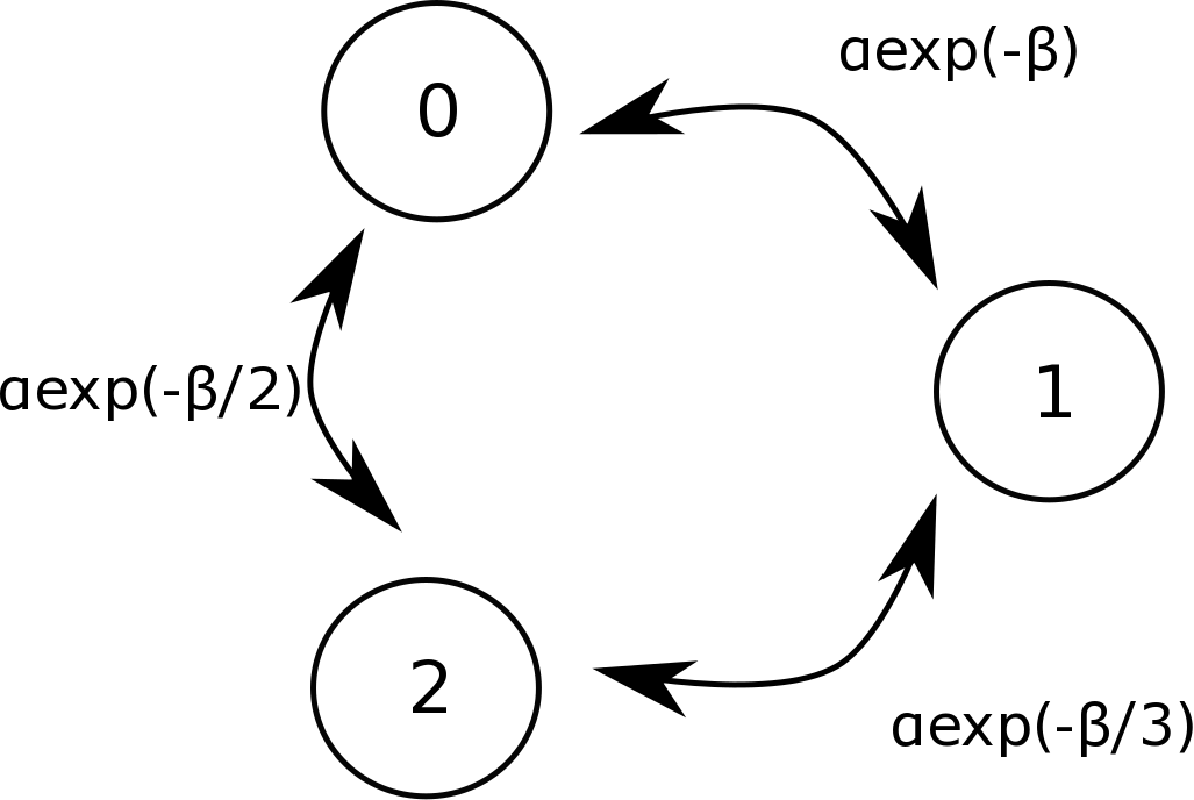
\includegraphics [width=0.70\textwidth, angle=0]{figs/expplot.png}
      \end{minipage}
    \caption{exp model}
  \end{figure}

\noindent Assume: $S = [S_0,S_1, ...,S_N] \;, T = [t_0(t_{start}), t_1,...,t_N, t_{N+1}(t_{end})]$, and y as observations.\\
We consider a specific structure of rate matrix $A$. $A_{ij} = \alpha f_{ij}(\beta), \; i \neq j$. $A_{ii} = -\sum_{j \neq i} A_{ij}$. $0 \leq f_{ij} \leq 1$. Denote $F_i(\beta) = \sum_{j \neq i} f_{ij}(\beta)$.\\
\begin{align*}
P(s_0, S, T | \alpha, \beta) &= \pi_0(s_0)\prod_{i = 1}^N A_{S_{i - 1}S_i} \exp(- \int_{t_{start}}^{t_{end}} |A_{S(t)}| dt)\\
&= \pi_0(s_0) \alpha^N \prod_{i = 1}^N f_{S_{i - 1}S_i} \exp(-\alpha  \sum_{i = 0}^{N} F_{S_i}(\beta)(t_{i + 1} - t_i))\\
\end{align*}
We can assume the prior distributions of $\alpha, \beta$ are $p_1(\alpha)$ and $p_2(\beta)$.\\
Then the posterior distribution of parameters $\alpha, \beta$ will be as follows.\\
\begin{align*}
P(\alpha, \beta | s_0, S, T ) \propto \alpha^N \prod_{i = 1}^N f_{S_{i - 1}S_i} \exp(-\alpha  \sum_{i = 0}^{N} F_{S_i}(\beta)(t_{i + 1} - t_i)) p_1(\alpha)p_2(\beta)\\
\end{align*}
If we assume the priors of $\alpha$, $\beta$ are $Gamma(\mu, \lambda)$, $Gamma(\omega, \theta)$, then the posterior will have a simper form as follows. 
\begin{align*}
P(\alpha, \beta | s_0, S, T ) = C \alpha^{\mu + N - 1}\exp(-\alpha (\lambda + \sum_{i = 0}^{N} F_{S_i}(\beta)(t_{i + 1} - t_i))) \prod_{i = 1}^N f_{S_{i - 1}S_i}  \beta ^{\omega - 1} \exp(-\theta \beta)\\
\end{align*}
We notice that given $\beta,\; S,\; T$, $\alpha$ is distributed as a $Gamma$ distribution.\\
$\alpha | \beta, S, T, y  = \alpha | \beta, S, T \sim Gamma(\mu + N, \lambda + \sum_{0}^NF_{S_i}(\beta)(t_{i + 1} - t_i))$.\\
There is no conjugate distribution to sample $\beta \sim P(\beta| s_0, S, T)$. We will have to use Metropolis Hasting within Gibbs to sample $\beta$. The target distribution is the following one.
$$ P(\beta | S, T) = C \frac{\prod_{i = 1}^N f_{S_{i -1}S_i}(\beta)\beta^{\omega - 1} \exp(-\theta \beta)}{(\lambda + \sum_{i = 0}^{N} F_{S_i}(\beta)(t_{i + 1} - t_i))^{\mu + N}}.$$
Such doubling might slow the mixing of the Markov chain. We can apply our Metropolis Hasting algorithm on this model.
\subsection{Experiments}
In the following, we evaluate a Python implementation of our algorithms compared to other exact samplers which include Gibbs sampler and Particle MCMC sampler. We consider one special case when $f_{ij}(\beta) = \exp(-\beta / (i + j))$. We consider three different dimensions which are 3, 5, and 10 and three different k which are 1.5, 2, and 3. We generated random parameters $\alpha$, $\beta$ from prior distributions ($Gamma(3,2), Gamma(5, 2)$), and used these parameters to construct the transition matrix A. Then we generate an MJP trajectory with a uniform initial distribution over states and the transition matrix A. The state of this MJP trajectory was observed via a Normal distribution with mean equal to the value of state and variance 1, and the proposal kernel is a lognormal distribution with location parameter $\log(\theta_{old})$ and scale parameter$\sigma$. Posterior samples given the observations were produced by a Python implementation of our algorithm. 100 MCMC runs were performed, each run consisting of 10000 iterations except for Particle MCMC algorithm. For Particle MCMC, each run consists 3000 iterations while the number of particles can be 5, 10 or 20. For each run, the acceptance rates as well as the time spent was calculated, and effective sample sizes (ESSs) of MCMC sampling parameters) were calculated using R-CODA (Plummer et al., 2006). The overall ESS per unit time of a run is defined to be the mean ESS per unit time across all these ESSs per unit time.\\
Figure 1, 2 and 3 plot the overall  ESS per unit time against the variance of the proposal kernel per run, for different methods and different scaling parameters k($k = 1.5, 2, 3$) and different dimensions($p = 3, 5, 10$), where the  $\Omega = k \max(\Omega_{old}, \Omega_{new})$ when $k < 2$, or $\Omega = k (\Omega_{old} + \Omega_{new})$ when $k \leq 2$. We see that the improved MH algorithm is more efficient in these cases with respect to the overall ESS per unit time. We also see that increase the scaling parameter will decrease the efficiency of the improved MH algorithm respect to overall ESS per unit time, when $k > 2$. If we set $\Omega = 1.5 \max(\Omega_{old}, \Omega_{new})$, the performance of the improved MH will not be as good as the case we set $\Omega = 2(\Omega_{old} + \Omega_{new})$ when the proposal log variance is large.\\
Figure 4 shows the initial burn-in of a sampler with this setting for different initializations. The vertical axis shows the number of state transitions in the MJP trajectory of each iteration. This quantity quickly reaches its equilibrium value within a few iterations.\\

Figure 5 plot ESS per unit time as observation interval and the number of observations both increase when the dimension is $3$ and the scaling parameter k is $2$. Gibbs sampler decreases faster than Metropolis Hasting Method, due to the doubling of MJP paths and the parameters. \\

Figure 6 plot ESS per unit time as observation interval increases with number of observations fixed, when the dimension is $3$ and the scaling parameter k is $2$.Gibbs sampler decreases faster than Metropolis Hasting Method, due to the doubling of MJP paths and the parameters. In addition Gibbs sampler decreases even more faster than previous case when the number of observations is not fixed. \\

Figure 7 plots ESS plots the overall  acceptance rate against the log variance of the proposal kernel per run for dimension $3$. 


  \begin{figure}%[b]
  \centering
  \begin{minipage}[!hp]{0.45\linewidth}
  \centering
    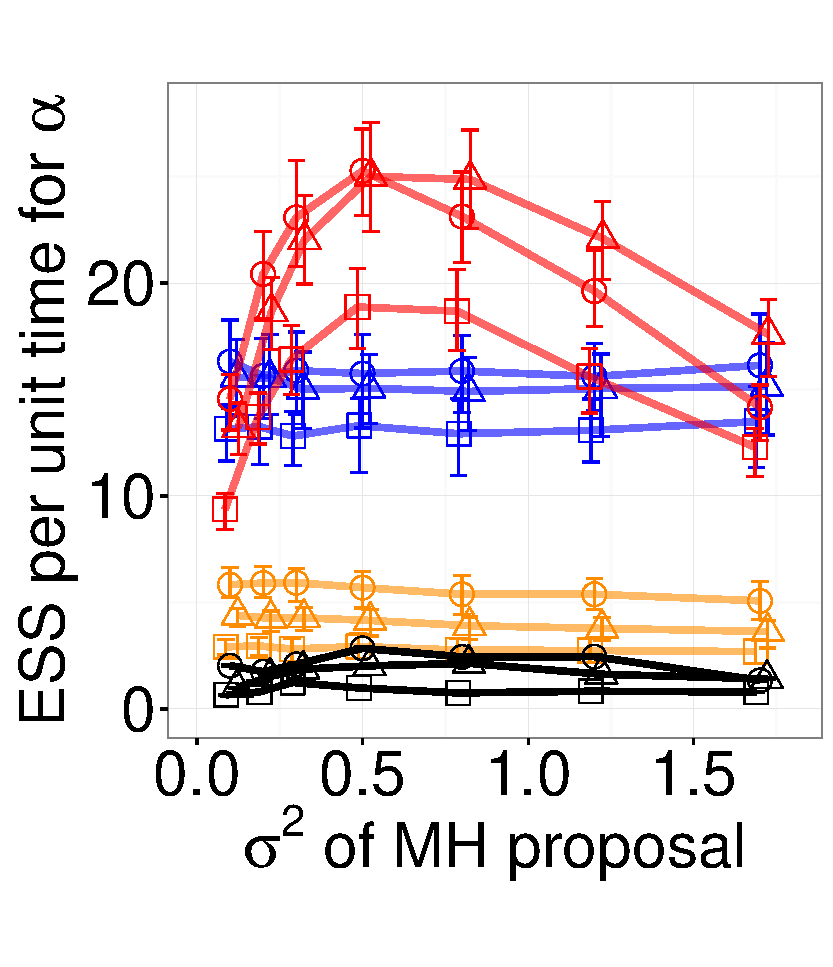
\includegraphics [width=0.70\textwidth, angle=0]{figs/exp_3_alpha.pdf}
      \end{minipage}
  \begin{minipage}[hp]{0.45\linewidth}
  \centering
    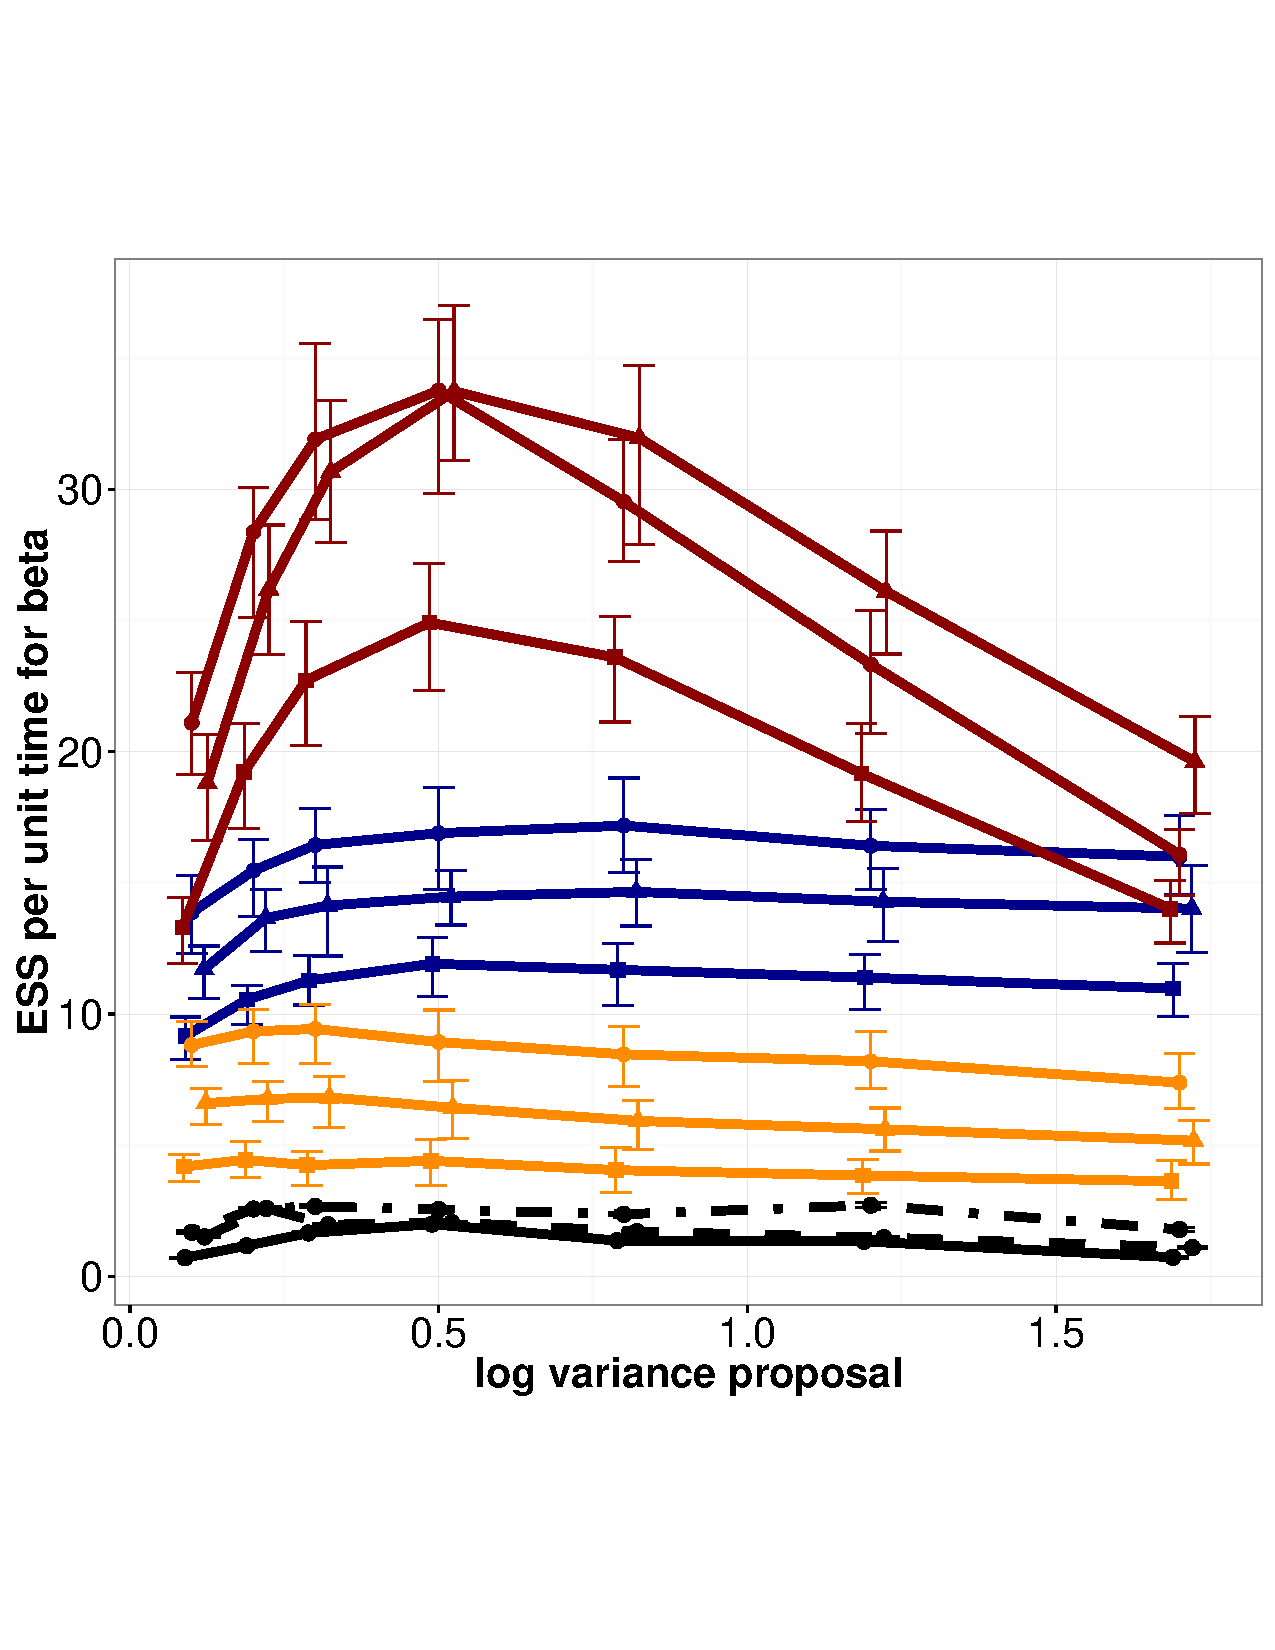
\includegraphics [width=0.70\textwidth, angle=0]{figs/exp_3_beta.pdf}
    \vspace{-0 in}
%    \caption{ESS/sec for exp model (beta, dim 3)}
     \label{fig:ESS_EXP_D3}
  \end{minipage}
    \caption{ESS/sec for exp model (dim 3). The left is for $\alpha$, and the right is for $\beta$.}
  \end{figure}
  \begin{figure}[H]
  \centering
  \begin{minipage}[hp]{0.45\linewidth}
  \centering
    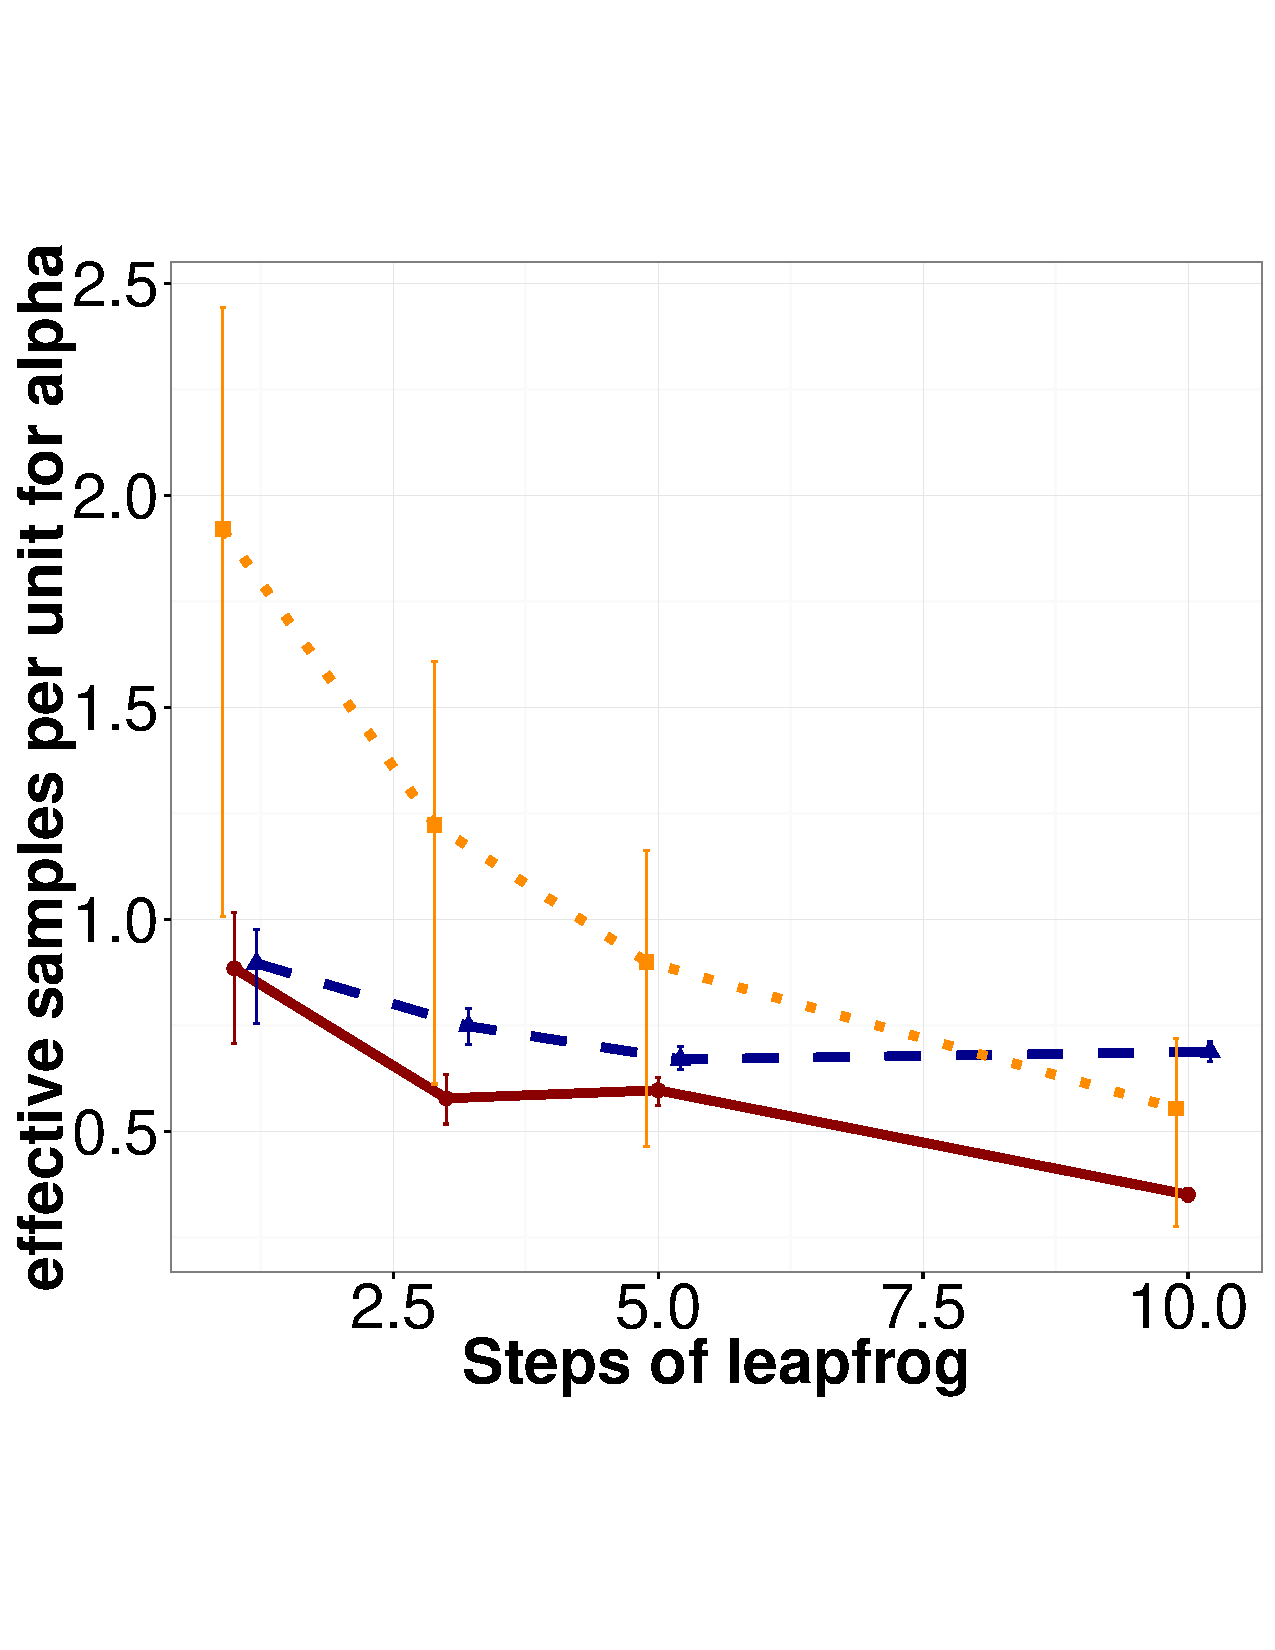
\includegraphics [width=0.70\textwidth, angle=0]{figs/h_alpha.pdf}
      \end{minipage}
  \begin{minipage}[hp]{0.45\linewidth}
  \centering
    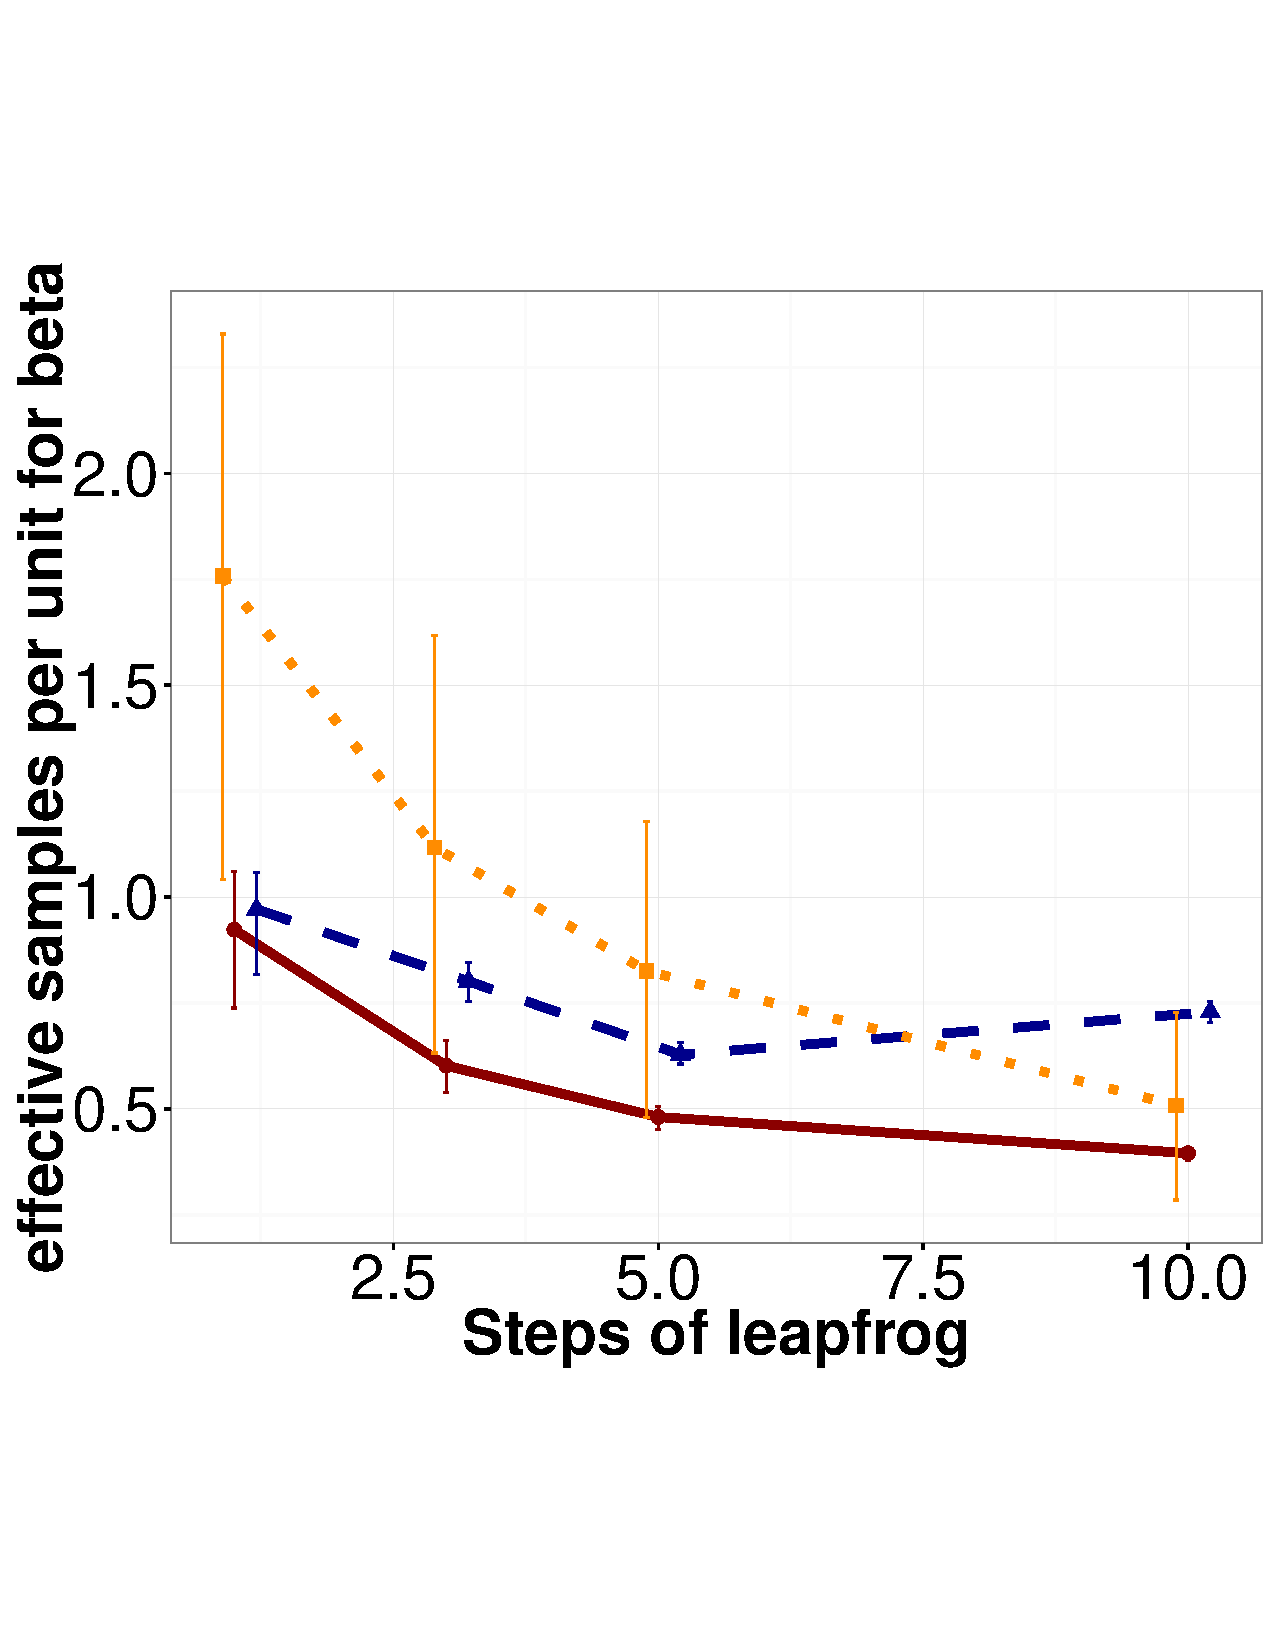
\includegraphics [width=0.70\textwidth, angle=0]{figs/h_beta.pdf}
      \end{minipage}

    \caption{HMC for dim 3}
  \end{figure}


  \begin{figure}%[b]
  \centering
  \begin{minipage}[hp]{0.45\linewidth}
  \centering
    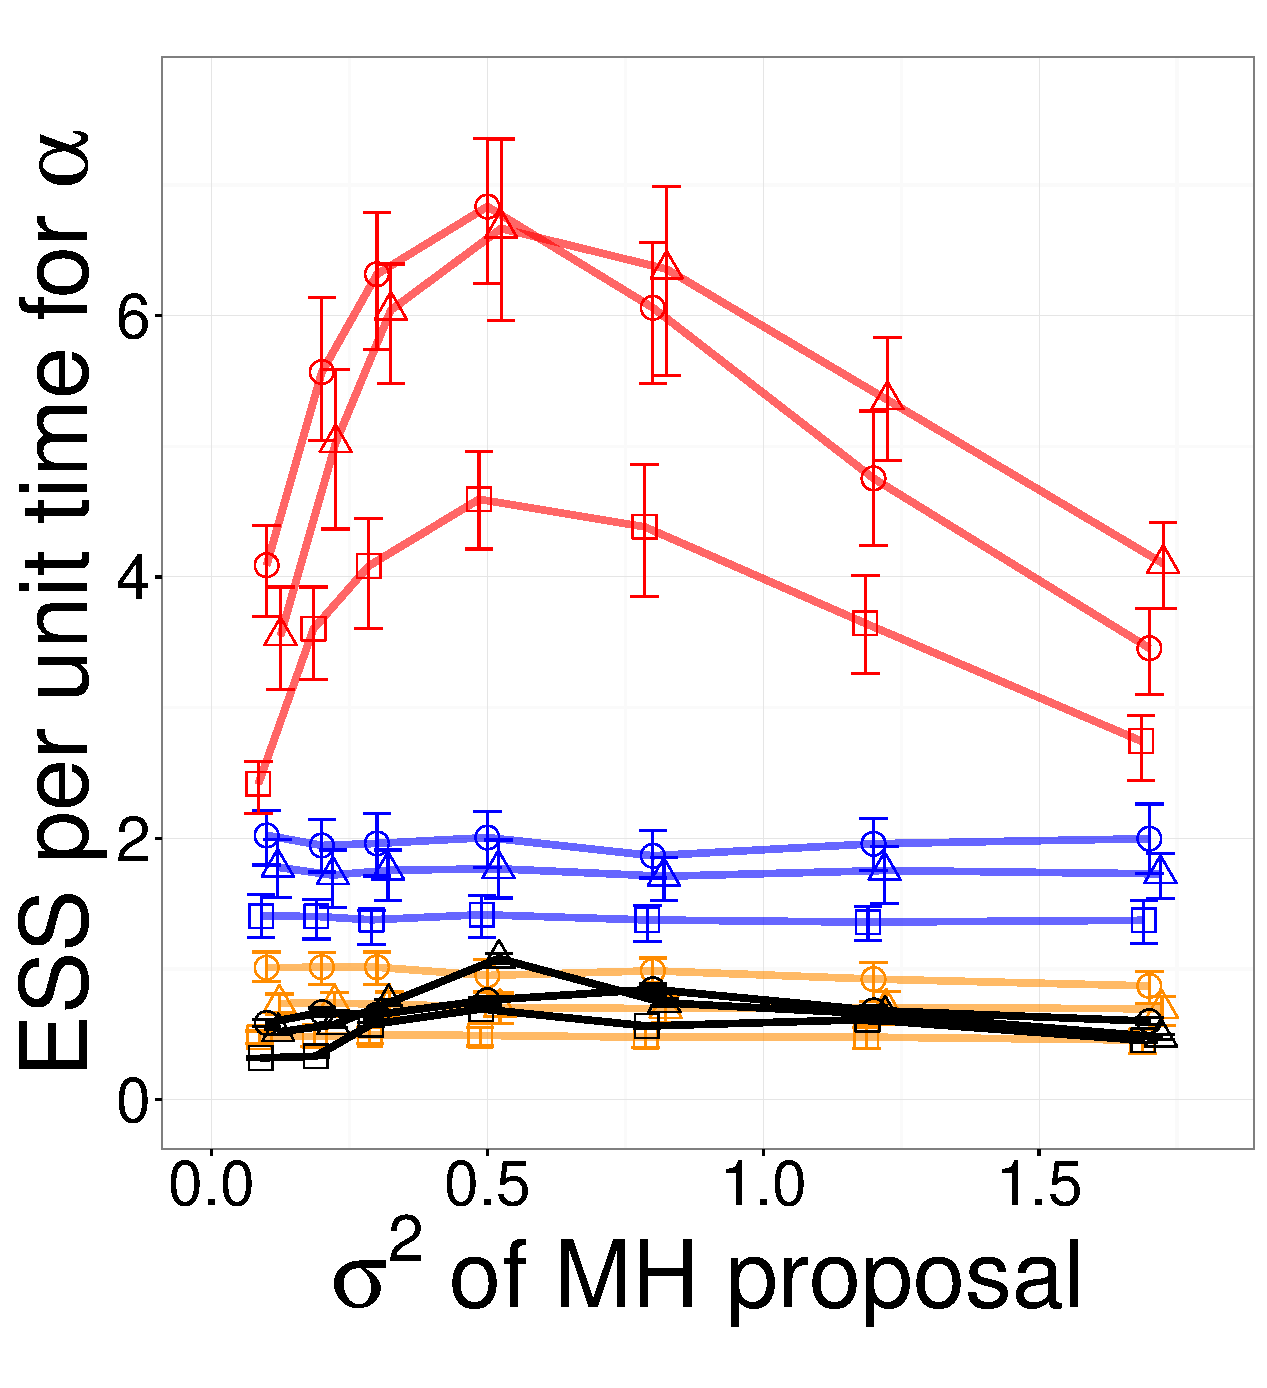
\includegraphics [width=0.70\textwidth, angle=0]{figs/exp_5_alpha.pdf}
%    \caption{ESS/sec for exp model (alpha, dim 5)}
      \end{minipage}
  \begin{minipage}[hp]{0.45\linewidth}
  \centering
    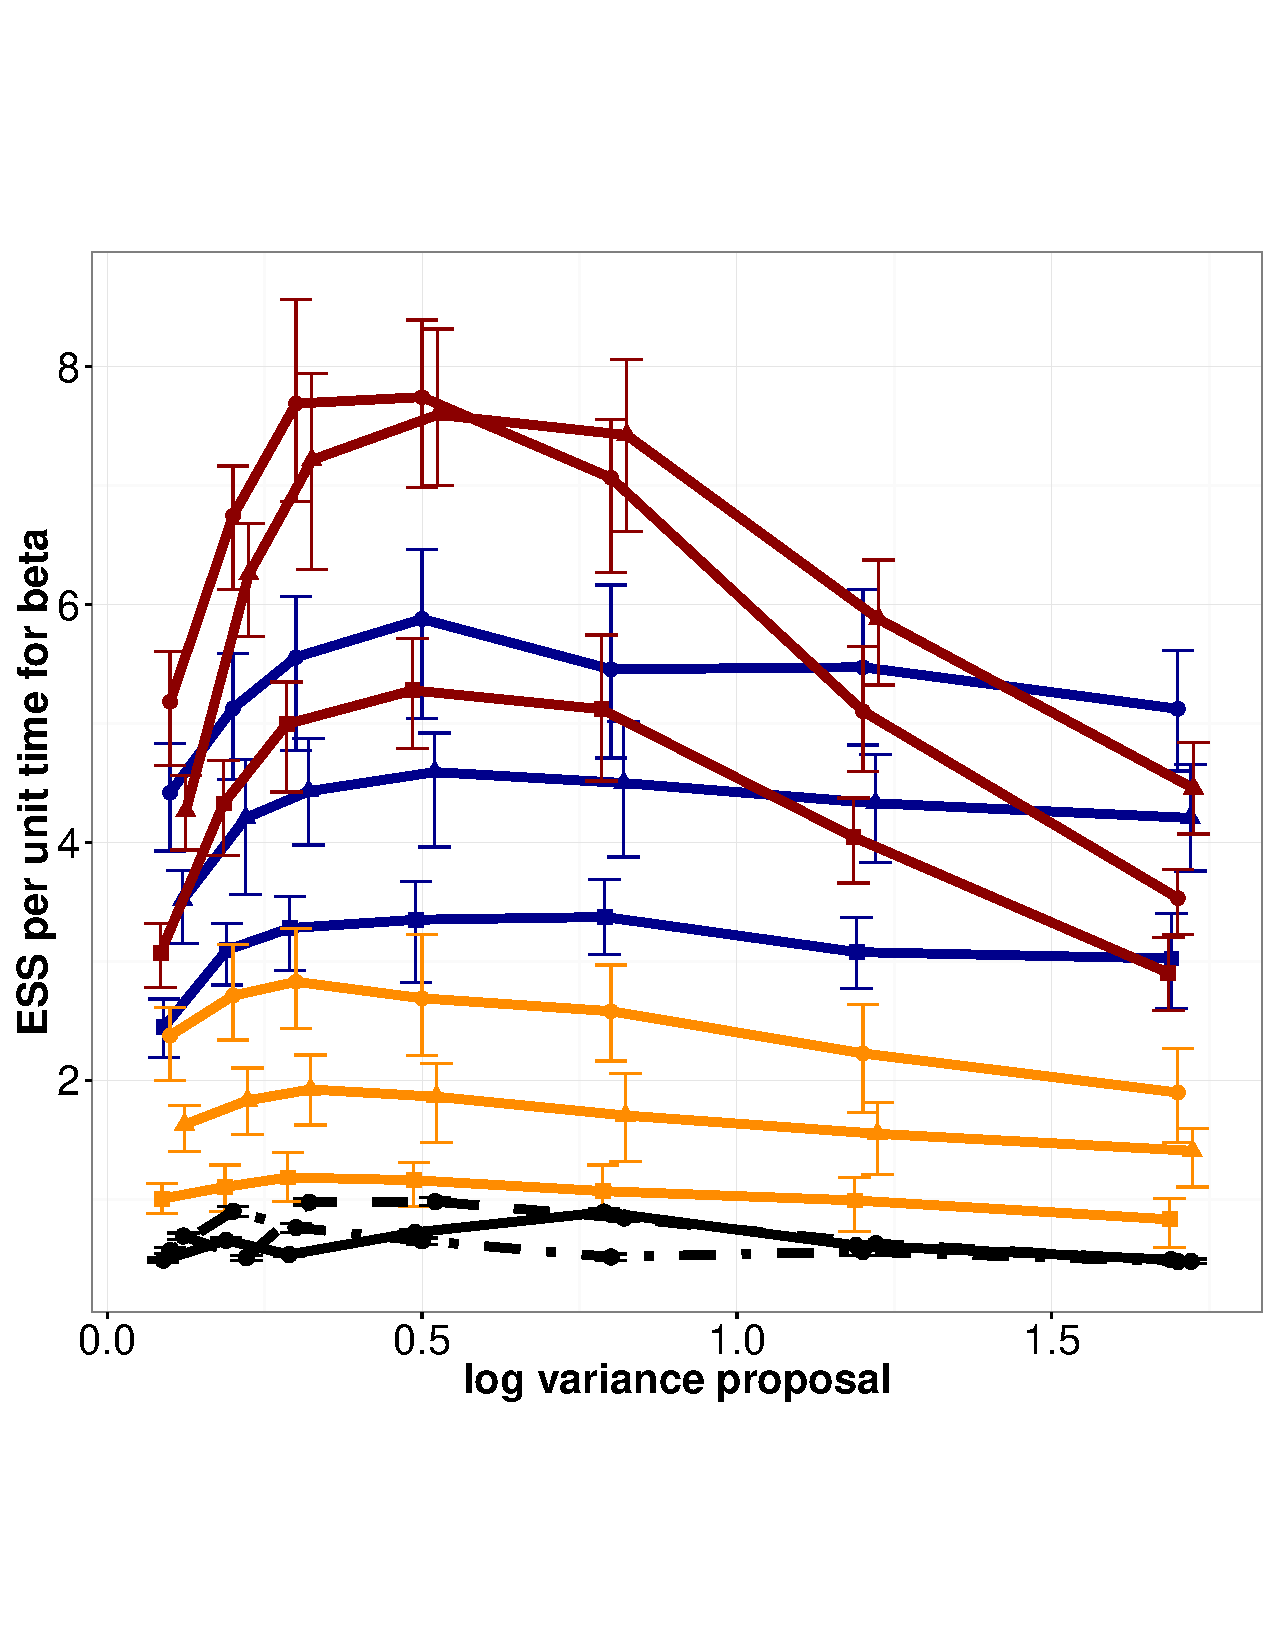
\includegraphics [width=0.70\textwidth, angle=0]{figs/exp_5_beta.pdf}
    \vspace{-0 in}
%    \caption{ESS/sec for exp model (beta, dim 5)}
     \label{fig:ESS_EXP_D5}
  \end{minipage}
    \caption{ESS/sec for exp model (dim 5)}
  \end{figure}

  \begin{figure}%[b]
  \centering
  \begin{minipage}[hp]{0.45\linewidth}
  \centering
    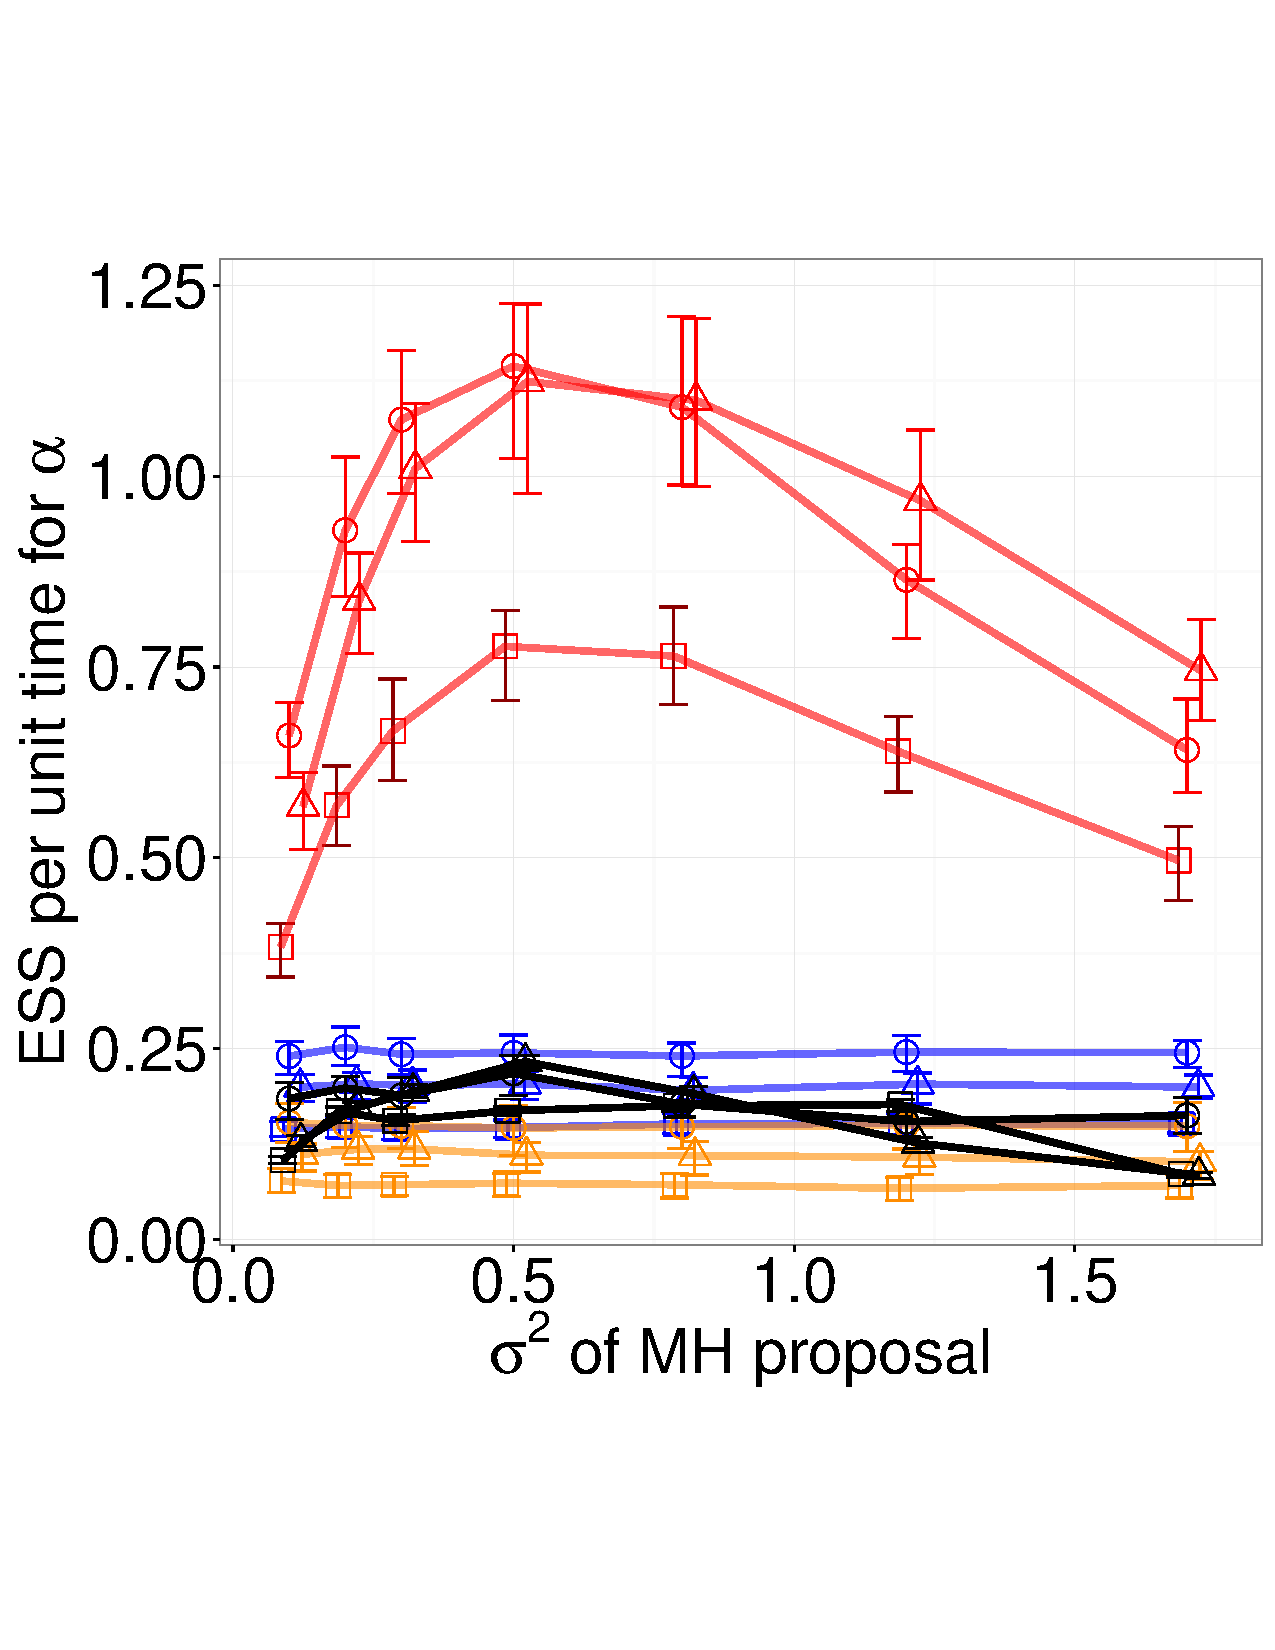
\includegraphics [width=0.70\textwidth, angle=0]{figs/exp_10_alpha.pdf}
      \end{minipage}
  \begin{minipage}[!hp]{0.45\linewidth}
  \centering
    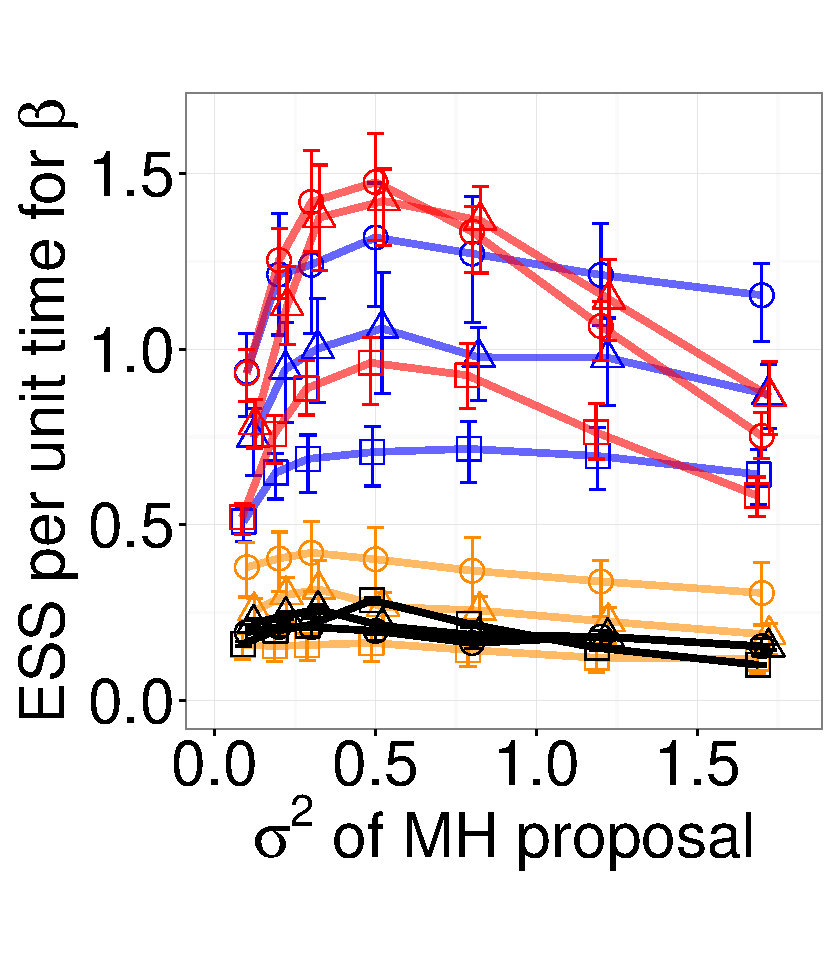
\includegraphics [width=0.70\textwidth, angle=0]{figs/exp_10_beta.pdf}
    \vspace{-0 in}
     \label{fig:ESS_EXP_D10}
  \end{minipage}
    \caption{ESS/sec for exp model (dim 10)}
  \end{figure}
  
  
  
  \begin{figure}%[b]
  \centering
  \begin{minipage}[hp]{0.45\linewidth}
  \centering
    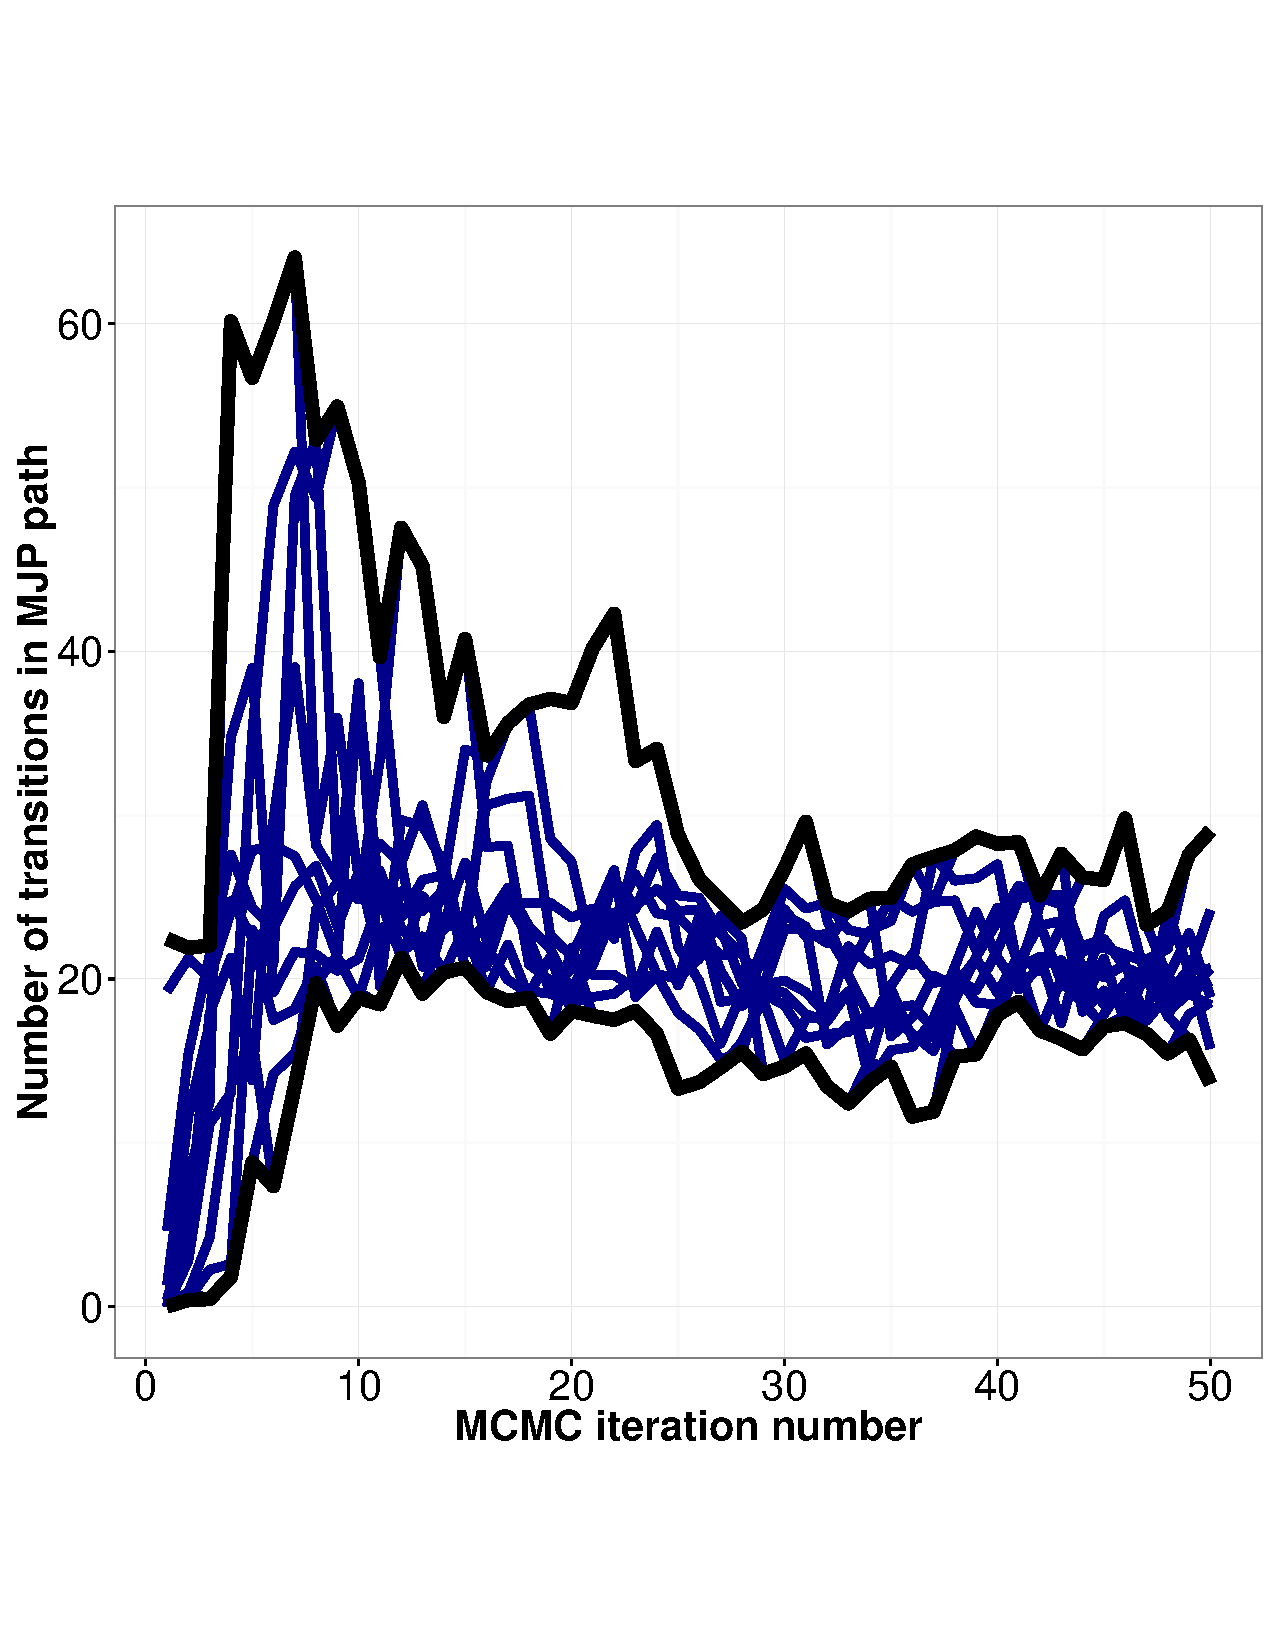
\includegraphics [width=0.70\textwidth, angle=0]{figs/exp3_k2_path_transition.pdf}
    \caption{Trace plot of the number of MJP transitions for different initializatoins for exponential model.}
      \end{minipage}
  \end{figure}

  \begin{figure}%[b]
  \centering
  \begin{minipage}[hp]{0.45\linewidth}
  \centering
    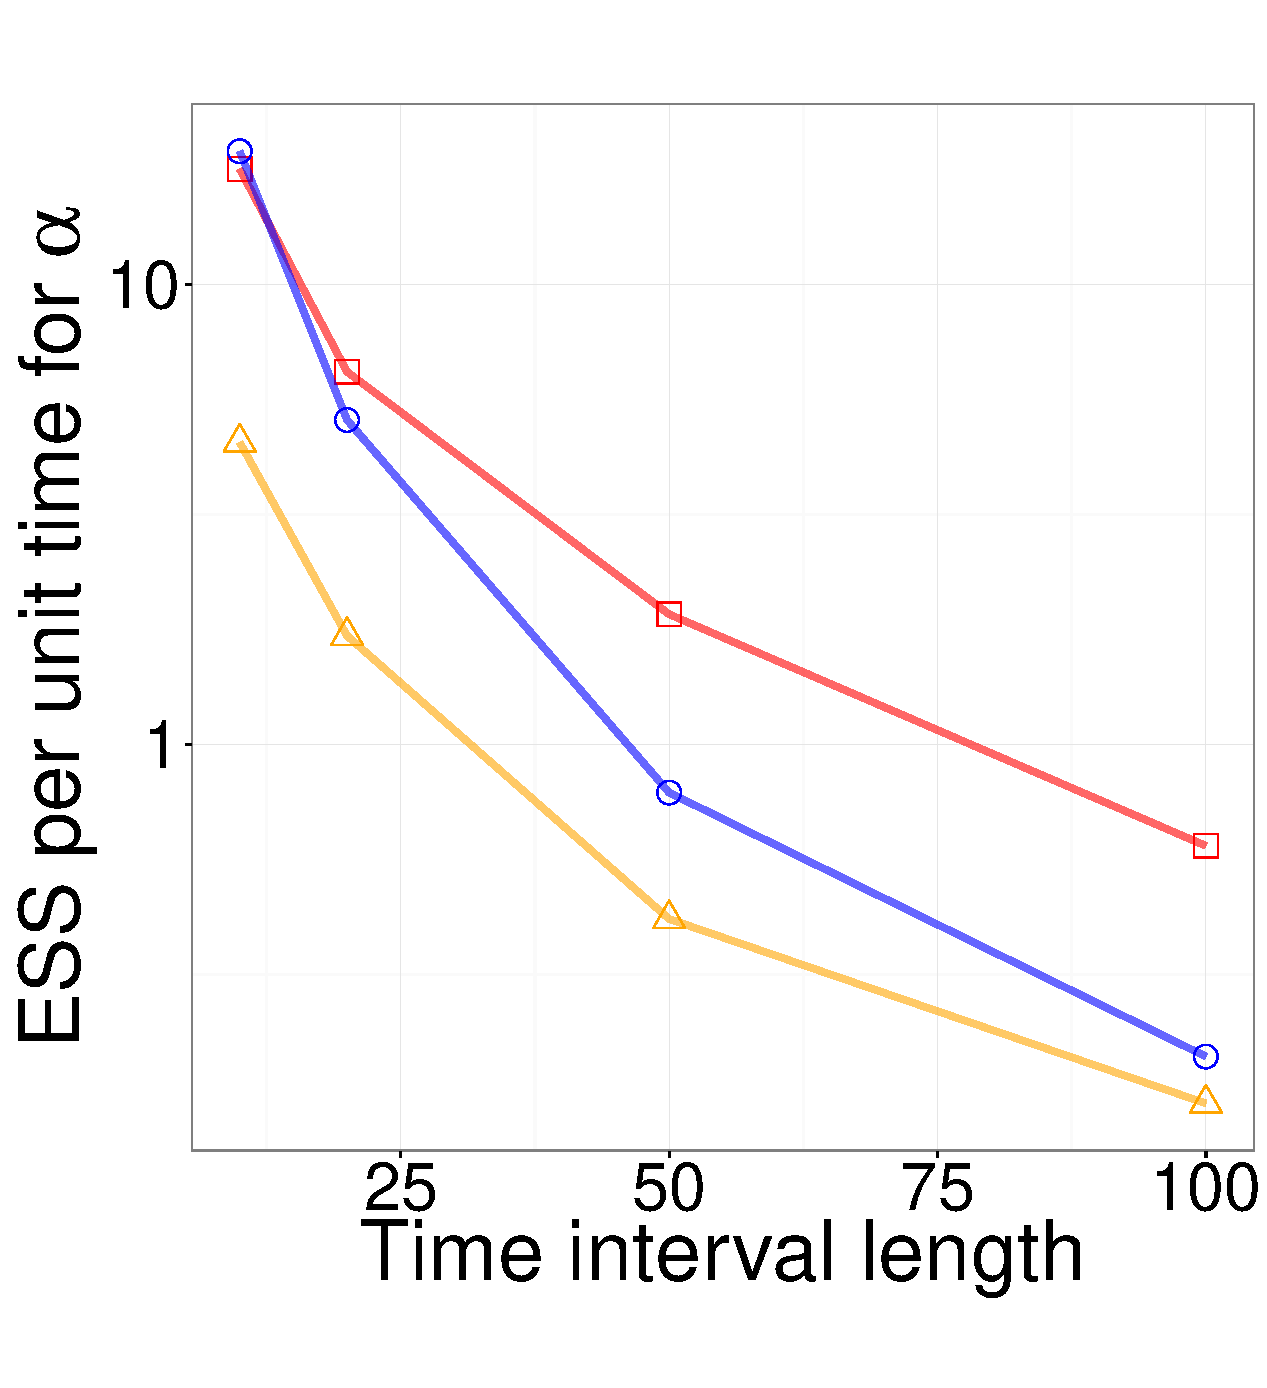
\includegraphics [width=0.70\textwidth, angle=0]{figs/ESS_vs_t_alpha.pdf}
      \end{minipage}
  \begin{minipage}[hp]{0.45\linewidth}
  \centering
    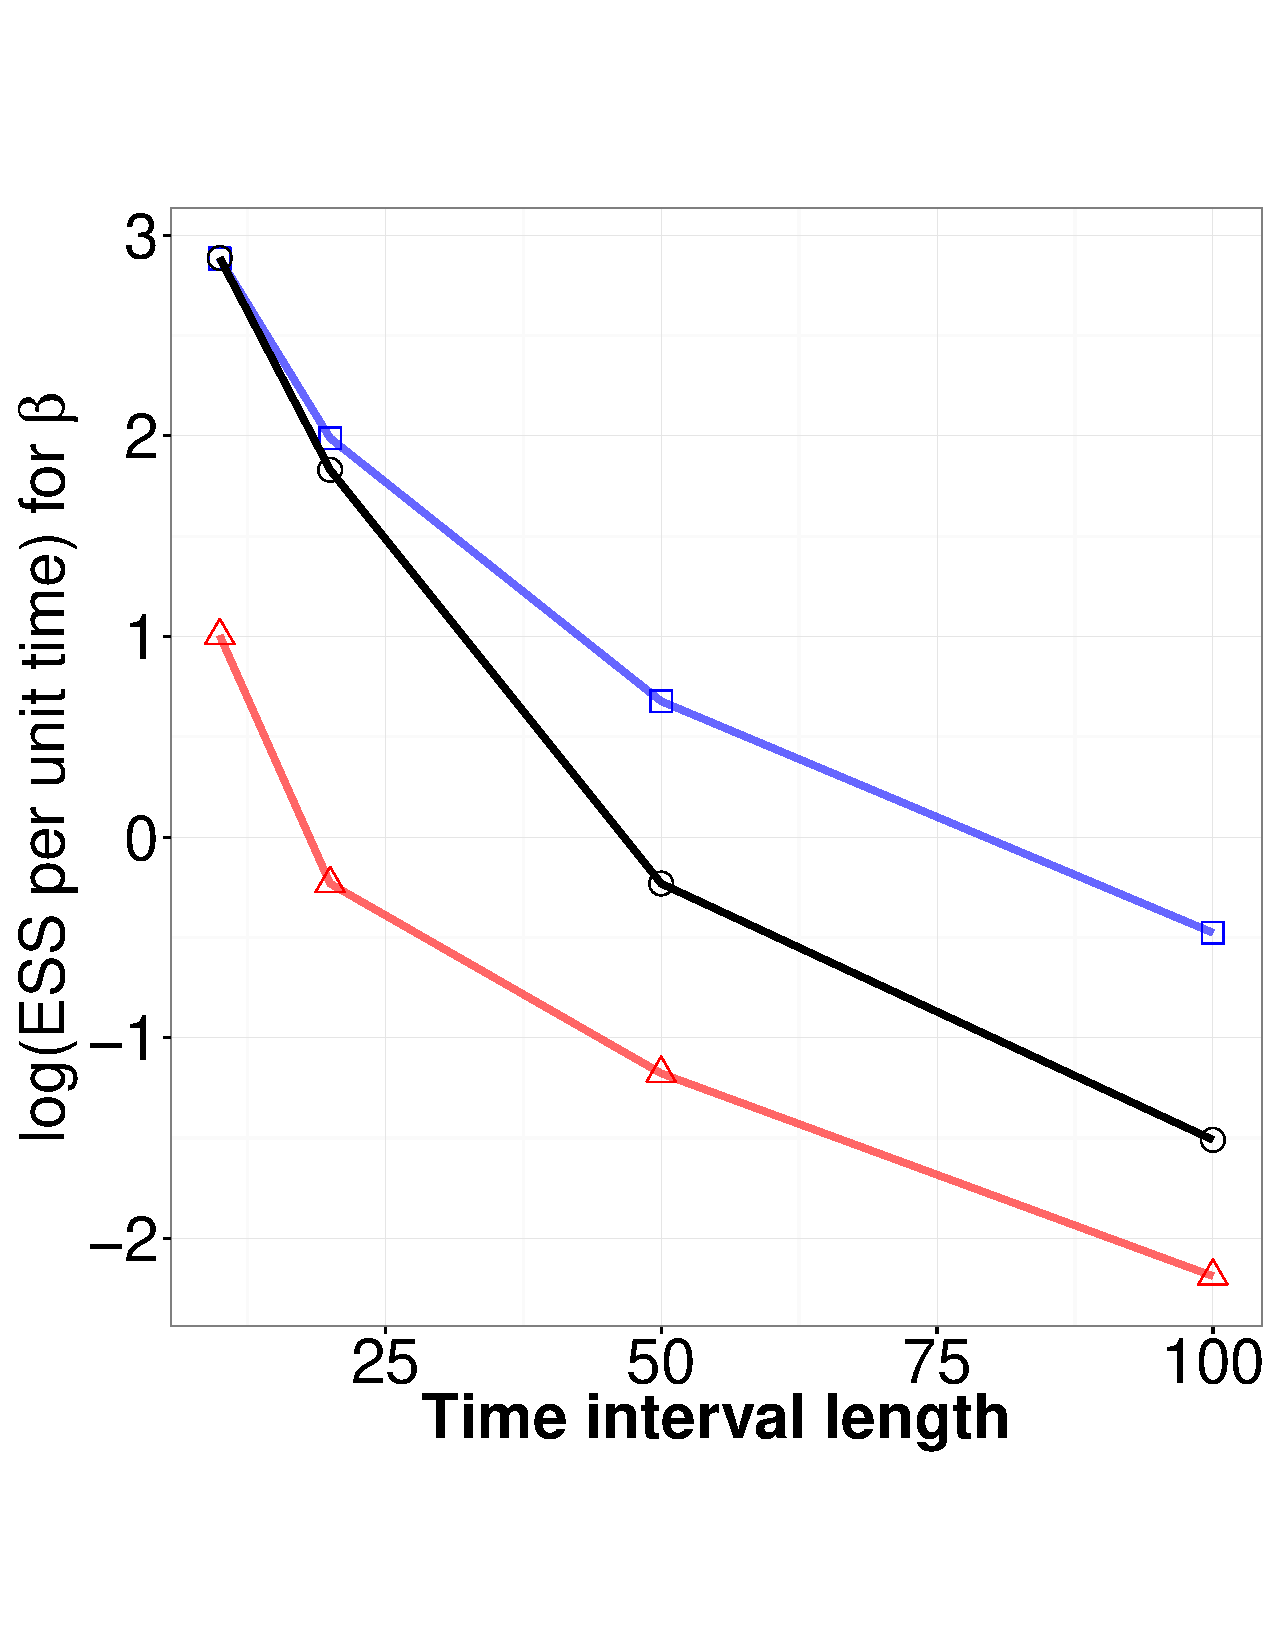
\includegraphics [width=0.70\textwidth, angle=0]{figs/ESS_vs_t_beta.pdf}
    \vspace{-0 in}
     \label{fig:TSS}
  \end{minipage}
    \caption{Time Interval vs. ESS / sec}
  \end{figure}

  \begin{figure}%[b]  
  \centering
  \begin{minipage}[hp]{0.45\linewidth}
  \centering
    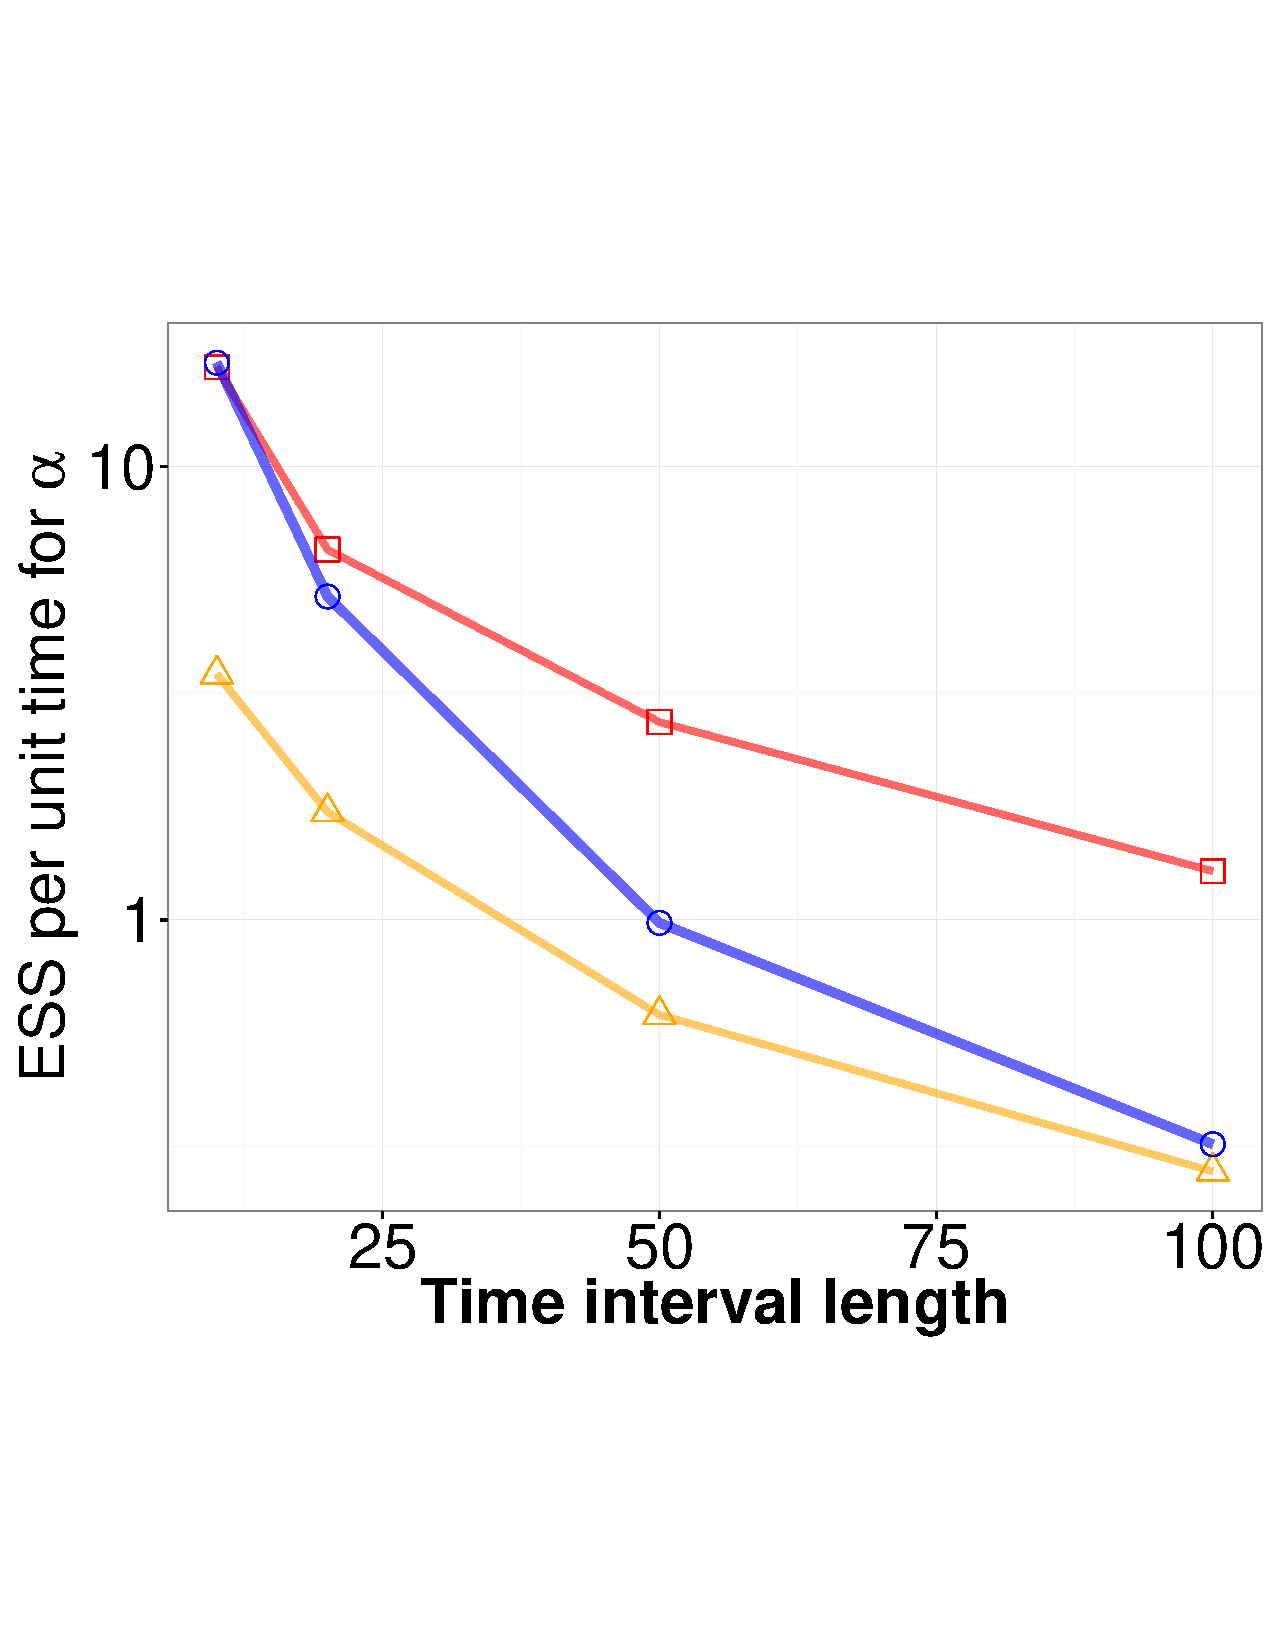
\includegraphics [width=0.70\textwidth, angle=0]{figs/ESS_vs_t_alpha_fixobservation.pdf}
    \end{minipage}
  \begin{minipage}[hp]{0.45\linewidth}
  \centering
    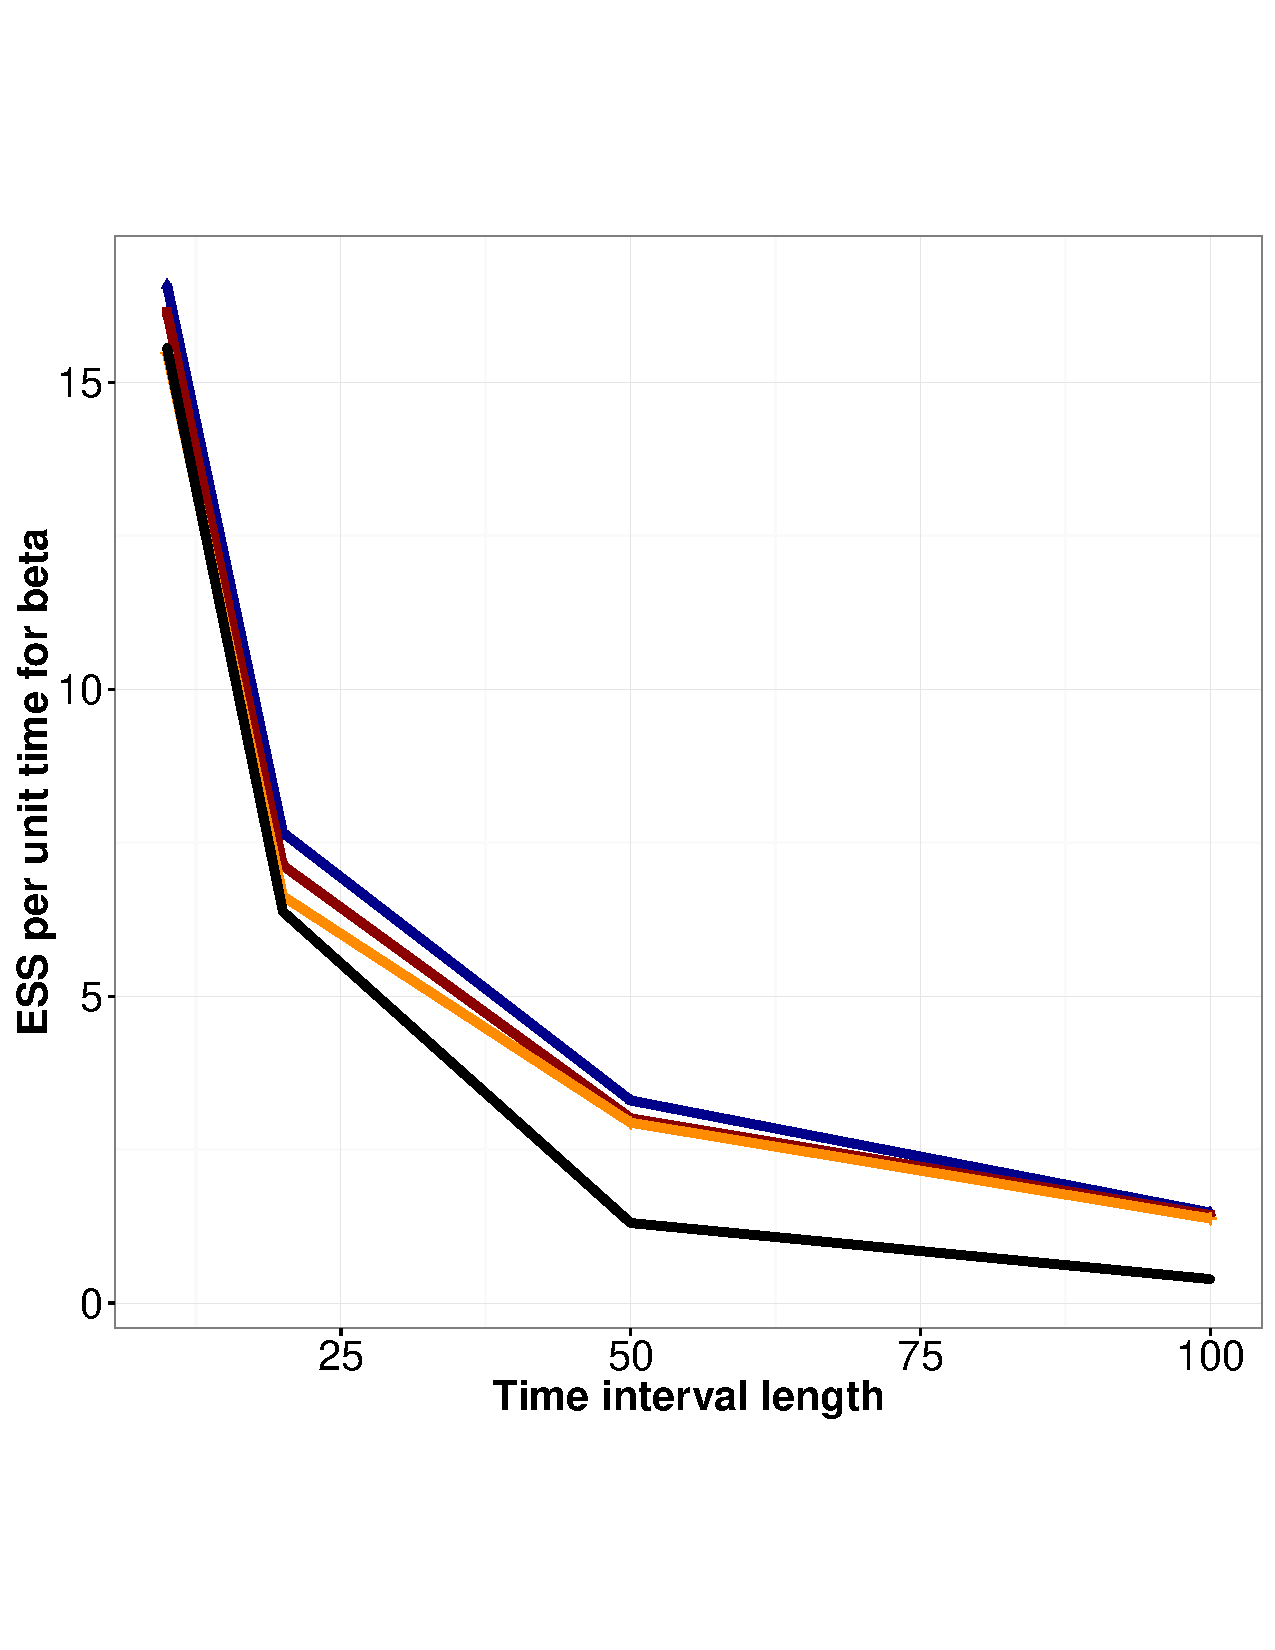
\includegraphics [width=0.70\textwidth, angle=0]{figs/ESS_vs_t_beta_fixobservation.pdf}
    \vspace{-0 in}
     \label{fig:TSS}
  \end{minipage}
    \caption{Time Interval vs. ESS / sec (Number of observations is fixed)}
  \end{figure}
  \begin{figure}%[b]
  \centering
  \begin{minipage}[hp]{0.45\linewidth}
  \centering
    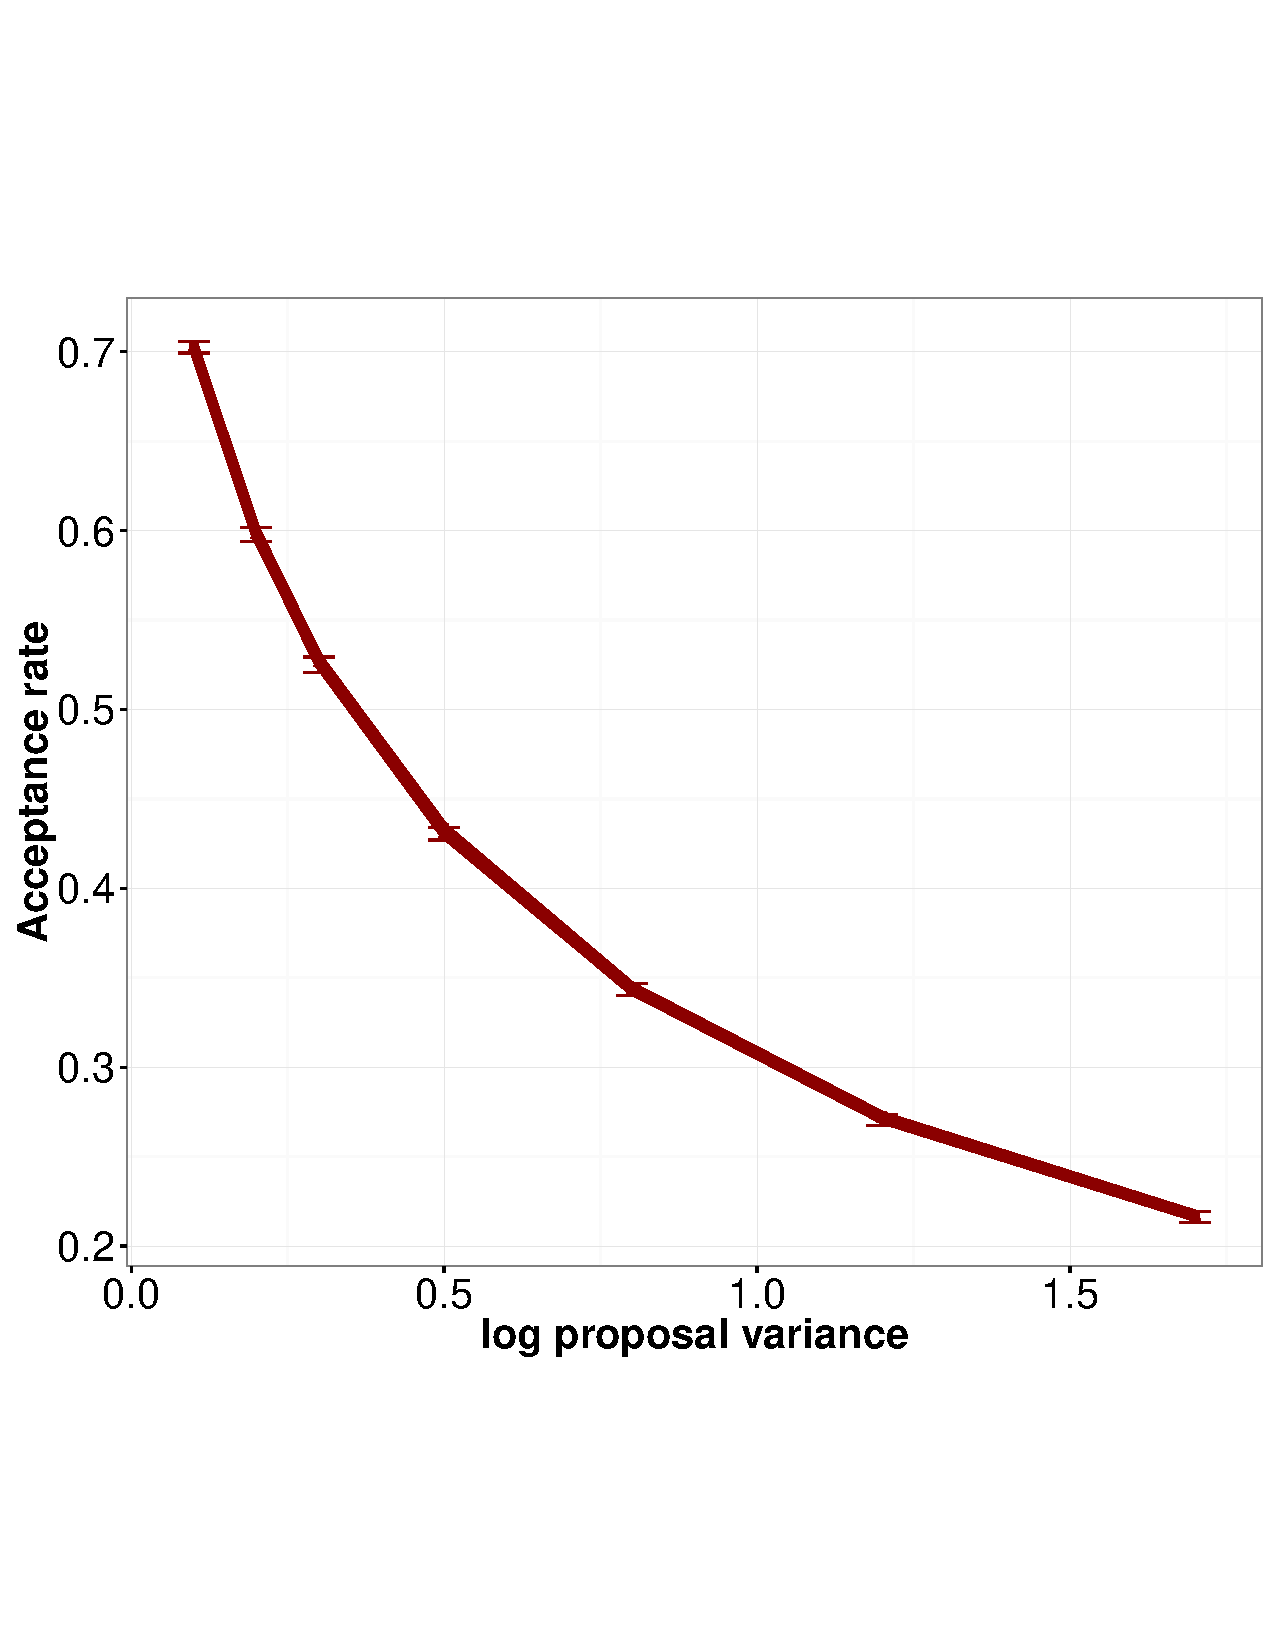
\includegraphics [width=0.70\textwidth, angle=0]{figs/acc_rate_exp_d3.pdf}
    \caption{Acceptance rate for exp model (dim 3)}
      \end{minipage}
  \end{figure}


\section{Immigration models with capacity}~
An $M/M/N/N$ queue is a stochastic process whose state space is the set $\{0, 1, 2, 3, ..., N - 1\}$ where the value corresponds to the number of customers in the system, including any currently in service. Arrivals occur at rate $\alpha$ according to a Poisson process and move the process from state $i$ to $i+1$. Service times have an exponential distribution with parameter $\beta$ in the $M/M/N/N$ queue. There are $N$ servers, which serve from the front of the queue. If there are less than $N$ jobs, some of the servers will be idle. Only $N$ customers can queue at any one time. Any further arrivals to the queue are considered "lost". 
  \begin{figure}[H]
  \centering
  \begin{minipage}[!hp]{0.6\linewidth}%0.45
  \centering
    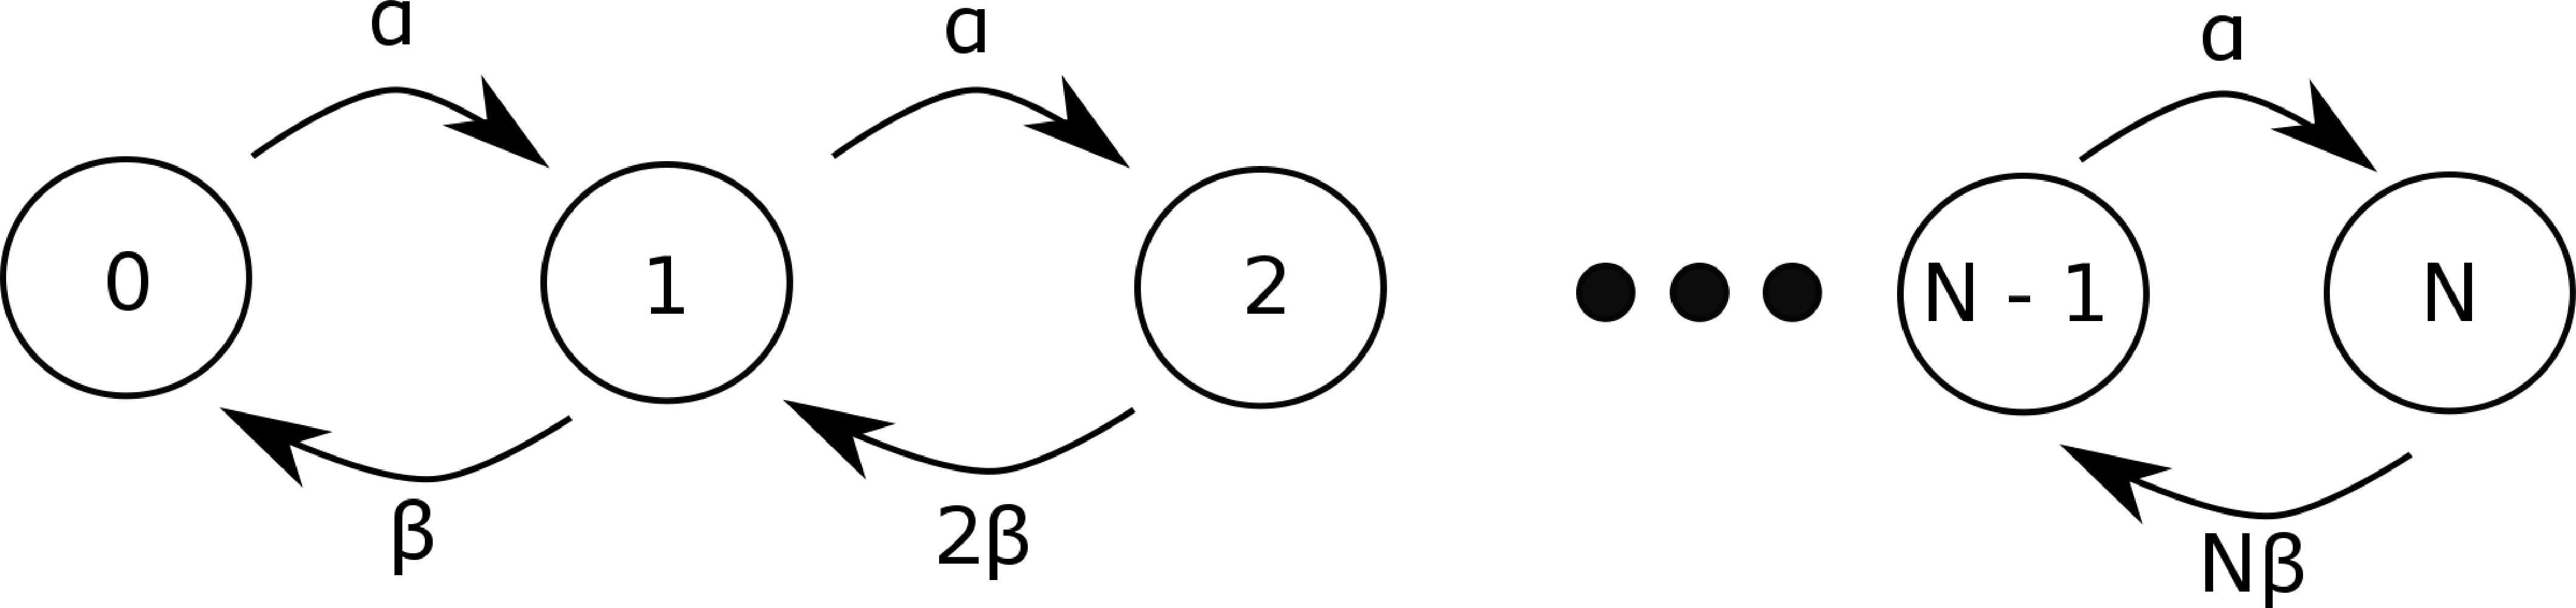
\includegraphics [width=1\textwidth, angle=0]{figs/qplot2.png}%0.70
      \end{minipage}
    \caption{exp model}
  \end{figure}

\noindent Assume: $S = [S_0,S_1, ...,S_N] \;, T = [t_0(t_{start}), t_1,...,t_N, t_{N+1}(t_{end})]$, and y as observations.\\
Now, let's consider a immigration model as follows. State space is $\{0, 1, 2, ..., N - 1\}$, representing the total population. The transition matrix is defined as follows. 
$$A_i =: A_{i,i} = -(\alpha + i\beta), \; \; i =0,1,...,N$$ $$A_{i, i+1} = \alpha, \; \; i =0,1,...,N-1,$$ $$A_{i, i-1}  = \beta, \; \;  i =1,...,N.$$
We already know the conditional density(given $\alpha,\; \beta$) of a MJP trajectory $(s_0, S, T)$ in time interval $[t_{start}, t_{end}]$, with $S=(s_1, s_2,..., s_k)$, $T=(t_1, t_2,..., t_k)$. 
$$f(s_0,S,T| \alpha, \beta) = \prod_{i=0}^{k-1} A_{s_i, s_{i+1}} \exp(\sum_{i=0}^{k} A_{s_i}(t_{i+1} - t_{i})), $$
where $t_0 = t_{start}$, $t_{k+1} = t_{end}.$\\
Let's denote some notations here.\\
$$U(s_0, S, T):= \sum_{i=0}^{k-1} \mathbb{I}_{\{s_{i+1} - s_i = 1\}}.$$
$$D(s_0, S, T):= \sum_{i=0}^{k-1} \mathbb{I}_{\{s_{i+1} - s_i = -1\}}.$$
Call them U and D for short.
Let's denote the total time when the trajectory state stays at state i as $\tau_i$, i.e. $\tau_i = \sum_{j=0}^{k} (t_{j+1} -t_j)\mathbb{I}_{\{s_j = i\}}$, then $\sum_{i=0}^k (t_{i+1} - t_i)s_i = \sum_{i=0}^N \tau_ii.$\\

$$f(s_0,S,T| \alpha, \beta) = \exp(-\alpha(t_{end} - t_{start}- \tau_N) )\alpha^U \cdot  \exp((-(\sum_{i=0}^k (t_{i+1} - t_i)s_i)\beta) \prod_{i=1}^N i^{\sum_{j=0}^{k-1}\mathbb{I}_{s_{j+1} = i -1 \;,  s_j = i} }   \beta^D$$\\
If we assume the prior of $\alpha$, and $\beta$ are $Gamma(\mu,\lambda)$, $Gamma(\omega, \theta)$, which are independent with each other. \\
$$p(\alpha) = \frac{\lambda^\mu}{\Gamma(\mu)}\alpha^{\mu -1}e^{-\lambda \alpha}. $$
$$p(\beta) = \frac{\theta^\omega}{\Gamma(\omega)}\beta^{\omega -1}e^{-\theta \beta}. $$
Then we can get the posterior distribution $$f(\alpha, \beta | s_0,S,T)$$ as follows.
$$ f(\alpha, \beta | s_0,S,T) \propto \exp(-(\lambda + t_{end} - t_{start}- \tau_N)\alpha) \alpha^{\mu + U -1} \cdot \exp(-(\sum_{i=0}^k (t_{i+1} - t_i)s_i + \theta)\beta) \beta^{\omega+ D -1}.$$
It means that the posterior distributions of $\alpha$, $\beta$ are still independent. \\
$\alpha | s_0,S,T$ is following $Gamma(\mu+ U,\lambda + t_{end} - t_{start}- \tau_N)$\\
$\beta | s_0,S,T$ is following $Gamma(\omega+ D,\theta + \sum_{i=0}^k (t_{i+1} - t_i)s_i)$, which is equivalent to $Gamma(\omega+ D,\theta +\sum_{i=0}^N \tau_ii)$\\
Such immigration models have perfectly conjugate posterior distributions when we assign $\gamma$ priors to $\alpha$ and $\beta$. We apply our Metropolis Hasting algorithms on such models to compare the performance with the performance of Gibbs Sampling algorithm.
\subsection{Experiments}
In the following, we evaluate a Python implementation of our algorithms compared to other exact samplers which include Gibbs sampler and Particle MCMC sampler. We consider three different dimensions which are 3, 5, and 10 and three different k which are 1.5, 2, and 3. We generated random parameters $\alpha$, $\beta$ from prior distributions ($Gamma(3,2), Gamma(5, 2)$), and used this to construct the transition matrix A. Then we generate an MJP trajectory with a uniform initial distribution over states. The state of this MJP trajectory was observed via a Normal distribution with mean equal to the value of state and variance 1, and posterior samples given the observations were produced by a Python implementation of our algorithm. 100 MCMC runs were performed, each run consisting of 10000(Varies among different dimensions) iterations. For each run, the number of transitions as well as the time spent was calculated, and effective sample sizes (ESSs) of these statistics (the number of independent samples with the same `information' as the correlated MCMC samples) were calculated using R-CODA (Plummer et al., 2006). The overall ESS of a run is defined to be the mean ESS across all these ESSs.

  \begin{figure}%[b]
  \centering
  \begin{minipage}[!hp]{0.45\linewidth}
  \centering
    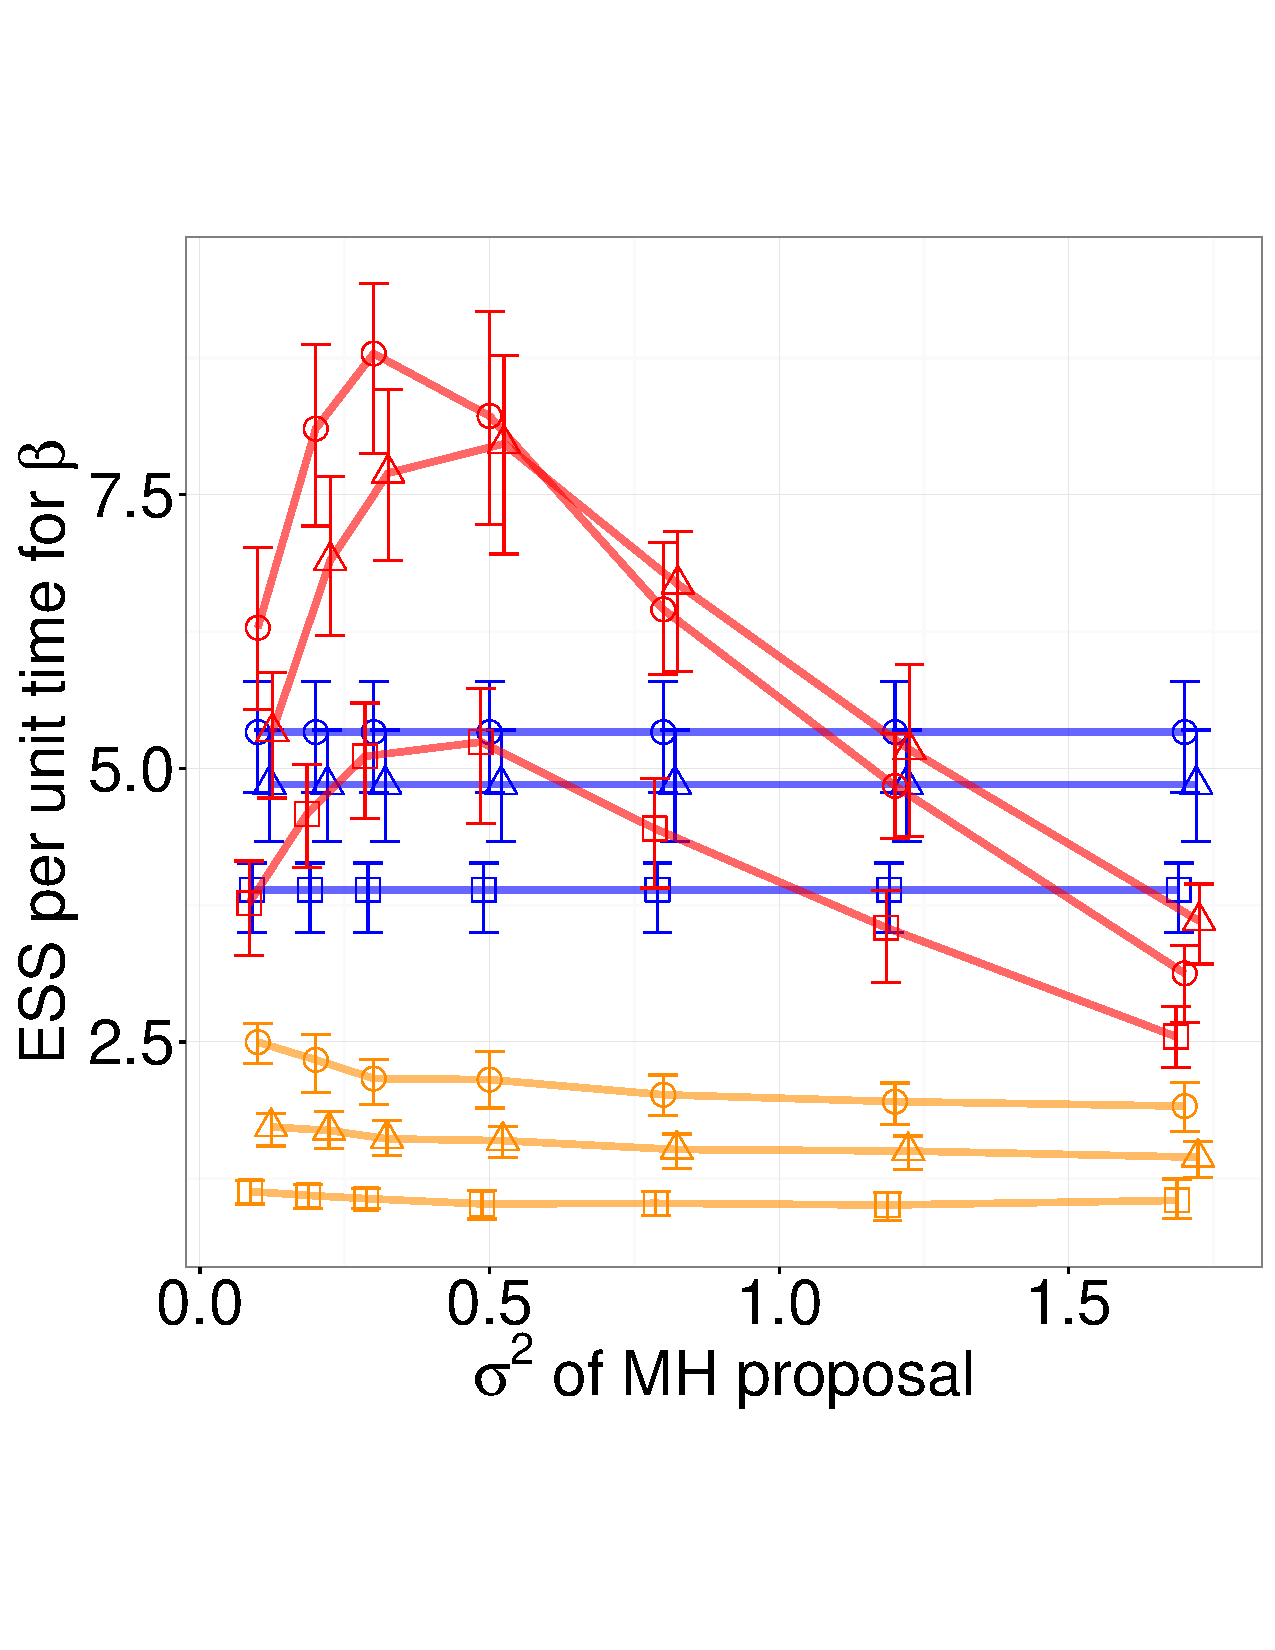
\includegraphics [width=0.70\textwidth, angle=0]{figs/q_3_alpha.pdf}
      \end{minipage}
  \begin{minipage}[!hp]{0.45\linewidth}
  \centering
    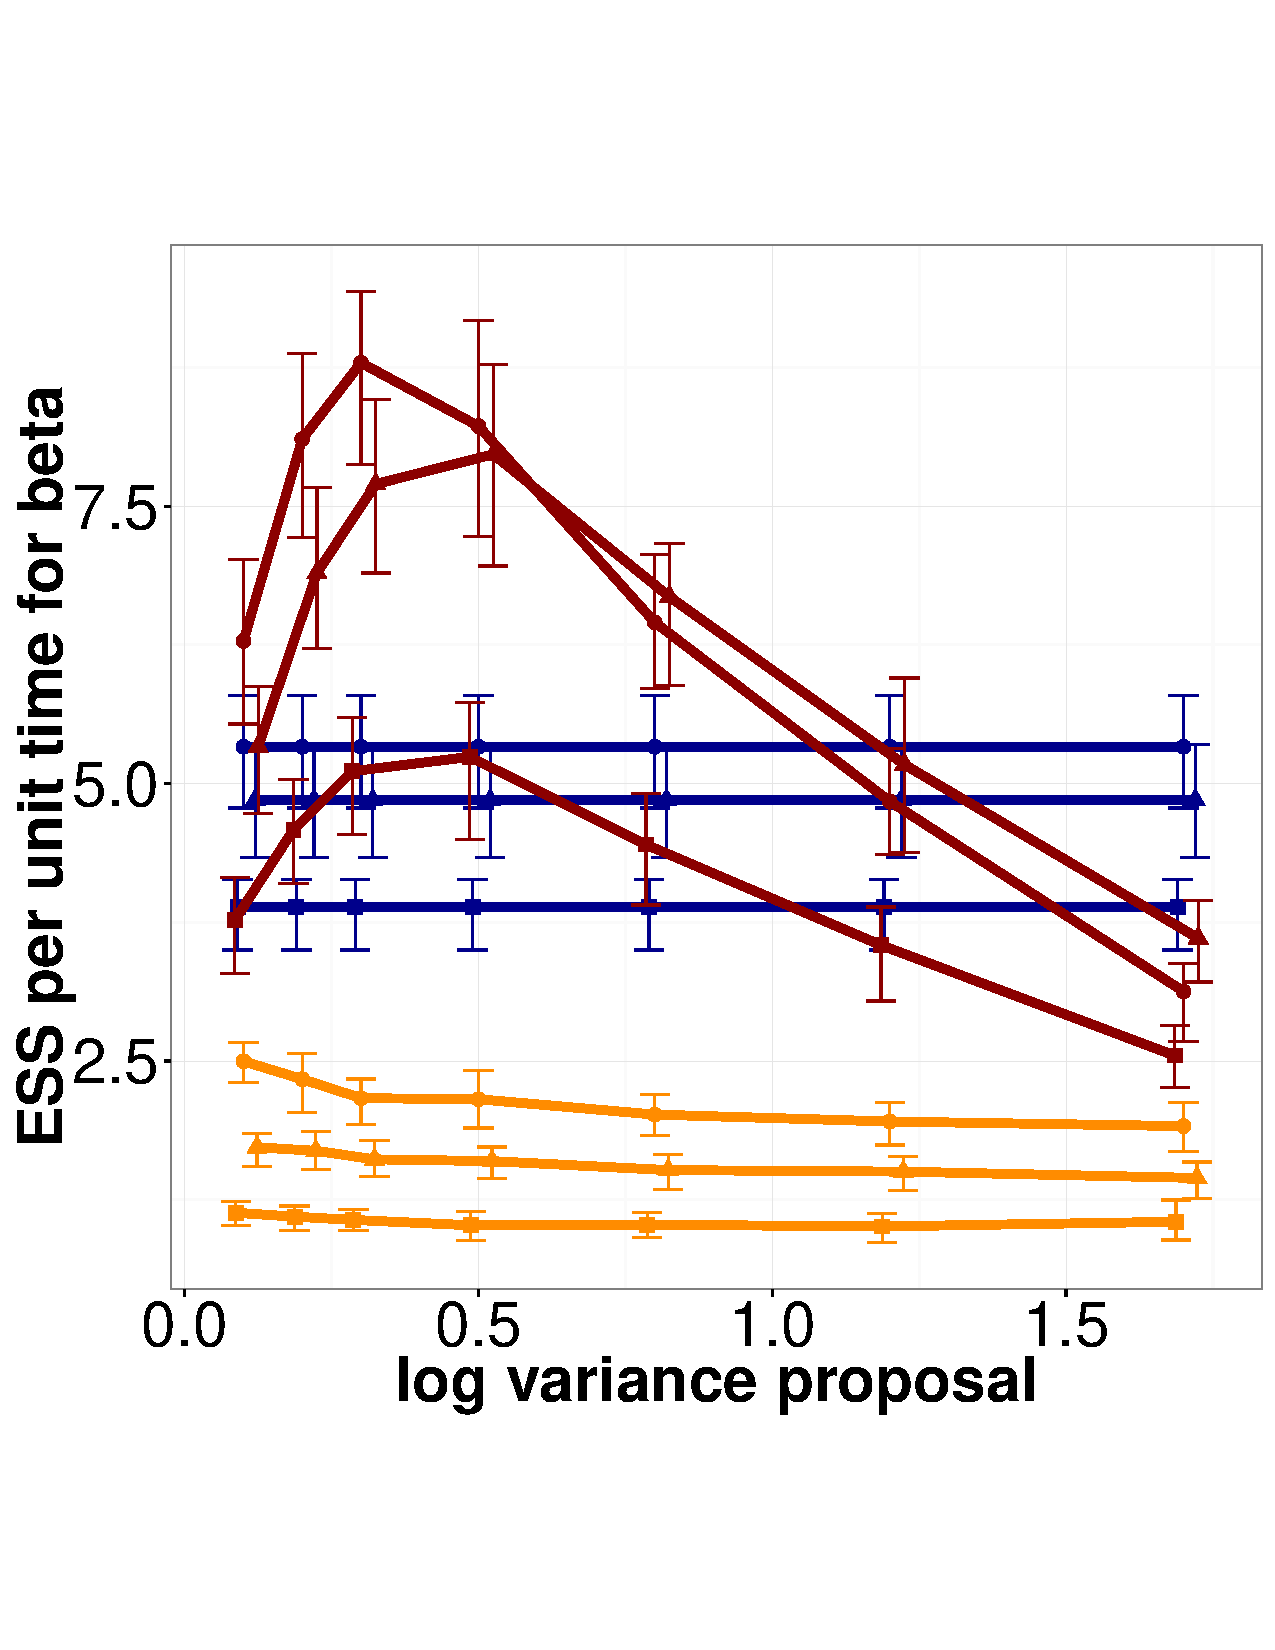
\includegraphics [width=0.70\textwidth, angle=0]{figs/q_3_beta.pdf}
    \vspace{-0 in}
     \label{fig:ESS_Q_3}
  \end{minipage}
    \caption{ESS/sec for Immigration model (dim 3)}
  \end{figure}
  \begin{figure}%[b]
  \centering
  \begin{minipage}[!hp]{0.45\linewidth}
  \centering
    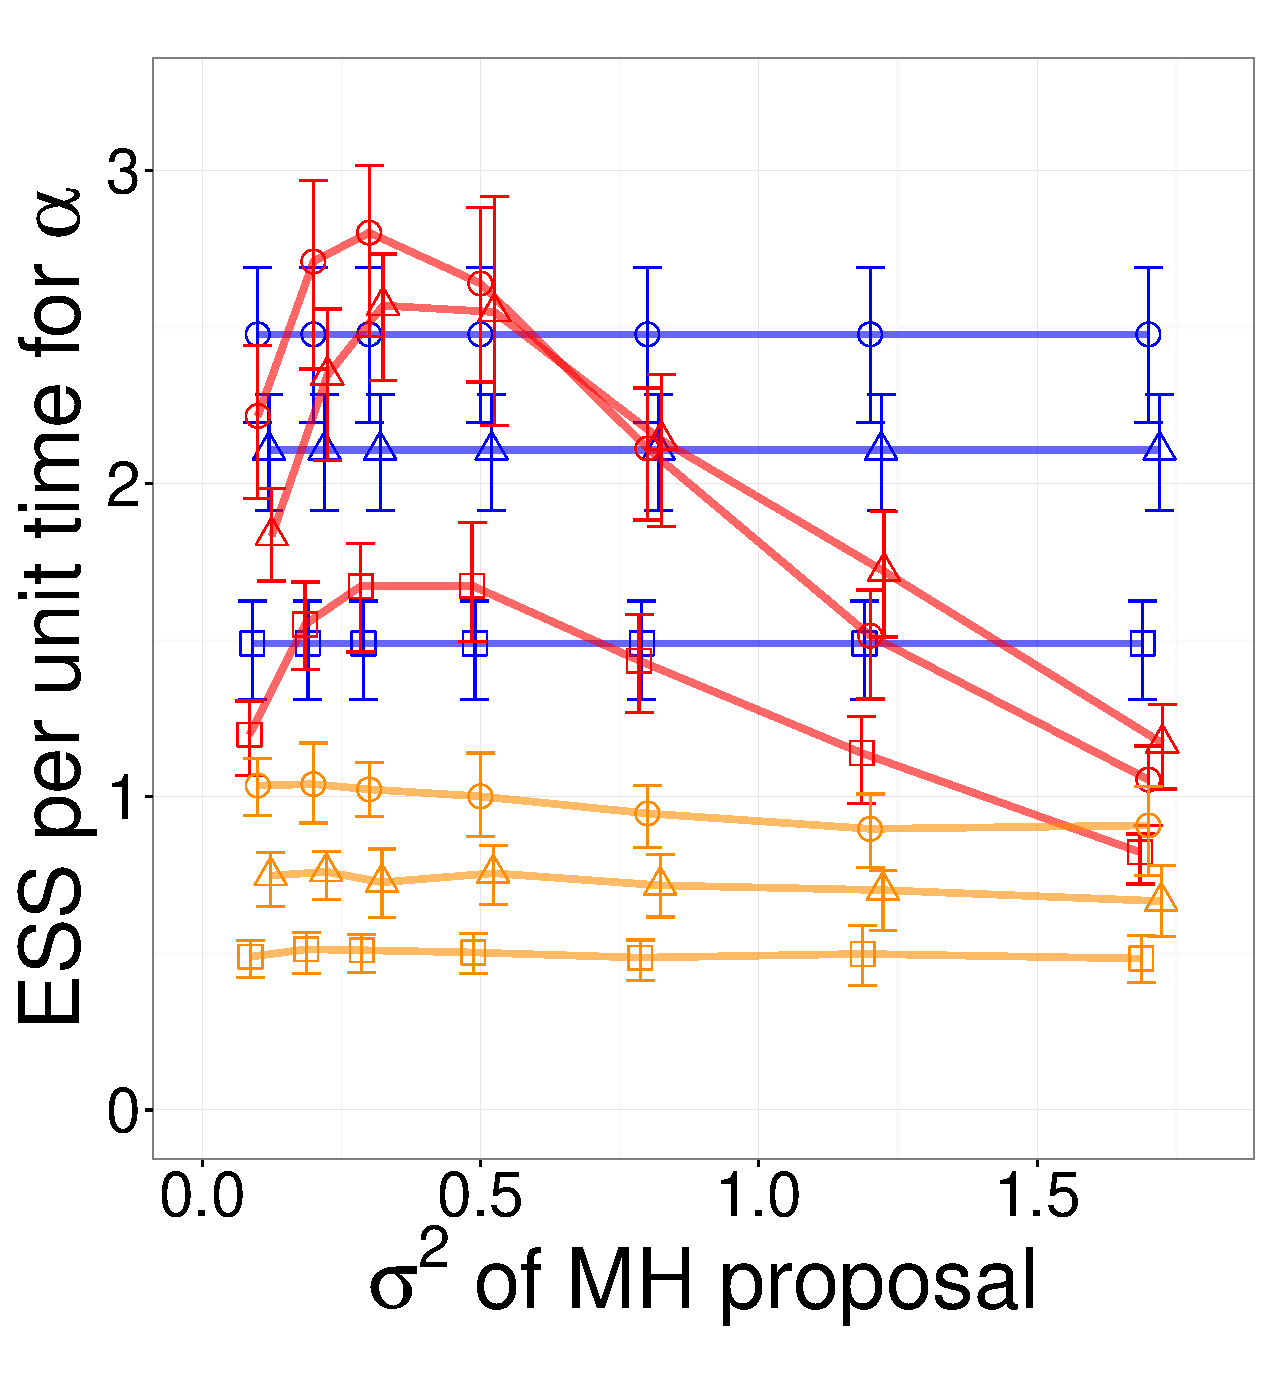
\includegraphics [width=0.70\textwidth, angle=0]{figs/q_5_alpha.pdf}
      \end{minipage}
  \begin{minipage}[!hp]{0.45\linewidth}
  \centering
    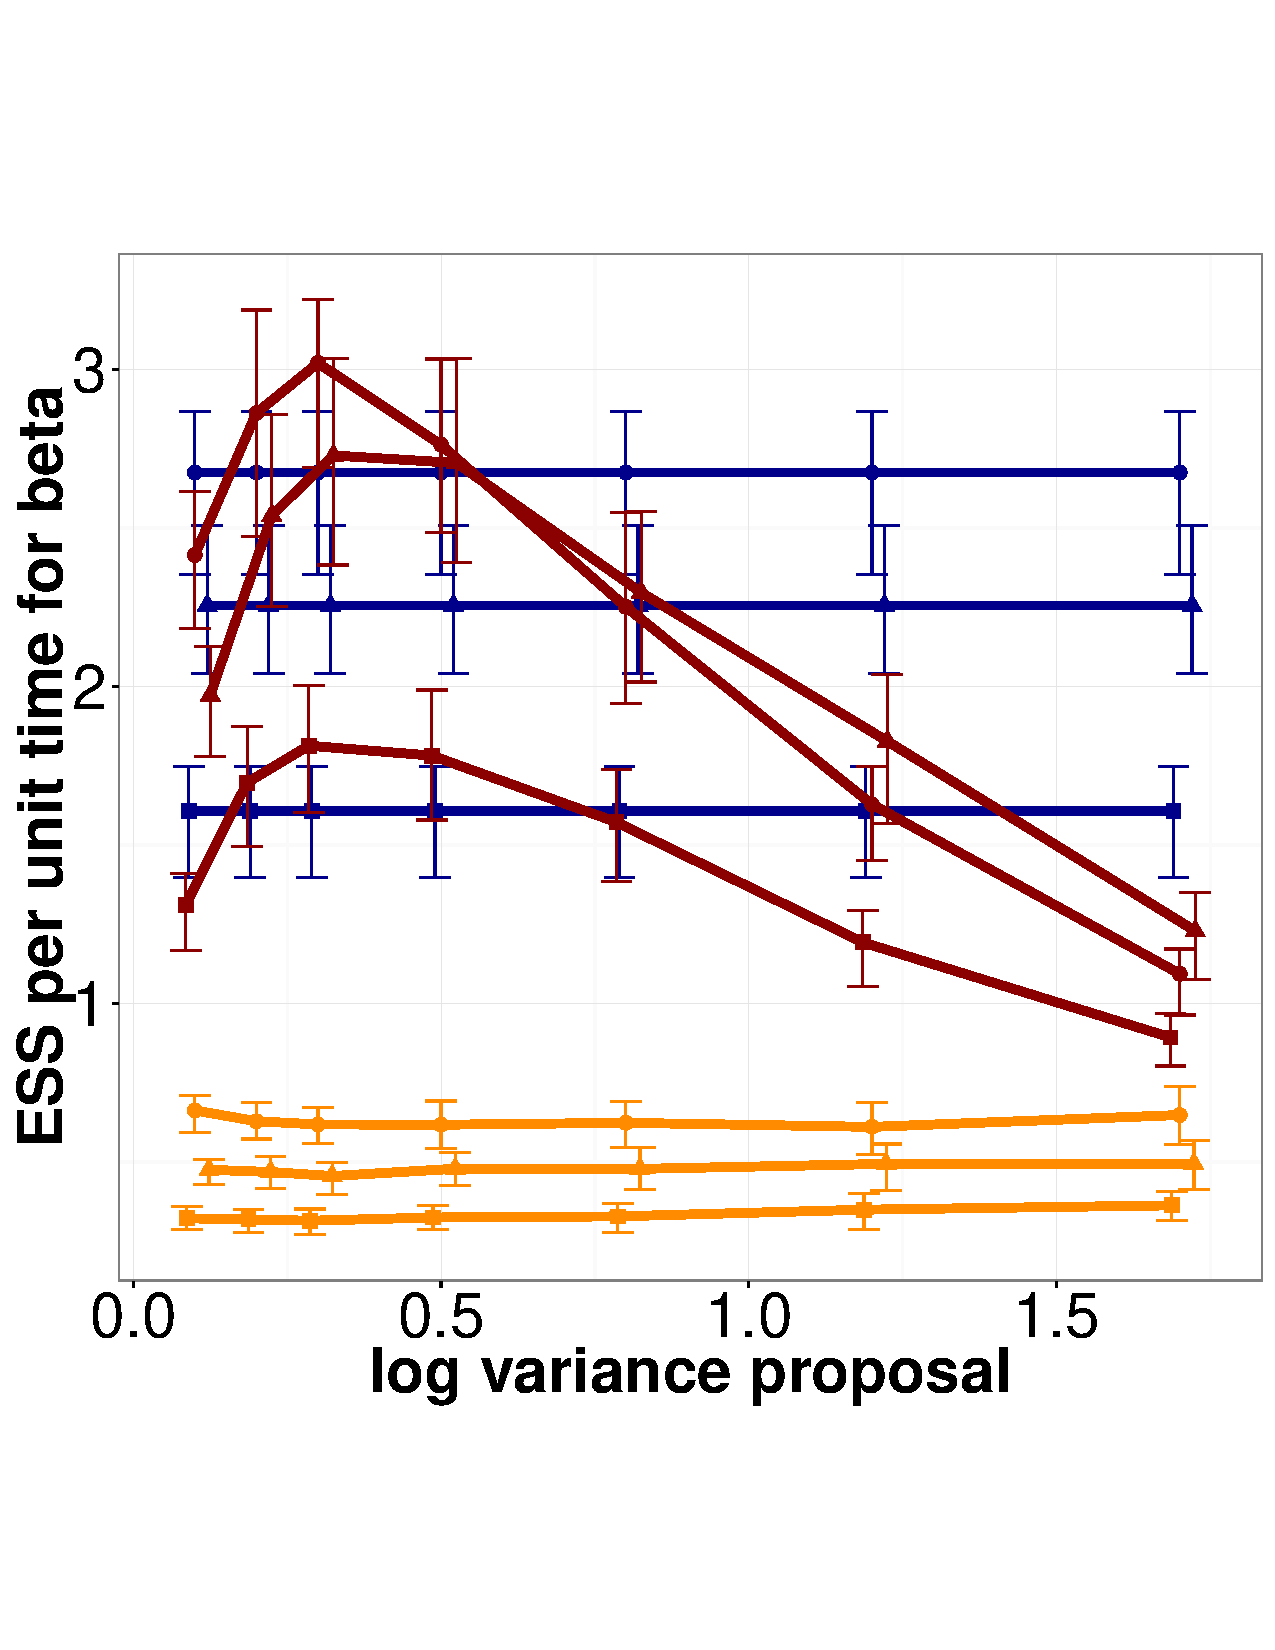
\includegraphics [width=0.70\textwidth, angle=0]{figs/q_5_beta.pdf}
    \vspace{-0 in}
     \label{fig:ESS_Q_5}
  \end{minipage}
    \caption{ESS/sec for Immigration model (dim 5)}
  \end{figure}

  \begin{figure}%[b]
  \centering
  \begin{minipage}[!hp]{0.45\linewidth}
  \centering
    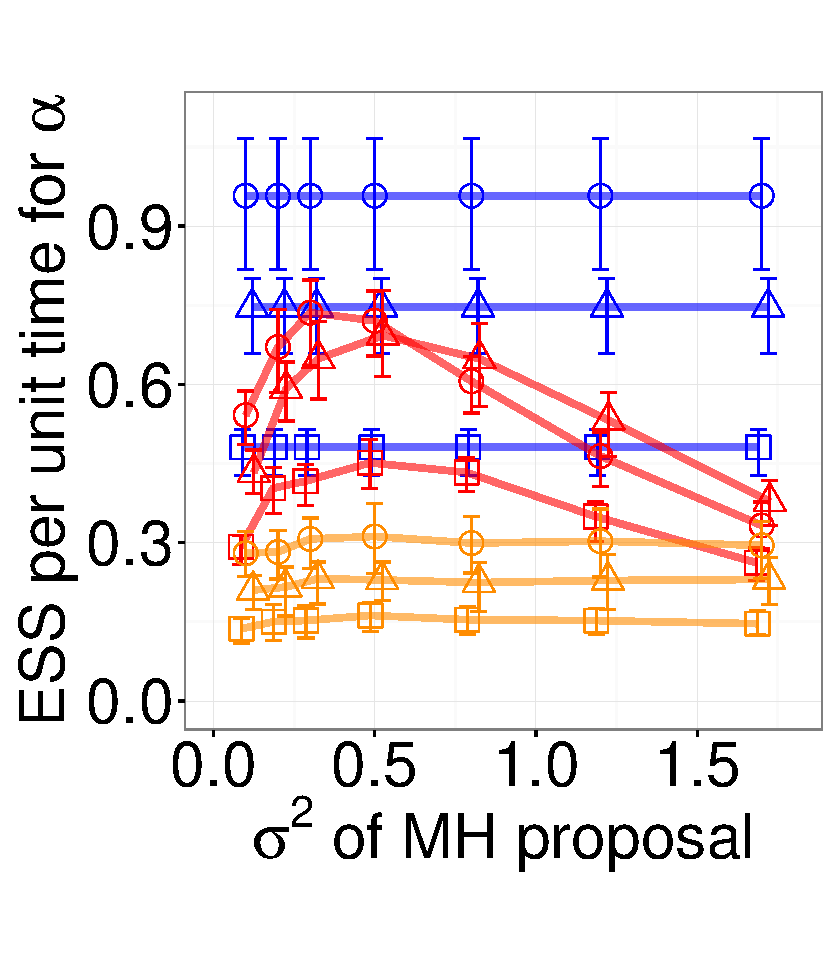
\includegraphics [width=0.70\textwidth, angle=0]{figs/q_10_alpha.pdf}
      \end{minipage}
  \begin{minipage}[!hp]{0.45\linewidth}
  \centering
    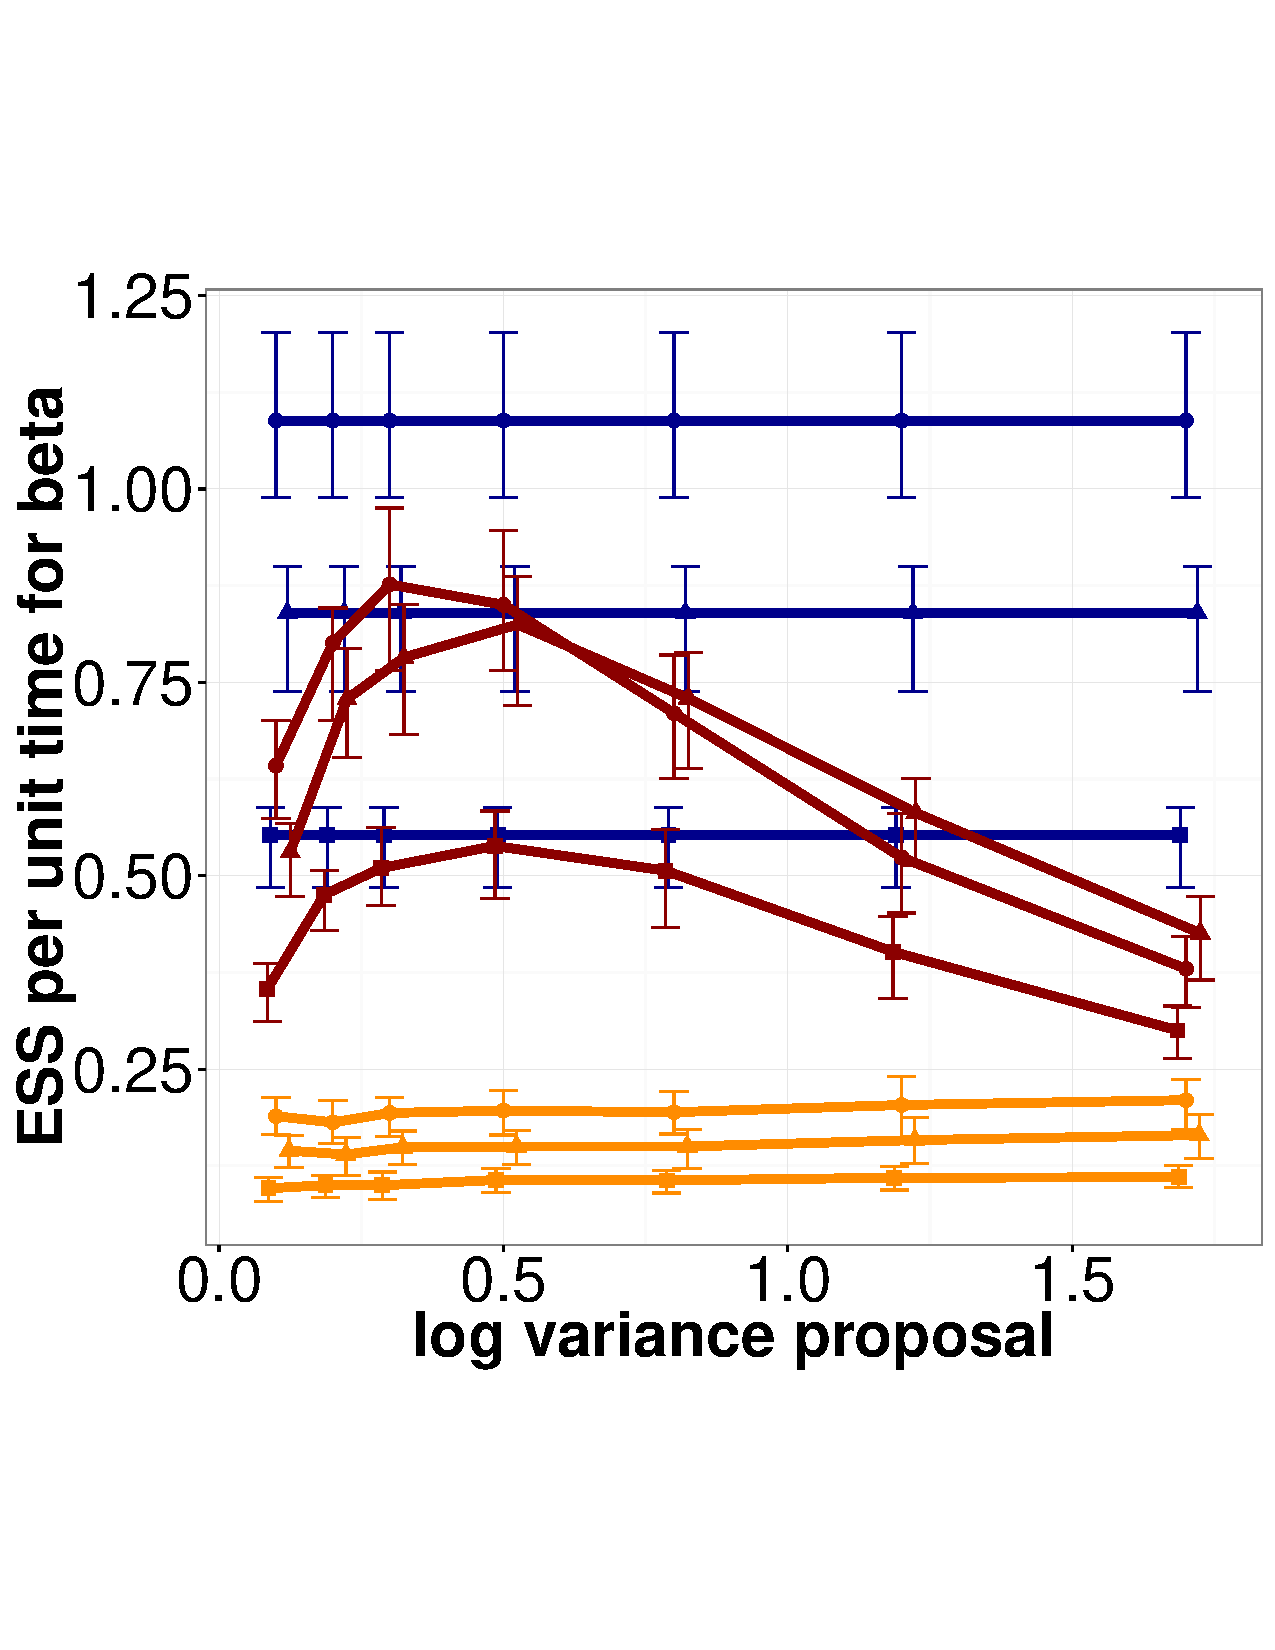
\includegraphics [width=0.70\textwidth, angle=0]{figs/q_10_beta.pdf}
    \vspace{-0 in}
     \label{fig:ESS_Q_10}
  \end{minipage}
    \caption{ESS/sec for Immigration model (dim 10)}
  \end{figure}

\begin{figure}
  \begin{minipage}[!hp]{0.45\linewidth}
  \centering
    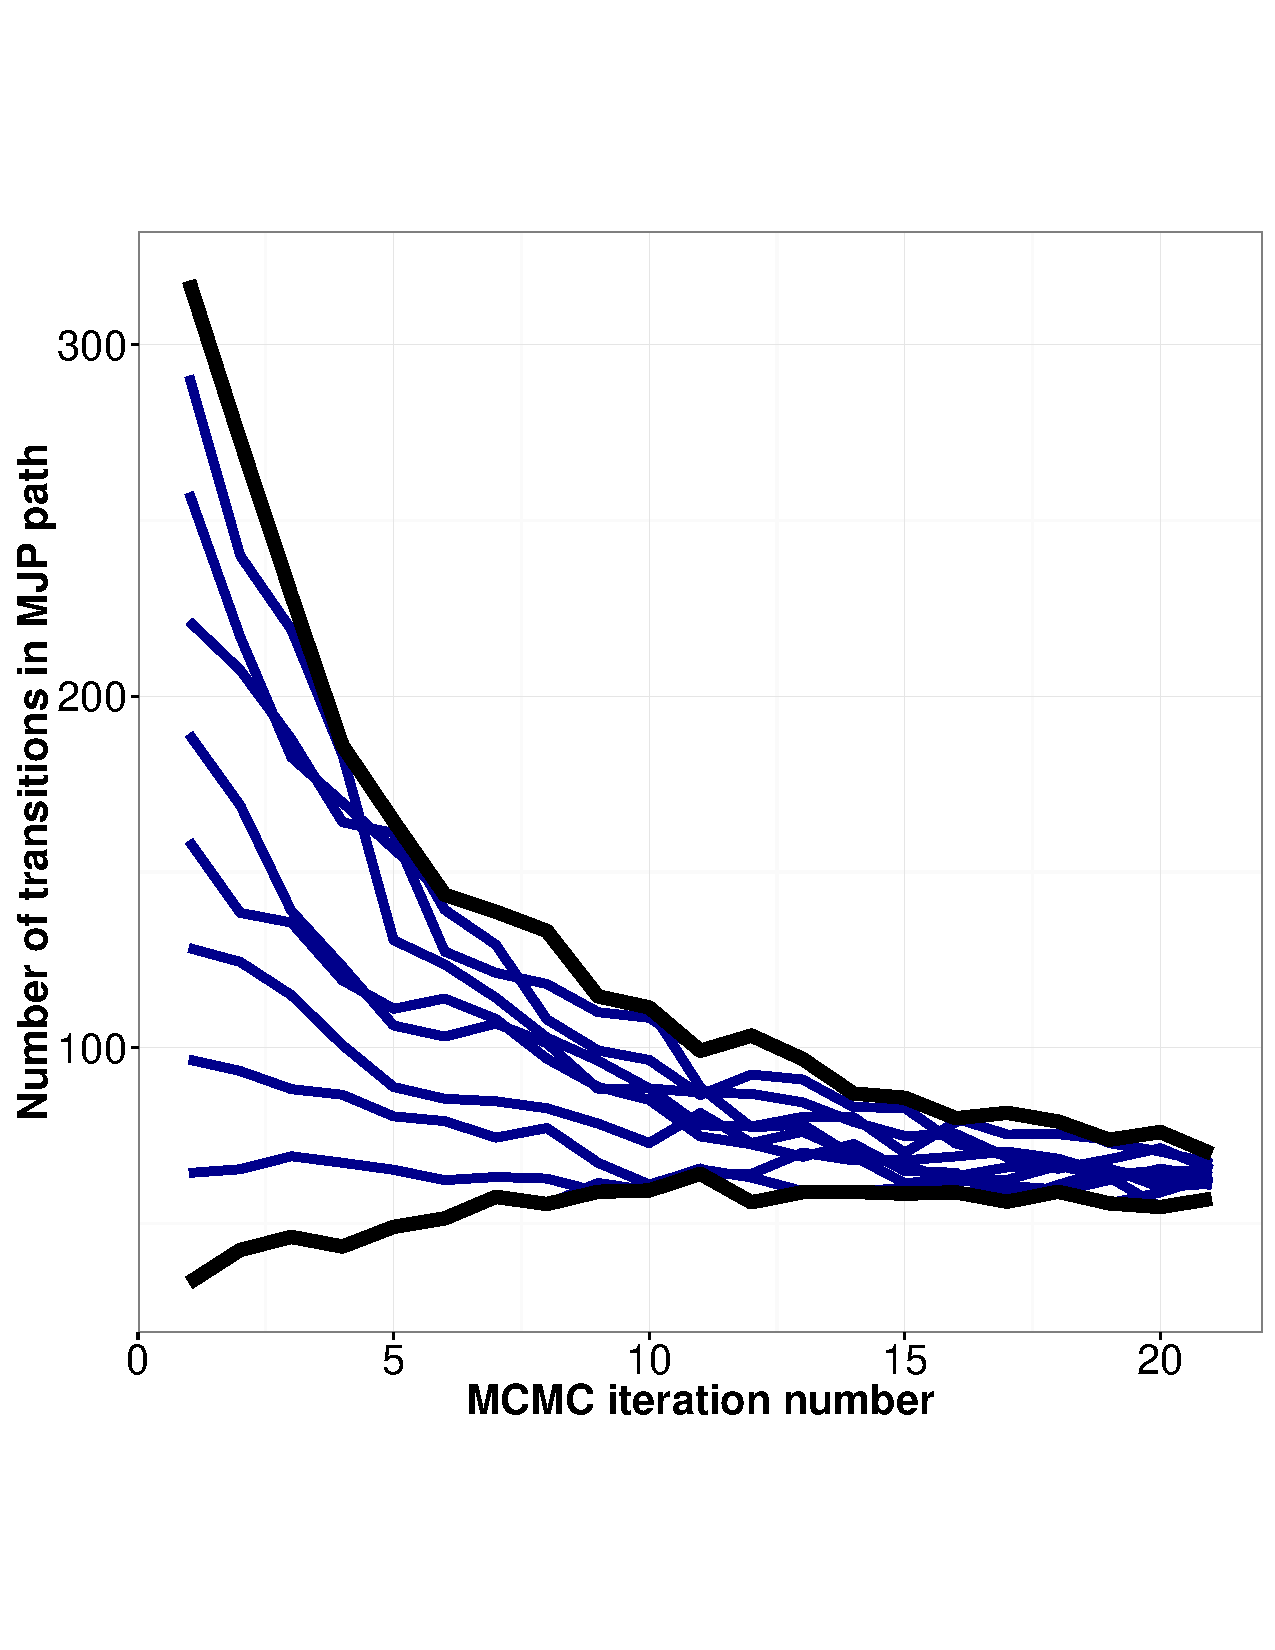
\includegraphics [width=0.70\textwidth, angle=0]{figs/q3_k2_path_transition.pdf}
    \vspace{-0 in}
    \caption{Trace plot of the number of MJP transitions for different initializatoins for immigration model.}
     \label{fig:ESS_EXP_TRANSITION}
  \end{minipage}

\end{figure}
\section{DNA evolution JC69 model }~
  \begin{figure}[H]
  \centering
  \begin{minipage}[!hp]{0.45\linewidth}
  \centering
    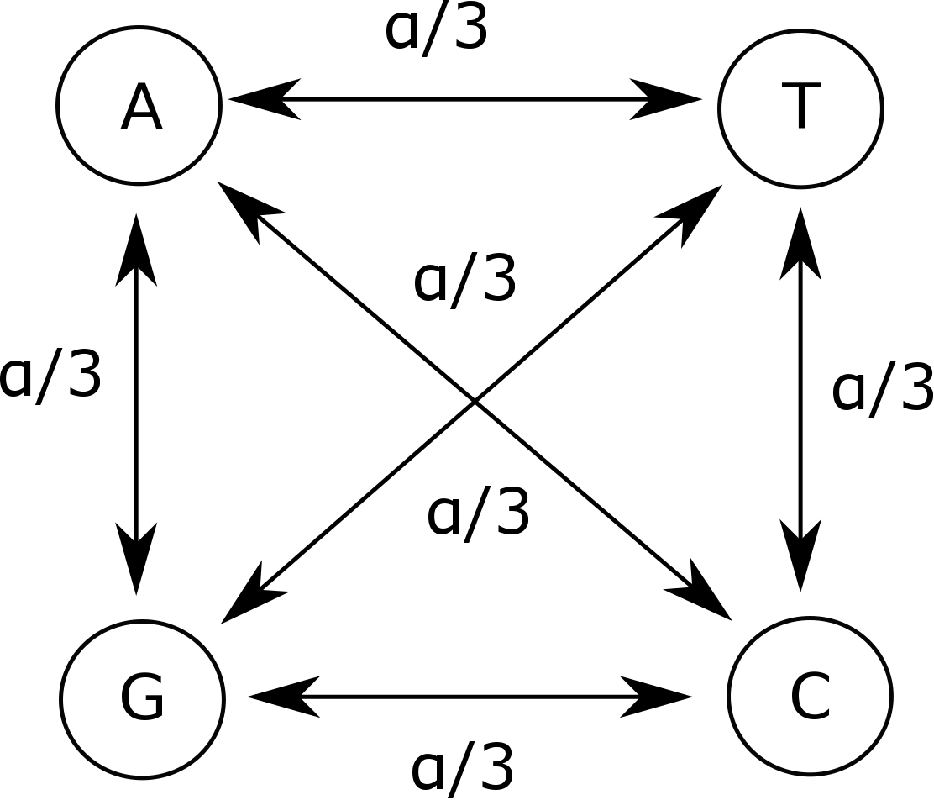
\includegraphics [width=0.70\textwidth, angle=0]{figs/jcplot.png}
      \end{minipage}
    \caption{exp model}
  \end{figure}

JC69 is the simplest substitution model. There are several assumptions. It assumes equal base frequencies and equal mutation rates. The only parameter of this model is $\alpha$. The overall substitution rate is therefore $3\alpha$. The state space is $\{1, 2, 3, 4\}$, representing $\{A, T, C, G\}$.\noindent Assume: $S = [S_0,S_1, ...,S_N] \;, T = [t_0(t_{start}), t_1,...,t_N, t_{N+1}(t_{end})]$, and y as observations.\\
$$A_i =: A_{i,i} = -3\alpha, \; \; i =0,1,...,N$$ $$A_{i, j} = \alpha, \; \; i \neq j.$$
If we assume the prior of $\alpha$ is $Gamma(\mu,\lambda)$\\
$$p(\alpha) = \frac{\lambda^\mu}{\Gamma(\mu)}\alpha^{\mu -1}e^{-\lambda \alpha} $$.
Then we can get the posterior distribution $$f(\alpha | s_0,S,T)$$ as follows.
$$ f(\alpha| s_0,S,T) \propto \exp(-(\lambda + 3(t_{end} - t_{start}))\alpha) \alpha^{\mu + N -1} .$$
$\alpha | s_0,S,T$ is following $Gamma(\mu+ N,\lambda + 3(t_{end} - t_{start}))$\\
\section{Experiments}
In the following, we evaluate a Python implementation of our algorithms compared to other exact samplers which include Gibbs sampler and Particle MCMC sampler. We consider three different dimensions which are 3, 5, and 10 and three different k which are 1.5, 2, and 3. We generated random parameters $\alpha$, $\beta$ from prior distributions ($Gamma(3,2), Gamma(5, 2)$), and used this to construct the transition matrix A. Then we generate an MJP trajectory with a uniform initial distribution over states. The state of this MJP trajectory was observed via a Normal distribution with mean equal to the value of state and variance 1, and posterior samples given the observations were produced by a Python implementation of our algorithm. 100 MCMC runs were performed, each run consisting of 10000(Varies among different dimensions) iterations. For each run, the number of transitions as well as the time spent was calculated, and effective sample sizes (ESSs) of these statistics (the number of independent samples with the same `information' as the correlated MCMC samples) were calculated using R-CODA (Plummer et al., 2006). The overall ESS of a run is defined to be the mean ESS across all these ESSs.

  \begin{figure}%[b]
  \begin{minipage}[!hp]{0.45\linewidth}
  \centering
    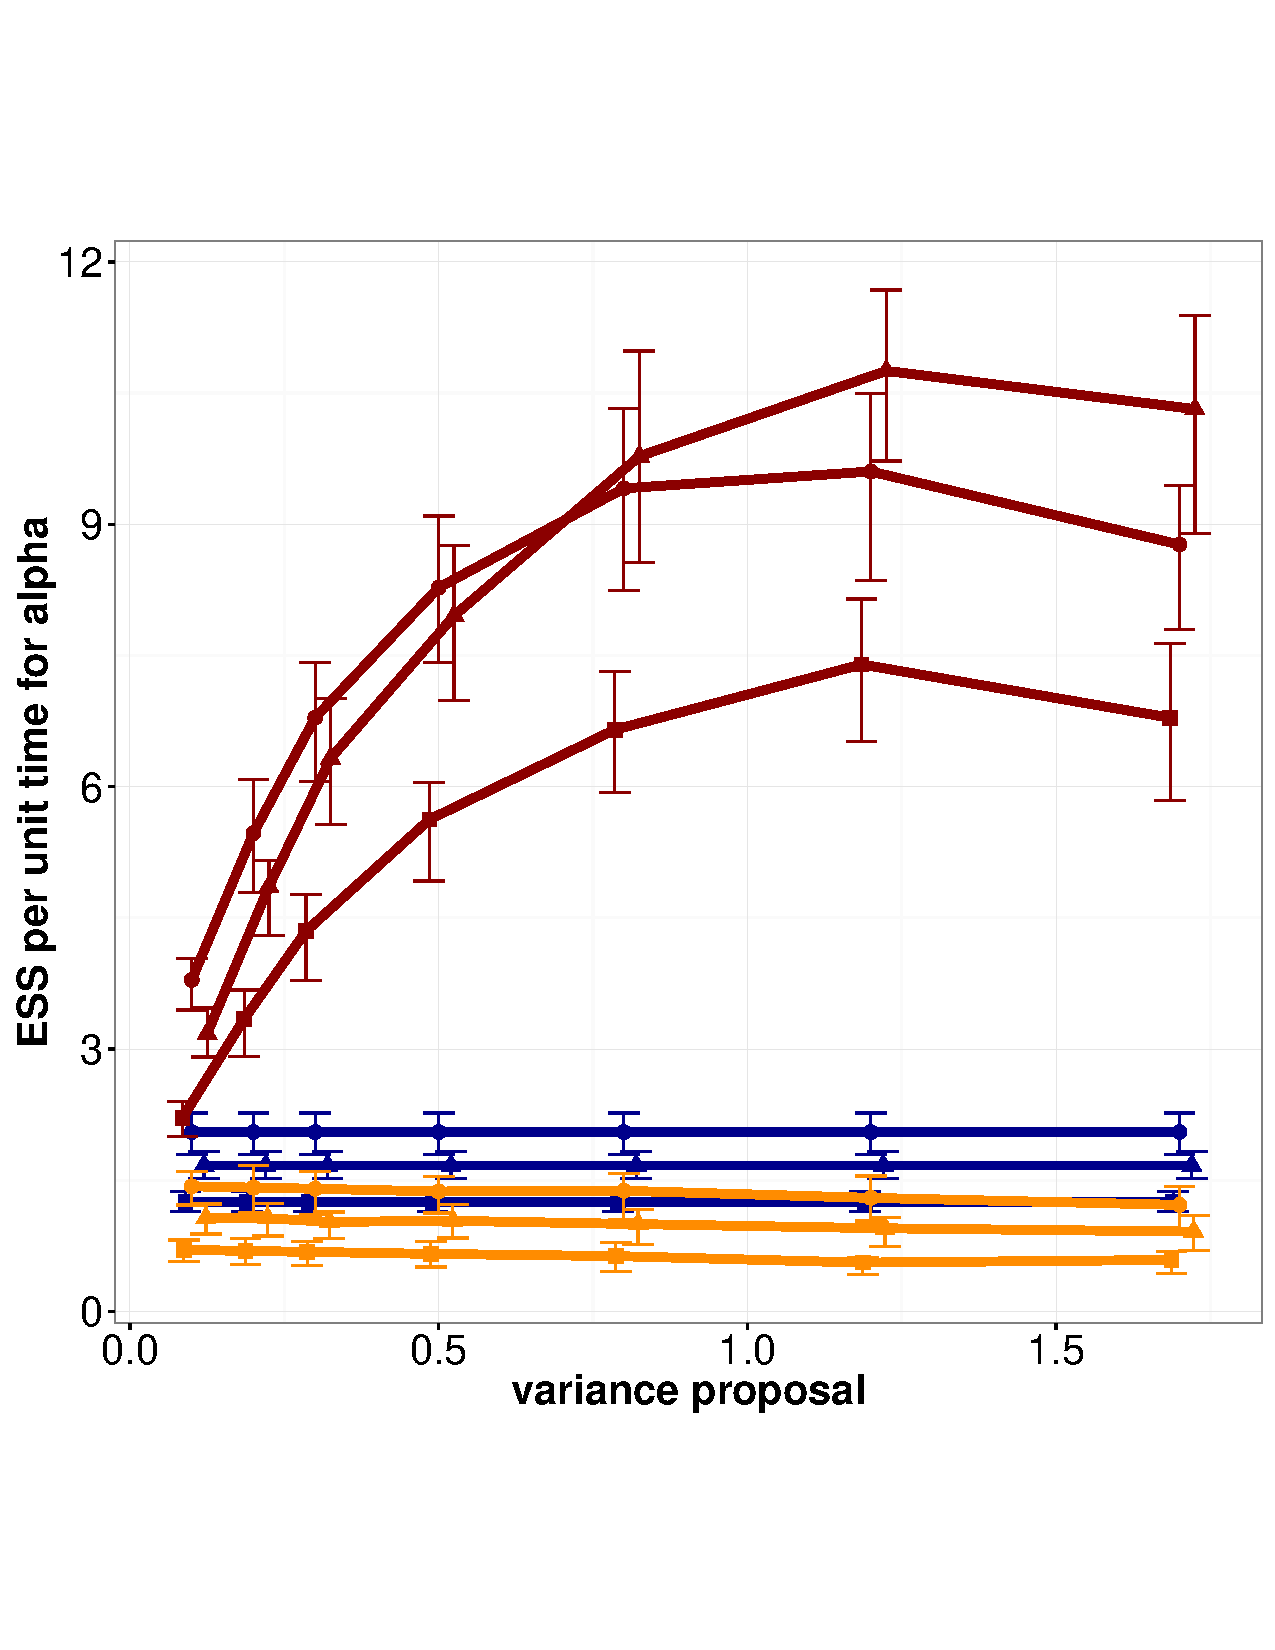
\includegraphics [width=0.70\textwidth, angle=0]{figs/jc.pdf}
    \vspace{-0 in}
    \caption{ESS/sec for JC69 Model }
     \label{fig:ESS_JC}
  \end{minipage}
  \end{figure}








\bigskip
%\begin{center}
%{\large\bf SUPPLEMENTAL MATERIALS}
%\end{center}

%\begin{description}

%\item[Title:] Brief description. (file type)

%\item[R-package for  MYNEW routine:] R-package �MYNEW� containing code to perform the diagnostic methods described in the article. The package also contains all datasets used as examples in the article. (GNU zipped tar file)

%\item[HIV data set:] Data set used in the illustration of MYNEW method in Section~ 3.2. (.txt file)

%\end{description}

~\cite{RaoTeh13}
~\cite{RaoTeh12}
~\cite{Andrieu10}
~\cite{Andrieu09}
~\cite{Golightly15}
~\cite{Andrieu102}
~\cite{Liu94}
~\cite{Neal12}
~\cite{Neal03}
\bibliography{bibfile}
\bibliographystyle{plain}
\end{document}
